% v3.0 released 22 May 2015

%%%%%%%%%%%%%%%%%%%%%%%%%%%%%%%%%%%%%%%%%%%%%%%%%%
\documentclass[fleqn,usenatbib,useAMS]{mnras}

\usepackage{graphicx}	% Including figure files
\usepackage{amsmath}	% Advanced maths commands
\usepackage{amssymb}	% Extra maths symbols
\usepackage{multicol}        % Multi-column entries in tables
\usepackage{bm}		% Bold maths symbols, including upright Greek
\usepackage{pdflscape}	% Landscape pages
\usepackage{enumitem}	% Including figure files
\usepackage{multirow}   % Allow multi-row cells in tables
\usepackage{xspace}
\usepackage{CJK}
\usepackage{longtable}
\usepackage{etoolbox}
\makeatletter
 \makeatother
%%%%%%%%%%%%%%%%%%%%%%%%%%%%%%%%%%%%%%%%%%%%%%%%%%
\newcommand{\teff}{$T_\mathrm{eff}$\xspace}
\newcommand{\logg}{$\log g$\xspace}
\newcommand{\feh}{$\mathrm{[Fe/H]}$\xspace}
\newcommand{\alphafe}{$\mathrm{[\upalpha/Fe]}$\xspace}
\newcommand{\vmic}{$v_\mathrm{mic}$\xspace}
\newcommand{\vbroad}{$v_\mathrm{broad}$\xspace}
\newcommand{\vrad}{$v_\mathrm{rad}$\xspace}
\newcommand{\Gaia}{\textit{Gaia}\xspace}
\newcommand\SB[1]{\textcolor{blue}{SB: #1}}
%%%%%%%%%%%%%%%%%%%%%%%%%%%%%%%%%%%%%%%%%%%%%%%%%%
\usepackage[T1]{fontenc}
\usepackage{ae,aecompl}
\usepackage{newtxtext,newtxmath}

%@arxiver{galah_rzxy_bstep.pdf, DR2_example_spectra.pdf, Abundance_overview_flag_0_snr_0.pdf}

\begin{document}
\begin{CJK*}{UTF8}{gbsn}
\label{firstpage}
\pagerange{\pageref{firstpage}--\pageref{lastpage}}

%%%%%%%%%%%%%%%%%%% TITLE PAGE %%%%%%%%%%%%%%%%%%%

\title{The GALAH Survey: Third Data Release}

% The list of authors, and the short list which is used in the headers.
% If you need two or more lines of authors, add an extra line using \newauthor
\author[Buder et al.]{Sven Buder$^{1,2,3}$\thanks{Contact e-mail: \href{mailto:buder@mpia.de}{buder@mpia.de}},
and~the~GALAH~collaboration \newauthor
(co-author order TBD in agreement with the SOFA)
\\
\\
(Affiliations listed after the references)}

% These dates will be filled out by the publisher
\date{Accepted 2020 Month Day. Received 2020 June 30}

% Enter the current year, for the copyright statements etc.
\pubyear{2020}

% Don't change these lines
\maketitle
\end{CJK*}

% Abstract of the paper
\begin{abstract}
This is the current draft of the accompanying paper for GALAH Data Release 3. \\
Please feel free to give feedback regarding both the analysis and the manuscript. \\
Our journey to discover the chemodynamic evolution of our Galaxy continues. With this third data release of the Galactic Archaeology with HERMES (GALAH) survey, we are publishing up to 30 abundances for XXXXX spectra taken of YYYYY stars with the HERMES spectrograph at AAT in Australia. This release includes observations of the main survey as well as the K2-HERMES, TESS-HERMES surveys, and additional projects of the bulge and open clusters. \\
Since the publication of GALAH DR2, we have been able to improve our spectrum analysis in several ways. We have updated our spectrum synthesis routines to take non-LTE departures into account for 11 elements, incorporate the astrometric information from the \Gaia satellite and photometric information from the 2MASS catalog and estimate element abundances line-by-line for as many elements as were feasible. Contrary to GALAH DR2, we are analysing all spectra only with the spectrum synthesis code Spectroscopy Made Easy (SME) to increase our accuracy throughout the parameter space. \\
Several Value-Added-Catalogs for stellar ages, stellar dynamics, and detailed abundance measurements accompany this data release. Together they provide a high-dimensional dataset to study the chemodynamic evolution of the local () Milky Way.
%
\end{abstract}

% Select between one and six entries from the list of approved keywords.
% Don't make up new ones.
\begin{keywords}
Surveys -- 
the Galaxy --
methods: observational --
methods: data analysis --
stars: fundamental parameters -- 
stars: abundances
\end{keywords}

%%%%%%%%%%%%%%%%%%%%%%%%%%%%%%%%%%%%%%%%%%%%%%%%%%

%%%%%%%%%%%%%%%%% BODY OF PAPER %%%%%%%%%%%%%%%%%%

%________________________________________________________________
\section{Introduction} \label{sec:introduction}

The field of Galactic Archaeology is in an transformation from single-star population studies towards large-scale structure analyses. Due to the limited information on the distances of stars, studies of the chemodynamic evolution of our Milky Way were previously limited to the nearby stars, but in the era of the \Gaia satellite, we can know use astrometric and photometric observables and their physical relations with spectroscopic quantities to improve the analyses of spectra and thus estimation of element abundances.

For the second data release of the GALAH survey \citep{Buder2018} we made use of data-driven approaches to improve both speed and precision of the spectrum analysis. These were performed almost entirely without non-spectroscopic information for individual spectra. The publication of \Gaia DR2 \citep{Brown2018, Lindegren2018} provided 5-parameter astrometry for 1.3 billion stars and can be understood as a game changer for stellar analysis.


%________________________________________________________________
\section{Target selection, observation, reduction} \label{sec:selection_observation_reduction}

\subsection{Target selection}

% This figure was created with the notebook GALAH_DR3/input/galah_dr3_input.ipynb
\begin{figure*}
\centering
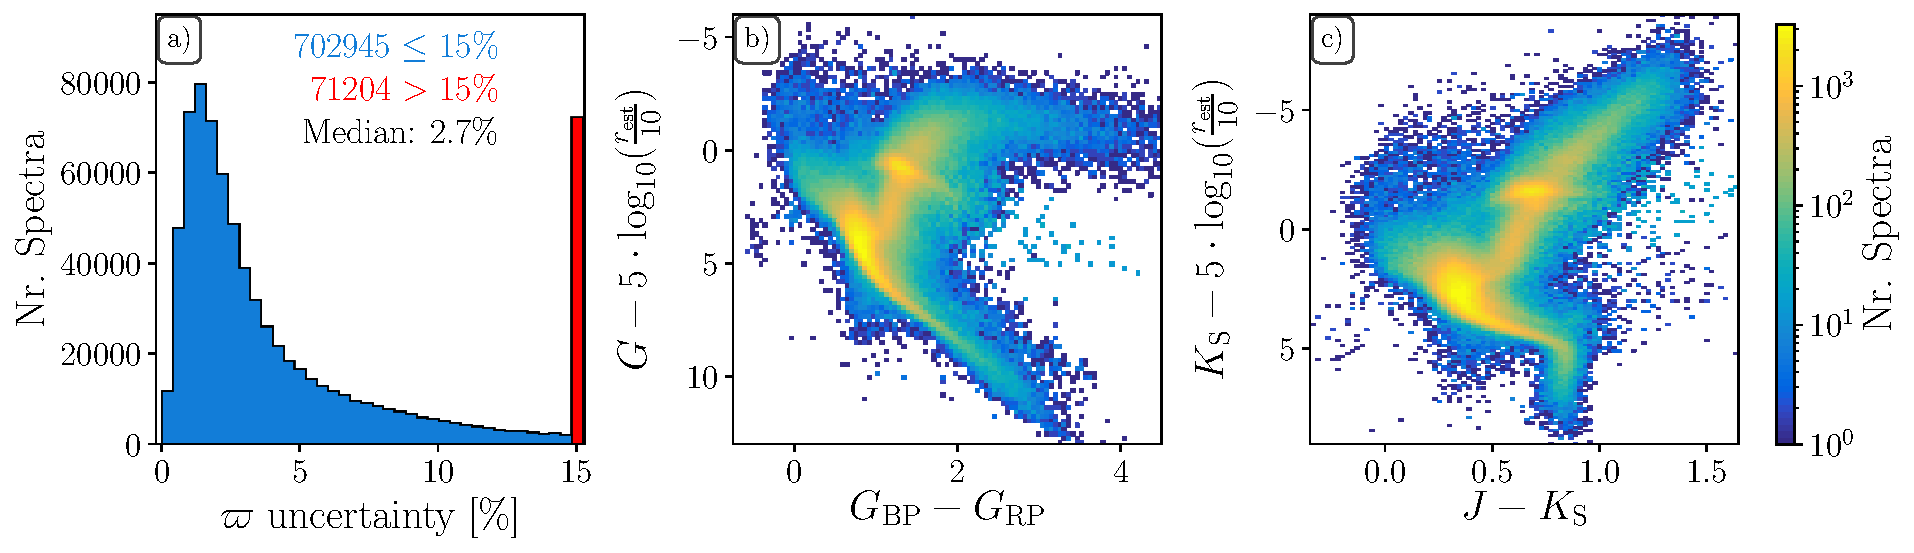
\includegraphics[width=\textwidth]{figures/plot_parallax_quality_and_cmds.pdf}
\caption{Overview of astro- and photometric information of the stars observed by GALAH until \SB{February 2019}. Panel a) shows the unprecedented parallax ($\varpi$) uncertainty provided by \Gaia DR2 with 702945 (91\%) spectra below 15\% (blue) and 71204 (9\%) spectra with uncertainties above 15\% (red, truncated). Panel b) shows a color-magnitude diagram as observed with the optical \Gaia passbands, whereas panel c) shows a color-magnitude diagram as observed with the infra-red 2MASS passbands. \SB{Note that not all of these stars are included in GALAH DR3}.}
\label{fig:plot_parallax_quality_and_cmds}
\end{figure*}

Parallaxes are now available for almost all stars observed by GALAH and a vast majority of them are very precise, see Fig~\ref{fig:plot_parallax_quality_and_cmds}. Overall, currently \SB{728651} spectra have matched parallax measurements, \SB{$85\,\%$ (619333)} even with parallax uncertainty $<10\,\%$. When dividing the sample into giants ($\textsc{teff} < 5500\,\mathrm{K}$ and $M_{K_S} < 2\,\mathrm{mag}$), \SB{$93\,\%$ (454406/488192)} of the observed dwarf spectra have parallax uncertainties below $10\,\%$ and \SB{$69\,\%$ (164927/240459)} of the observed giant spectra have parallax uncertainties below $10\,\%$. The use of inferred distance estimates by \citet{BailerJones2018} delivers even more reliable distance estimates.

Additionally, the progress in the analyses of observations of the K2 campaigns is providing more and more asteroseismic information. The overlap between GALAH targets and K2 targets from campaign C1-C8 and C10-C13 has increased the number of stars with measured asteroseismic $\nu_\mathrm{max}$ values to almost 15,000 and covers almost the entire giant branch, that is $1.5 < \log g < 3.5$, with its various evolutionary stages.

The selection was based on 2MASS \citep{Skrutskie2006} magnitudes and due to their brightness, almost all stars of the GALAH observations have well measured 5D information from \Gaia \citep{Brown2018, Lindegren2018}. An overview of the astro- and photometric information of the observed spectra can be found in Fig.~\ref{fig:plot_parallax_quality_and_cmds}

Mention Fig.~\ref{fig:distance}

\begin{figure}
  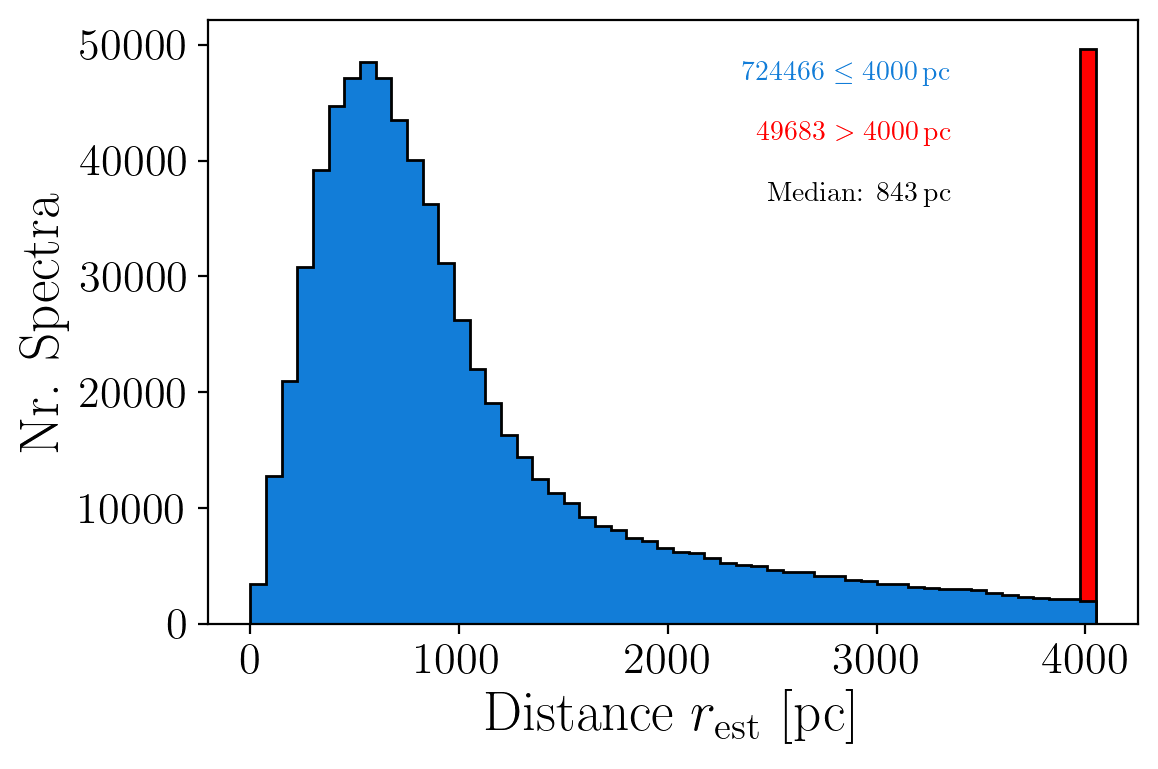
\includegraphics[width=\columnwidth]{figures/distance.png}
  \caption{Caption} 
  \label{fig:distance}
\end{figure}

Mention Fig.~\ref{fig:lb_overview_colored}

\begin{figure*}
\centering
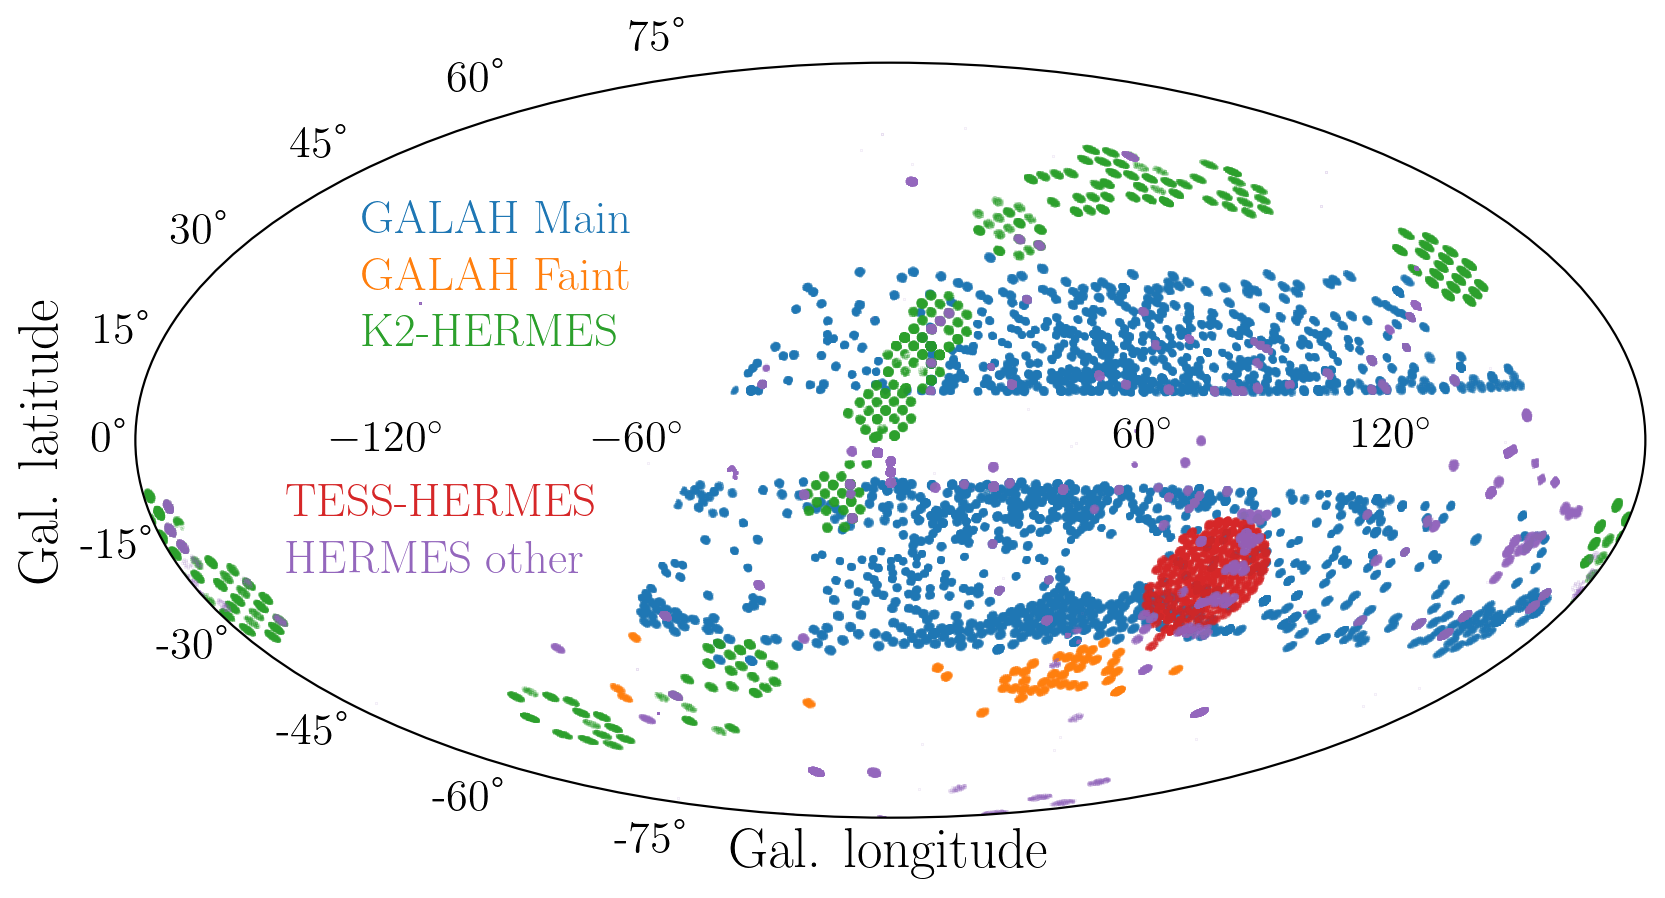
\includegraphics[width=\textwidth]{figures/lb_overview_colored.png}
\caption{Caption.}
\label{fig:lb_overview_colored}
\end{figure*}

\subsection{Observations}

Describe the observations from the beginning until the latest observations that will be included in 

\subsection{Reductions}

Short review of what was done.

Point out important changes since GALAH DR2 (was done with IRAF DR5.2 reduction).

%________________________________________________________________
\section{Data analysis} \label{sec:analysis}

%________________________________________________________________
\subsection{Analysis flow and changes with respect to DR2} \label{sec:analysis_flow}

\subsubsection{General workflow}

\begin{itemize}
\item SME only, no use of \textit{The Cannon} in this DR
\item Lay this out and motivate that by a figure, which shows 3 panels in the top for DR2 (Teff-logg, [Fe/H]-[alpha/Fe], [Fe/H]-A(Li)) and DR3 in the bottom
\item SME536, including changes as introduced by \citet{Piskunov2017}, but also with additional differences in the use of SME
\item using fundamental relation of surface gravity $\log g$ with available, non-spectroscopic information ($\varpi$ and $K_S$)
\item Workflow: 
\begin{enumerate}
	\item Estimate stellar parameters (\teff, \feh, \vbroad, \vrad from spectra, \logg via fundamental relation, \vmic via empirical relation)
	\item Validation of stellar parameters (see Sec.\ref{sec:validation_sp}), leading to an adjustment of the estimated atmospheric [Fe/H] (\textsc{sme.feh}) by adding $0.1\,\mathrm{dex}$\footnote{NB: This is not the final [Fe/H] as reported in this data release, but a pseudo iron abundance, estimated from H, Sc, Ti, and Fe lines.}
	\item Keep stellar parameters fixed and then estimate A(X) for element X. These can be done combined (write elements for which that was done) or on a line-by-line basis (write elements for which that was done).
\end{enumerate}
\end{itemize}

% This figure was created with the notebook GALAH_DR3/validation/comparisons/comparison_galah_dr2/galah_dr3_comparison_dr2.ipynb
\begin{figure*}
\centering
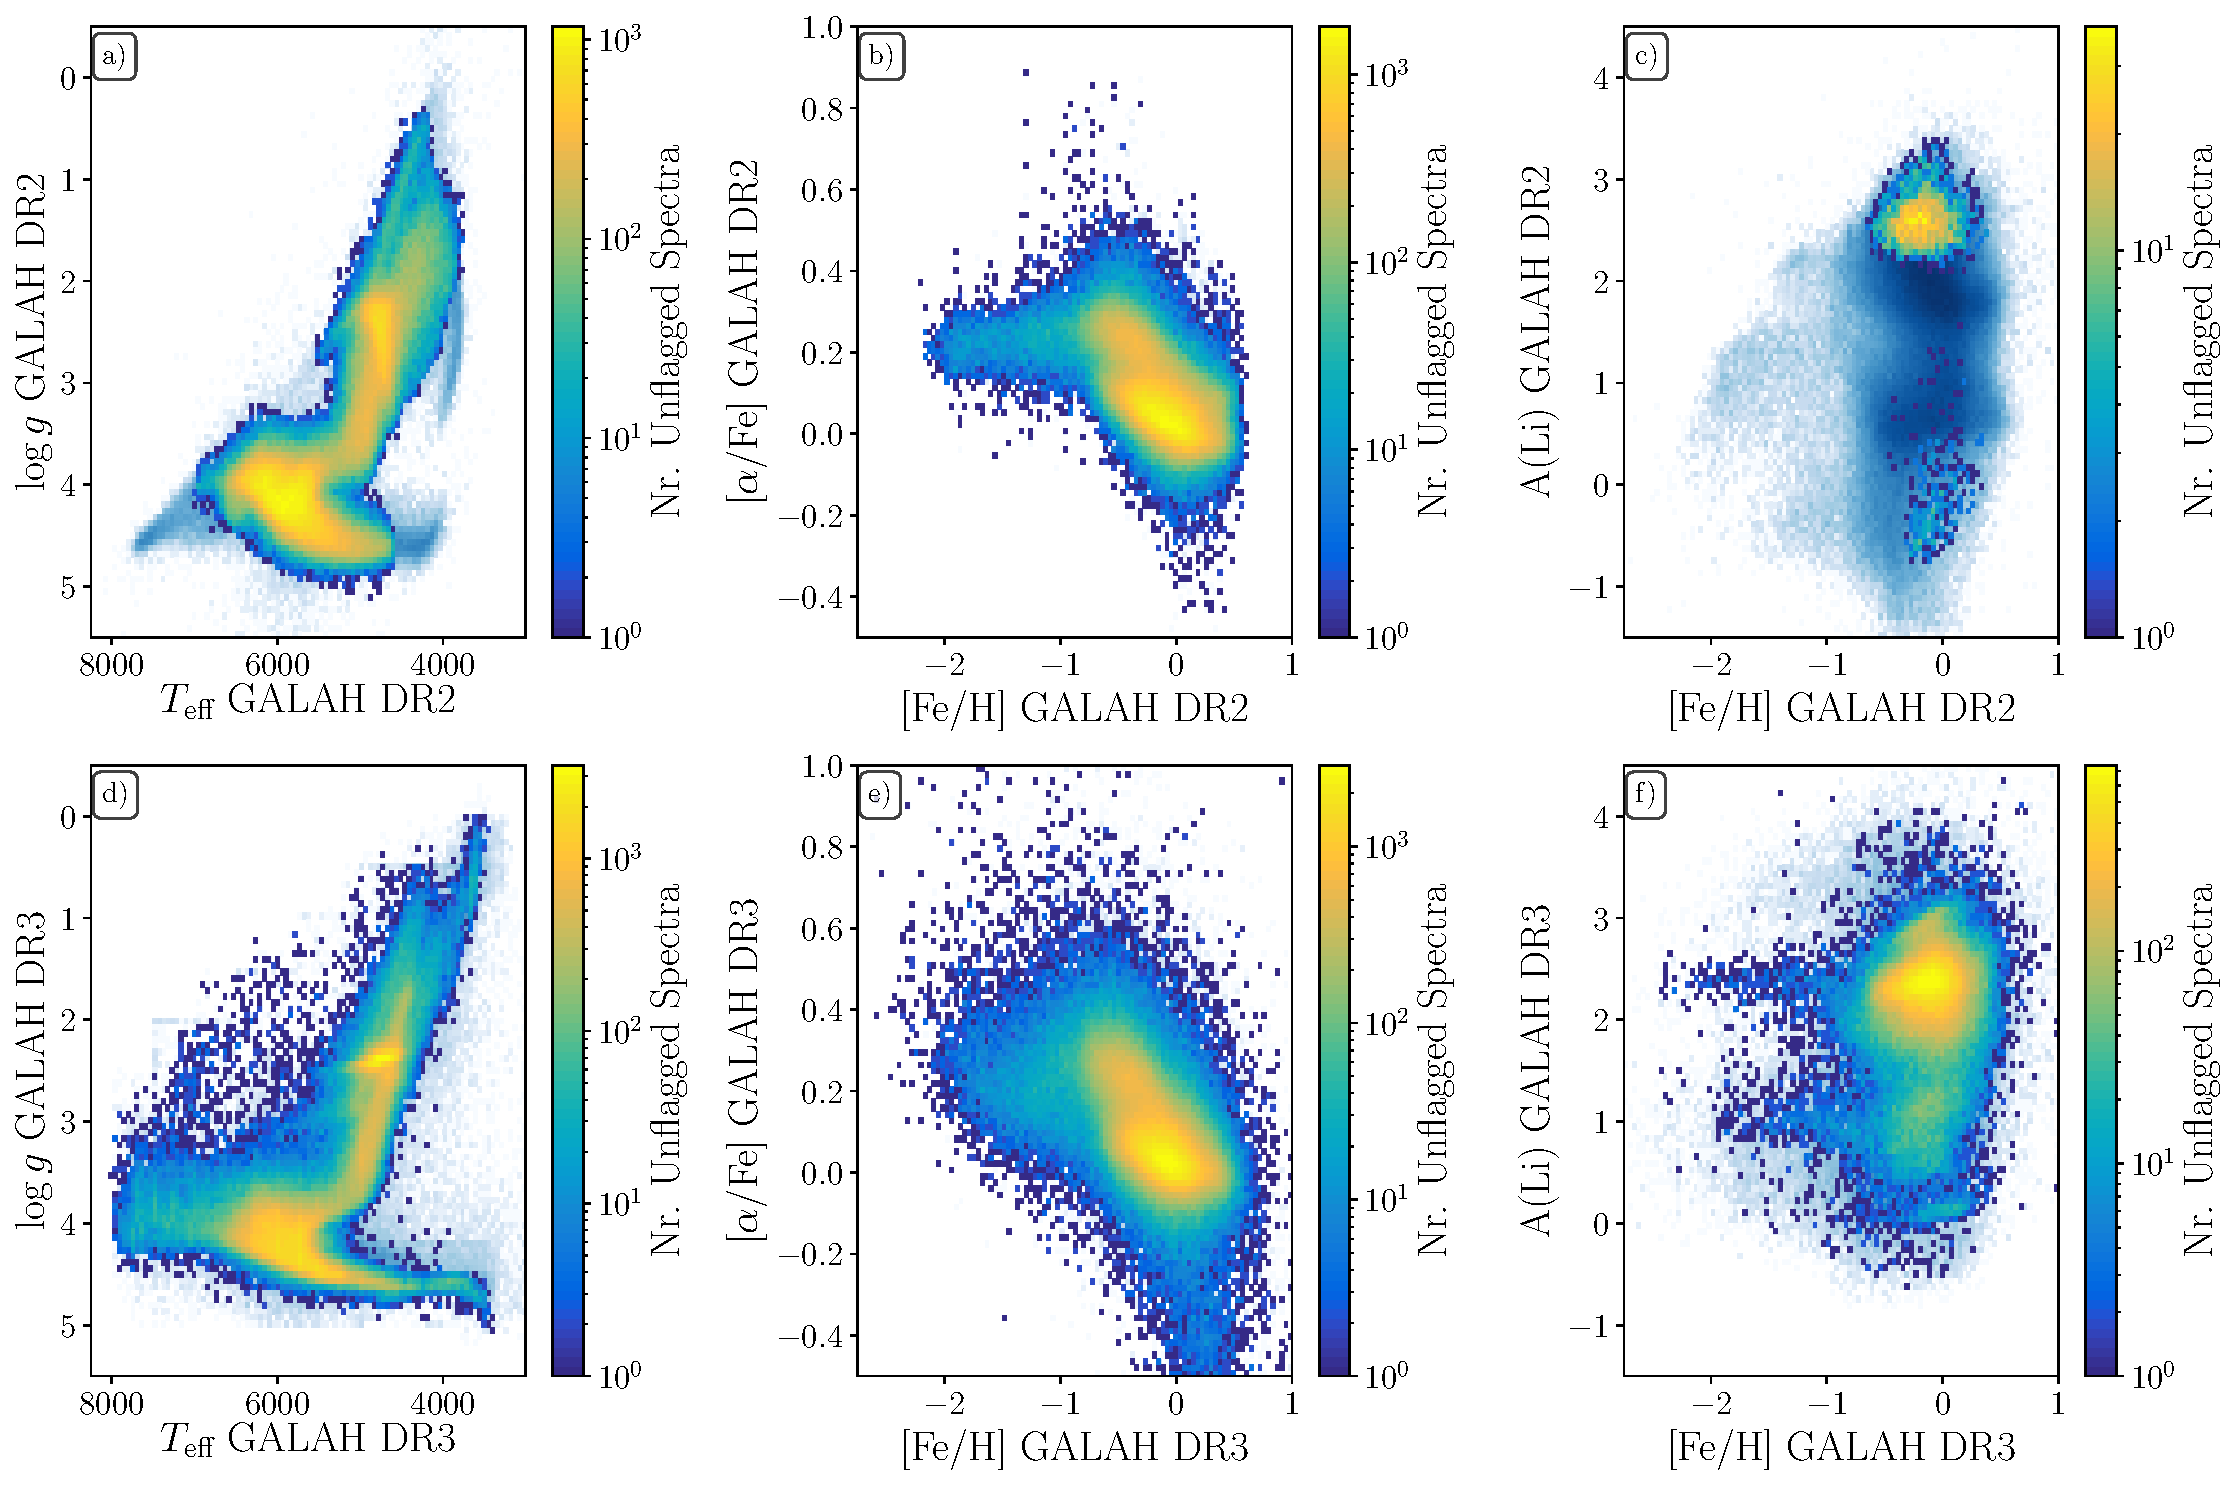
\includegraphics[width=\textwidth]{figures/galah_dr3_comparison_dr2.pdf}
\caption{Comparison of GALAH DR2 (upper panels) and GALAH DR3 (lower panels, this release). Pale blue contours indicate all measurements, whereas the colors as part of the colormaps indicate the unflagged measurements. Left panels show Kiel diagrams, i.e. \teff-\logg, for stars of DR2 (a) and DR3 (d). Middle panels show the abundance pattern of iron vs. $\upalpha$-process elements, i.e. \feh-\alphafe, for DR2 (b) and DR3 (e). Right panels show the absolute Li abundance as a function of iron abundance, i.e. \feh-A(Li), for DR2 (c) and DR3 (f). Note that the stars are not only the overlapping ones, but all measurements of the particular release.}
\label{fig:galah_dr3_comparison_dr2}
\end{figure*}

\subsubsection{Element abundance estimation}

Coincidentally with the significant improvements of stellar parameters, we have improved the determination of individual chemical abundances. Contrary to the previous GALAH analyses, we are now analysing element abundances as a simple error-weighted combination of all individual element line measurements. This approach has several advantages and we discuss several of them by looking at the combined and individual line abundances for Si in Fig.~\ref{fig:Si_abundance_zeropoint_differences}.

\begin{figure*}
\centering
\includegraphics[width=\textwidth]{figures/old/Si_compilation.pdf}
\caption[{Abundance trends for the Si I.}]{Abundance trends for the Si I. The top left panel shows the final combination of all Si I lines, whereas the other panels show the abundance trends for individual lines (indicated in the bottom left of each panel), when a global value $A(\mathrm{Si}) = 7.51$ is assumed for all lines. The black lines indicate the global solar value, whereas the black dotted lines indicate the individual solar value estimated from each line independently.}
\label{fig:Si_abundance_zeropoint_differences}
\end{figure*}

By using individual lines, we are less prone to unreliable line data, such as $\log gf$ values. Wrong oscillator strengths introduce a bias in the absolute abundance for each line. The Si lines at $5666\,\mathrm{\AA}$ is for example less accurate than the rest of the lines, because the oscillator strength that was measured in the laboratory \citep{GARZ,BL} is contaminated by a theoretically estimated lines by \citet{K07}. When such a line would be used for a global synthetic fit of [Si/Fe], they would introduce both a bias in the final abundance and parameter- as well as $S/N$-depending systematic trends. When the Solar abundance for these lines are however estimated independently from the others, they can still be used for the combined [Si/Fe] abundance, after applying individual Sun-based corrections to the absolute abundances.

The use of individual lines also allows to identify less reliable lines in terms of blending, reduction problems, and saturation. The Si lines at $6722$ and $7680\,\mathrm{\AA}$ are two line that display a significant amount of outliers towards higher and lower abundances than the other lines. In a global fit for [Si/Fe], they would hence introduce a higher scatter for the abundance.

We provide an simple error-weighted combination of the Mg, Si, Ca, and Ti lines as [$\upalpha$/Fe], see Fig.~\ref{fig:fe_h_alpha_fe}

\begin{figure*}
\centering
\includegraphics[width=\textwidth]{figures/old/fe_h_alpha_fe.pdf}
\caption[{[$\upalpha$/Fe] as a function of [Fe/H].}]{Error-weighted [$\upalpha$/Fe] estimated from individual measurements of Mg, Si, Ca, and Ti lines as a function of [Fe/H].}
\label{fig:fe_h_alpha_fe}
\end{figure*}

%________________________________________________________________
\subsection{Validation of stellar parameters} \label{sec:validation_sp}

To assess the quality of the stellar parameters, we resort to the commonly used comparison samples for accuracy, that is the GBS and the stars with asteroseismic information. For the precision assessment we use the internal uncertainty estimates and repeat observations of the same stars.  We calculate the final stellar parameter errors for a given parameter $X$ via 
\begin{equation}
e_\text{final}^2 (X) = e_\text{accuracy}^2(X) + e_\text{fit}^2(X) + e_\text{repeats}^2(X). \label{eq:final_error}
\end{equation}

We note that $e_\text{fit}^2(X)$ and $e_\text{repeats}^2(X)$ are typically expected to be the same tracer of precision and hence only their maximum value should be used, that is
\begin{equation}
e_\text{final}^2 (X) = e_\text{accuracy}^2(X) + \text{max} \left(e_\text{fit}^2(X) + e_\text{repeats}^2(X) \right).
\end{equation}

We elaborate on the choice of error combination when we assess the precision of the stellar parameters.

To identify those stars and spectra with less or unreliable information, we have implemented a combination of the flagging algorithms already applied to GALAH DR2 \citep[see][]{Buder2019} and new algorithms.

\subsubsection{Accuracy of stellar parameters}

\paragraph*{\Gaia FGK benchmark stars (GBS)}

When comparing the estimated stellar parameters (blue error bars) for the observed GBS with those from \citet{Jofre2018a}, we do not find any significant biases regarding $T_\text{eff}$ and $\log g$, but had to correct a bias of $\mathrm{[Fe/H]}  = -0.10$ (underestimated [Fe/H]), see Fig.~\ref{fig:gbs_performance}. Underestimated temperatures for the hottest stars are still likely, but more testing is needed as the continuum normalisation has been improved and hydrogen has been implemented in non-LTE now. More importantly, the scatter with respect to the GBS values by \citet{Jofre2018a} has decreased significantly for $\log g$ and noticeably for $T_\text{eff}$ and $\mathrm{[Fe/H]}$ as can be seen in the diagram, where also results from a purely spectroscopic analysis are shown in black for the same stars.

\begin{figure*}
\centering
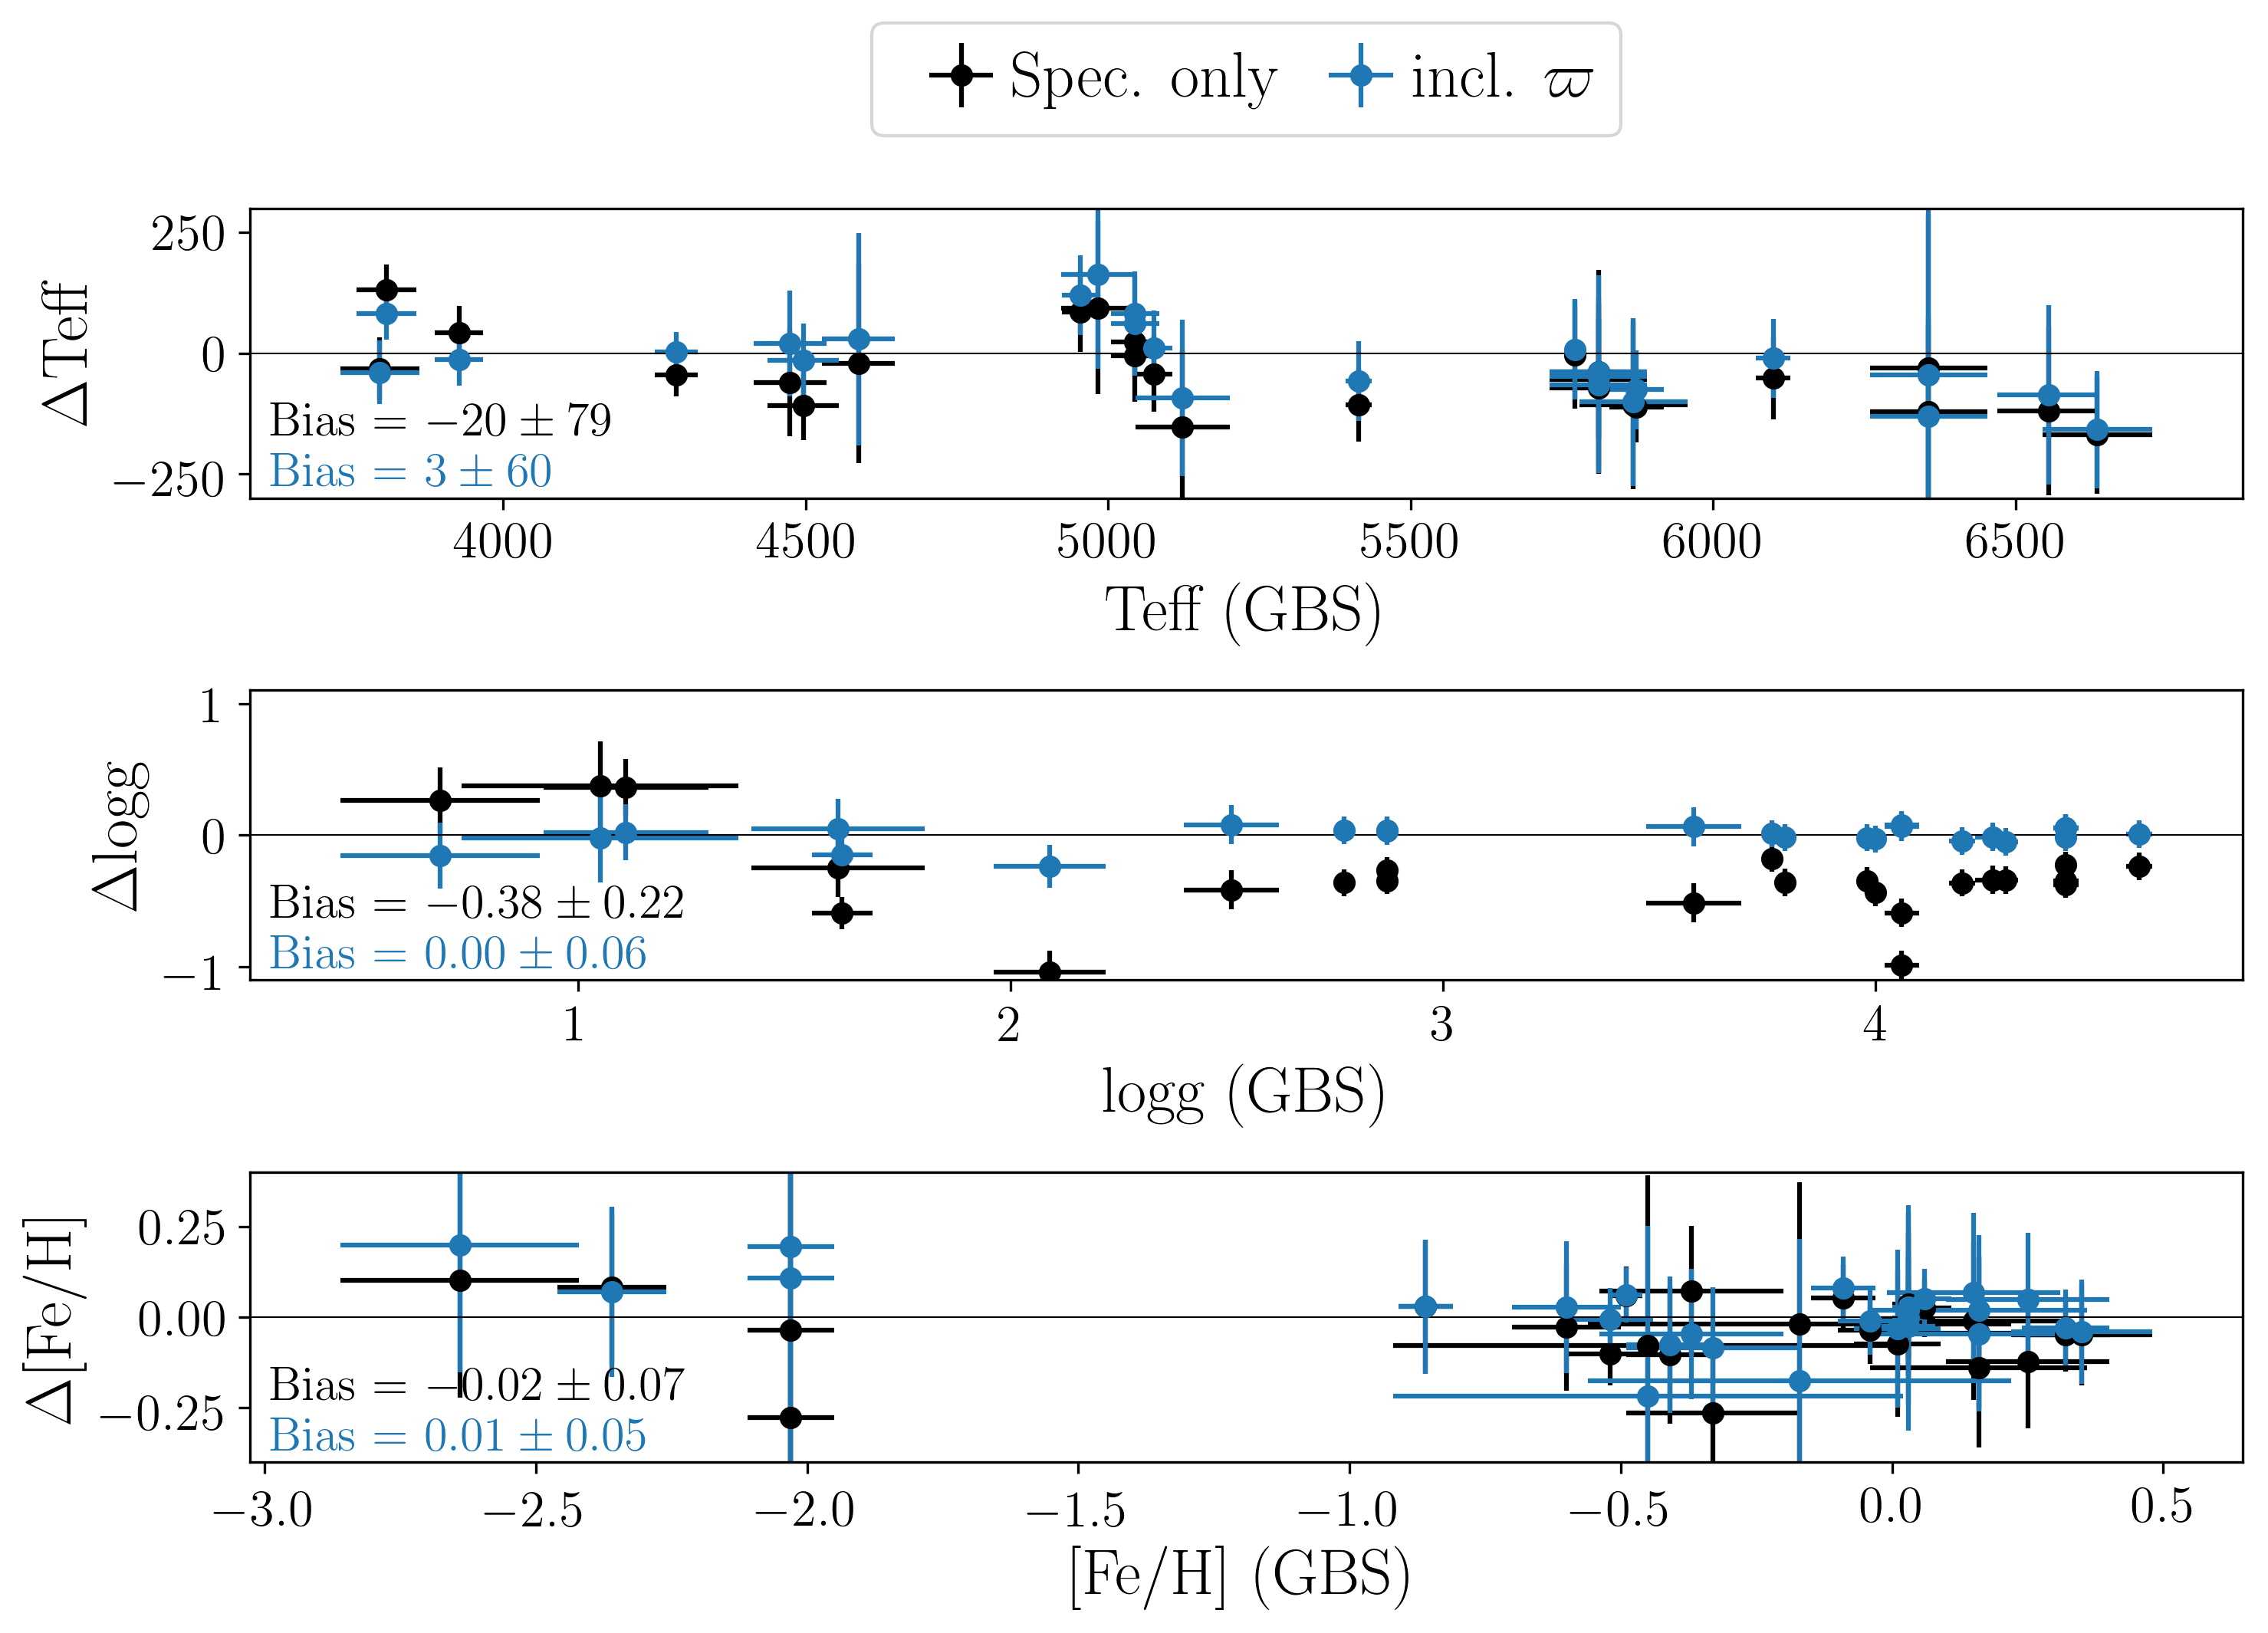
\includegraphics[width=0.8\textwidth]{figures/old/gbs_performance_free_lbol.png}
\caption[{Performance of GALAH synthesis pipeline with the `free' (black) and `bolometric' (blue) pipeline.}]{Performance of GALAH synthesis pipeline with the `free' (black) and `bolometric' (blue) pipeline. Difference as stated as GALAH - GBS.}
\label{fig:gbs_performance}
\end{figure*}

In addition, we have been able to show that the pipeline can now also estimate stellar parameters of core-helium burning stars, including horizontal branch stars. Horizontal branch stars have not been included in the training set used for the analysis of GALAH DR2. We have noted however, that for very distant stars (e.g. the bright stars in the LMC), the inferred distances by \citet{BailerJones2018} are too low and lead to an overestimated $\log g$.

\paragraph*{IRFM temperatures}

\paragraph*{Stars with asteroseismic information}

The biases between the `asteroseismic' and `bolometric' pipeline for the stellar parameters are minor as discussed in Sec.~\ref{sec:analysis_gaia}. However, we find systematic differences between photometric (isochrone) and asteroseismic masses of RC stars, in particular for the most metal-rich isochrones. The isochrone grid is very dense in this regime and and spectroscopic parameters of the RC stars overlap strongly with those of RGB stars. \citet{An2019}, however, found similar differences and suggest that standard RC isochrone models need to be re-examined. Additionally, we suggest that the validity of the asteroseismic scaling relations \citep[see e.g.][]{Epstein2014, Huber2017, Viani2017, Pinsonneault2018} for the most metal-poor and metal-rich stars should be examined further. 

\begin{figure*}
\centering
\includegraphics[width=\textwidth]{figures/old/logg_seis_validation_largesample.pdf}
\caption[{All stars with asteroseismic information from the K2 asteroseismic analyses (Sharma and Stello, priv. communication).}]{All stars with asteroseismic information from the K2 asteroseismic analyses (Sharma and Stello, priv. communication). The colorbar indicates spectra with good asteroseismic information. Misclassifications, that is clear dwarfs with underestimated $\nu_\text{max}$ values are shown in orange, an overdensity with wrong $\nu_\text{max}$ values at $\log g = 3$ is shown in blue and significant outliers are shown in green.}
\label{fig:all_seismic}
\end{figure*}

In addition to the sample of 3175 spectra that we analysed with different pipelines, we have examined the accuracy of our surface gravities for an even larger sample of stars with asteroseismic information from the complete K2 analysis (Sharma and Stello, priv. communication). We compare the $\log g$ estimated from $T_\text{eff}$ and $\nu_\text{max}$ with the $\log g$ from the `bolometric' pipeline in the left panel of Fig.~\ref{fig:all_seismic}. As stated in Sec.~\ref{sec:analysis_gaia}, the K2 data is expected to currently only allow reliable asteroseismic results for giants with $1.5 < \log g < 3.0$. The comparison of the `asteroseismic' and `bolometric' pipeline showed that the K2 pipelines also estimate wrong $\nu_\text{max}$ value for 7.5\% of the sample (orange misclassifications), that is $\nu_\text{max}$ values that are too low for the actual $\log $. We identify such wrong classifications in Fig.~\ref{fig:all_seismic} in orange and blue. The latter color indicates an overdensity of wrong $\nu_\text{max}$ values suggesting $\log g = 3.0$, although the actual $\log g \sim 3.5$ is beyond the expected detection limit. Orange colors indicate all other misclassified stars, that is mainly dwarfs with significantly underestimated $\nu_\text{max}$ values. After cleaning the sample from these outliers, we estimate the systematic difference between the $\log g$ from the `bolometric' pipeline and $\log g$ from $T_\text{eff}$ and $\nu_\text{max}$ (see color coded distribution in Fig.~\ref{fig:all_seismic}) and find the same small bias as for the 3175 spectra, that is $-0.03 \pm 0.12$. The lower standard error of this measurements is $0.001$ indicates that this bias is even more significant.

\subsubsection{Precision of stellar parameters}

To estimate the precision of stellar parameters, we use both internal SME covariance errors and repeated observations of the same star. We have estimated the standard deviations of repeated observations for the same fiber, different fibers, and irrespective of the fibre and plot their standard deviations as a function of $S/N$ in CCD2 together with the median SME covariance errors in Fig.~\ref{fig:precision_sp} for the fitted stellar parameters $T_\text{eff}$, $\log g$, iron line abundance [Fe/H], the atmosphere iron abundance [Fe/H], rotational broadening $v_\text{broad}$, and radial velocity $r_\text{rad}$. 

\begin{figure*}
\centering
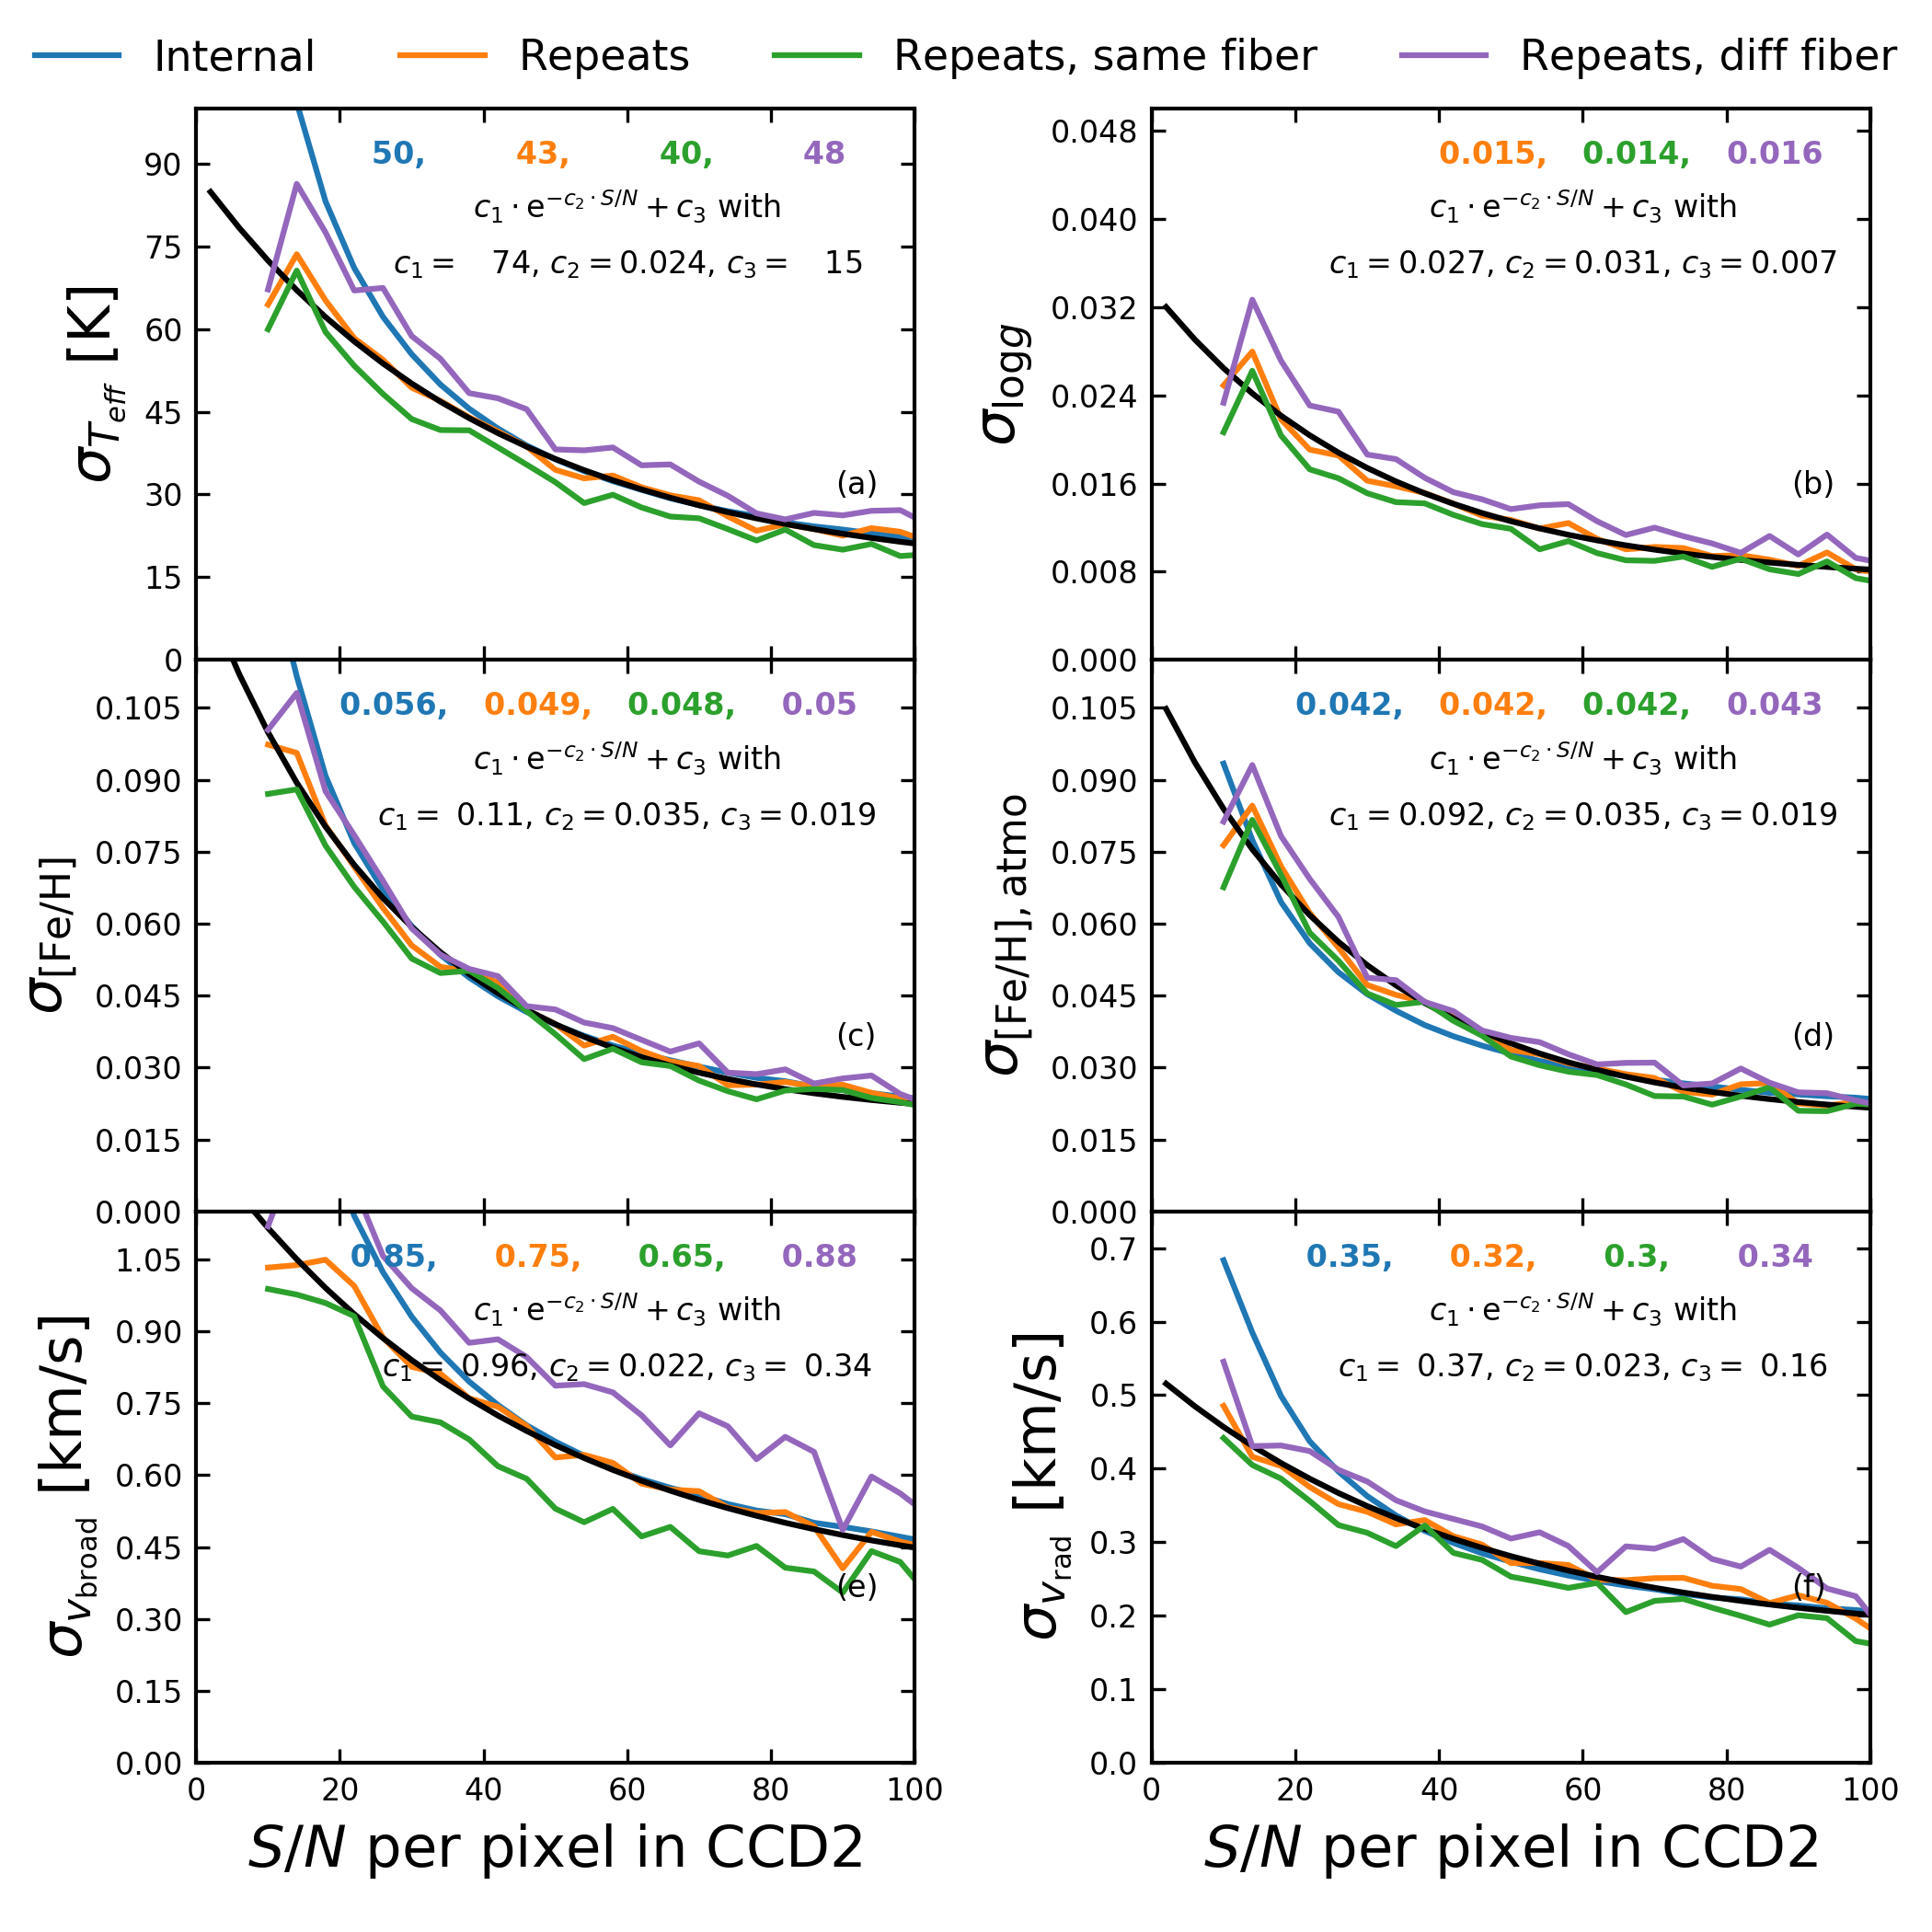
\includegraphics[width=0.9\textwidth]{figures/old/repeat_uncertainties_snr_flag0.pdf}
\caption[{Precision estimates for stellar parameters.}]{Precision estimates from internal SME covariance uncertainties (blue) as well as standard deviations from all (orange), same fibre (green), and different fibre (violet) repeat observations. The numbers in each panel indicate the uncertainties estimated for $S/N = 40$ per pixel, similar Fig. 15 from \citet{Buder2019}.}
\label{fig:precision_sp}
\end{figure*}

The trends of internal and repeat precision are expected to be similar, but we find that the uncertainties from the internal SME covariance uncertainties are typically significantly lower than those from repeat observations (with exception of $\log g$, which we discuss subsequently). As discussed when introducing the final error estimation with Eq.~\ref{eq:final_error}, the two precision estimates should be the same and a rescaling of the internal SME-based uncertainties would lead to a consistent precision measure. First estimates suggest that a rescaling with a factor of 2.5 yields an agreement of repeat observations and internal uncertainties for $T_\text{eff}$. For the other parameters, however, also an the uncertainty floors of the two precision estimates are different and we thus need to still explore more complex scaling relations. For the purposes of the internal data release, we hence decide to calculate the precision as a combination of both estimates. This allows to combine the individual estimate of the fit quality (through the internal SME-based uncertainty) with the general precision expected for a given $S/N$, which would otherwise be underestimated when only using to the internal uncertainty. In order to allow the estimation of the repeat precision $e_\text{repeats}$ for each spectrum, we fit an exponentially decreasing function to the orange repeat uncertainty distribution (shown as black line in Fig.~\ref{fig:precision_sp}).

We stress that $\log g$ values are not optimised from the $\chi^2$-determination of the spectra like the other parameters, but from Eq.~\ref{eq:bolometric_logg}. We thus sample the parameters used for Eq.~\ref{eq:bolometric_logg} via MC sampling to estimate the `internal' uncertainties for $\log g$. We note that in the current MC sampling, the parameters are sampled from fixed Gaussian distributions with $\sigma (M) = 0.1\cdot M$ as well as $\sigma (BC) = 0.1\,\mathrm{mag}$. $\sigma (T_\text{eff})$, $\sigma (D_\varpi)$, $\sigma (K_s)$, and $\sigma (A_{K_s})$ are sampled from their uncertainties. The internal standard deviation for $\log g$ is hence almost $S/N$ independent.

The comparison of the GALAH DR3 precision estimates with those from GALAH DR2 \citep{Buder2018} shows that the precision (for the median $S/N \sim 40$ of all spectra) has marginally improved, for example from $34\,\mathrm{K}$ for $T_\text{eff}$ of same fiber repeats to $27\,\mathrm{K}$. We note that for $\log g$ the repeat observation precision is significantly better by construction, that is it decreased from 0.060 for GALAH DR2 to 0.012 for GALAH DR3.

\section{Validation of element abundances} \label{sec:validation_ab}

\subsubsection{Accuracy of element abundances}

\paragraph*{Abundance zeropoints}

For several lines of the GALAH wavelength range, we are facing a different issue, that is that we can not use a Solar or sky flat spectrum for the accuracy assessment of the abundance, because the line is too weak in these spectra. We are hence also using Arcturus as a different standard star with well studied absolute abundances to estimate the abundance accuracy (see Fig.~\ref{fig:abundance_zeropoints}). We see differences for several elements both with respect to the literature (e.g. K) and between dwarf and giants (e.g. V). More work is needed to scrutinise the line selection and abundance zeropoints. The line-by-line analysis of element abundances has also been shown to been important for several elements (e.g. Al, Ca, and Ba) and has to be done to improve the accuracy and precision of abundance measurements. Whenever possible, we use the estimate from the sky flat spectrum for the accuracy assessment, but resort to a manual assessment from Arcturus as well as literature samples.

\begin{figure*}
\centering
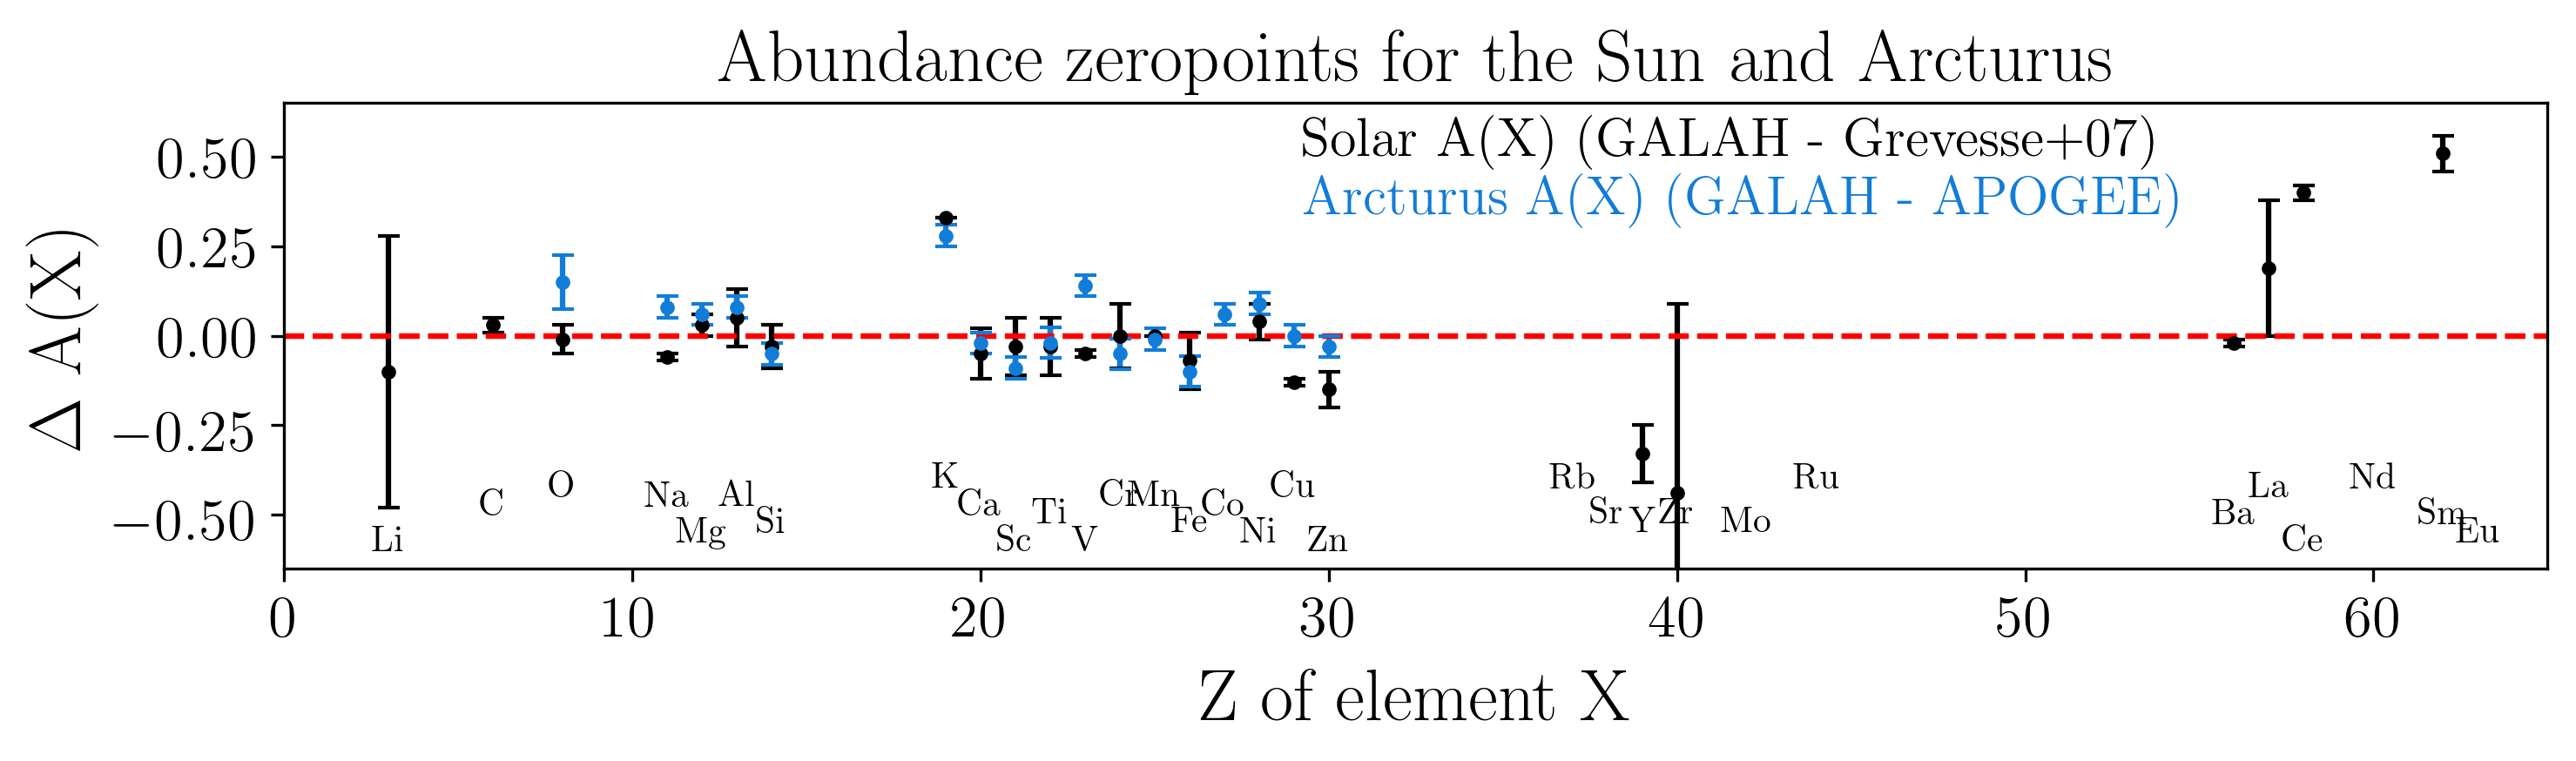
\includegraphics[width=\textwidth]{figures/old/abundance_zeropoints.png}
\caption[{Abundance offsets between the GALAH pipeline for a skyflat (150405000901378) and Arcturus (150210005801171).}]{Abundance offsets between GALAH pipeline for a skyflat (150405000901378) and Arcturus (150210005801171). Reference values are taken from \citet{Grevesse2007} and the APOGEE collaboration (priv. communication).}
\label{fig:abundance_zeropoints}
\end{figure*}

Final values: create script based on abundance\_zeropoints.ipynb, which creates a tex-table automatically:
see GALAH\_DR3\_abundances\_lines.tex and GALAH\_DR3\_Fe\_lines.tex in directory release\_paper/tables as well as validation/abundances
- solar abundances
- Arcturus abundances
- zeropoints are also saved in a FITS file. this is put into release\_paper/tables as well (galahdr3\_abundance\_zeropoints.fits)

\paragraph*{Abundances of the GBS stars}

\paragraph*{TBD: Abundances of cluster stars?}

\subsubsection{Precision of element abundances}

We assess the precision by comparing the internal SME covariance uncertainties with those from repeat observations of the same star in Fig.~\ref{fig:precision_ab}. Contrary to the stellar parameter estimation, we see that the covariance errors from the individual line measurements are in excellent agreement for almost all lines. The standard deviations of the measurements are also consistent irrespective of the fibre combination. In the chosen example of Si lines, only the Si line at $7680\,\mathrm{\AA}$  shows a slightly lower trend than the repeat observations. When combining the individual Si abundances to the error-weighted mean [Si/Fe], we see the expected improvement of precision down to $0.041\,\mathrm{dex}$ at $S/N = 40$ per pixel. We note however that the finally estimated internal SME-based errors are lower than the those from the repeat observations. This seems to illustrate that the SME-internal method has problems to estimate realistic errors when many pixels are involved, likely reflecting on the many imperfections of the models. Contrary to the stellar parameter estimation, we only report the final abundance error from the internal covariance error.

\begin{figure*}
\centering
\includegraphics[width=0.85\textwidth]{figures/old/repeat_uncertainties_silicon.pdf}
\caption[{Precision estimates from internal SME covariance for selected element abundances.}]{Precision estimates from internal SME covariance uncertainties (blue) as well as standard deviations from all (orange), same fibre (green), and different fibre (violet) repeat observations for the combined $\upalpha$-abundances (top left), the combined Si abundances (top right) as well as six individual Si lines.}
\label{fig:precision_ab}
\end{figure*}


\paragraph*{Abundances of repeat observations}

\paragraph*{TBD: Abundances of cluster stars?}

\subsection{The complexity and importance of flagging (and using them)}

\subsubsection{Flagging of stellar parameters}

After all stellar parameters have been estimated, the results are vetted and flags raised for the individual criteria listed in Table~\ref{tab:flag_sp_galah_dr3}. Fig.~\ref{fig:hrd_galah_dr3_not0} shows all those spectra with raised flags. It can be seen that our flagging algorithm is rather conservative, because the plot resembles Fig.~\ref{fig:hrd_galah_dr3} quite well. The most used flags are 8 (7\%), 1 (6\%) and 4 (3\%). 

\begin{figure*}
\centering
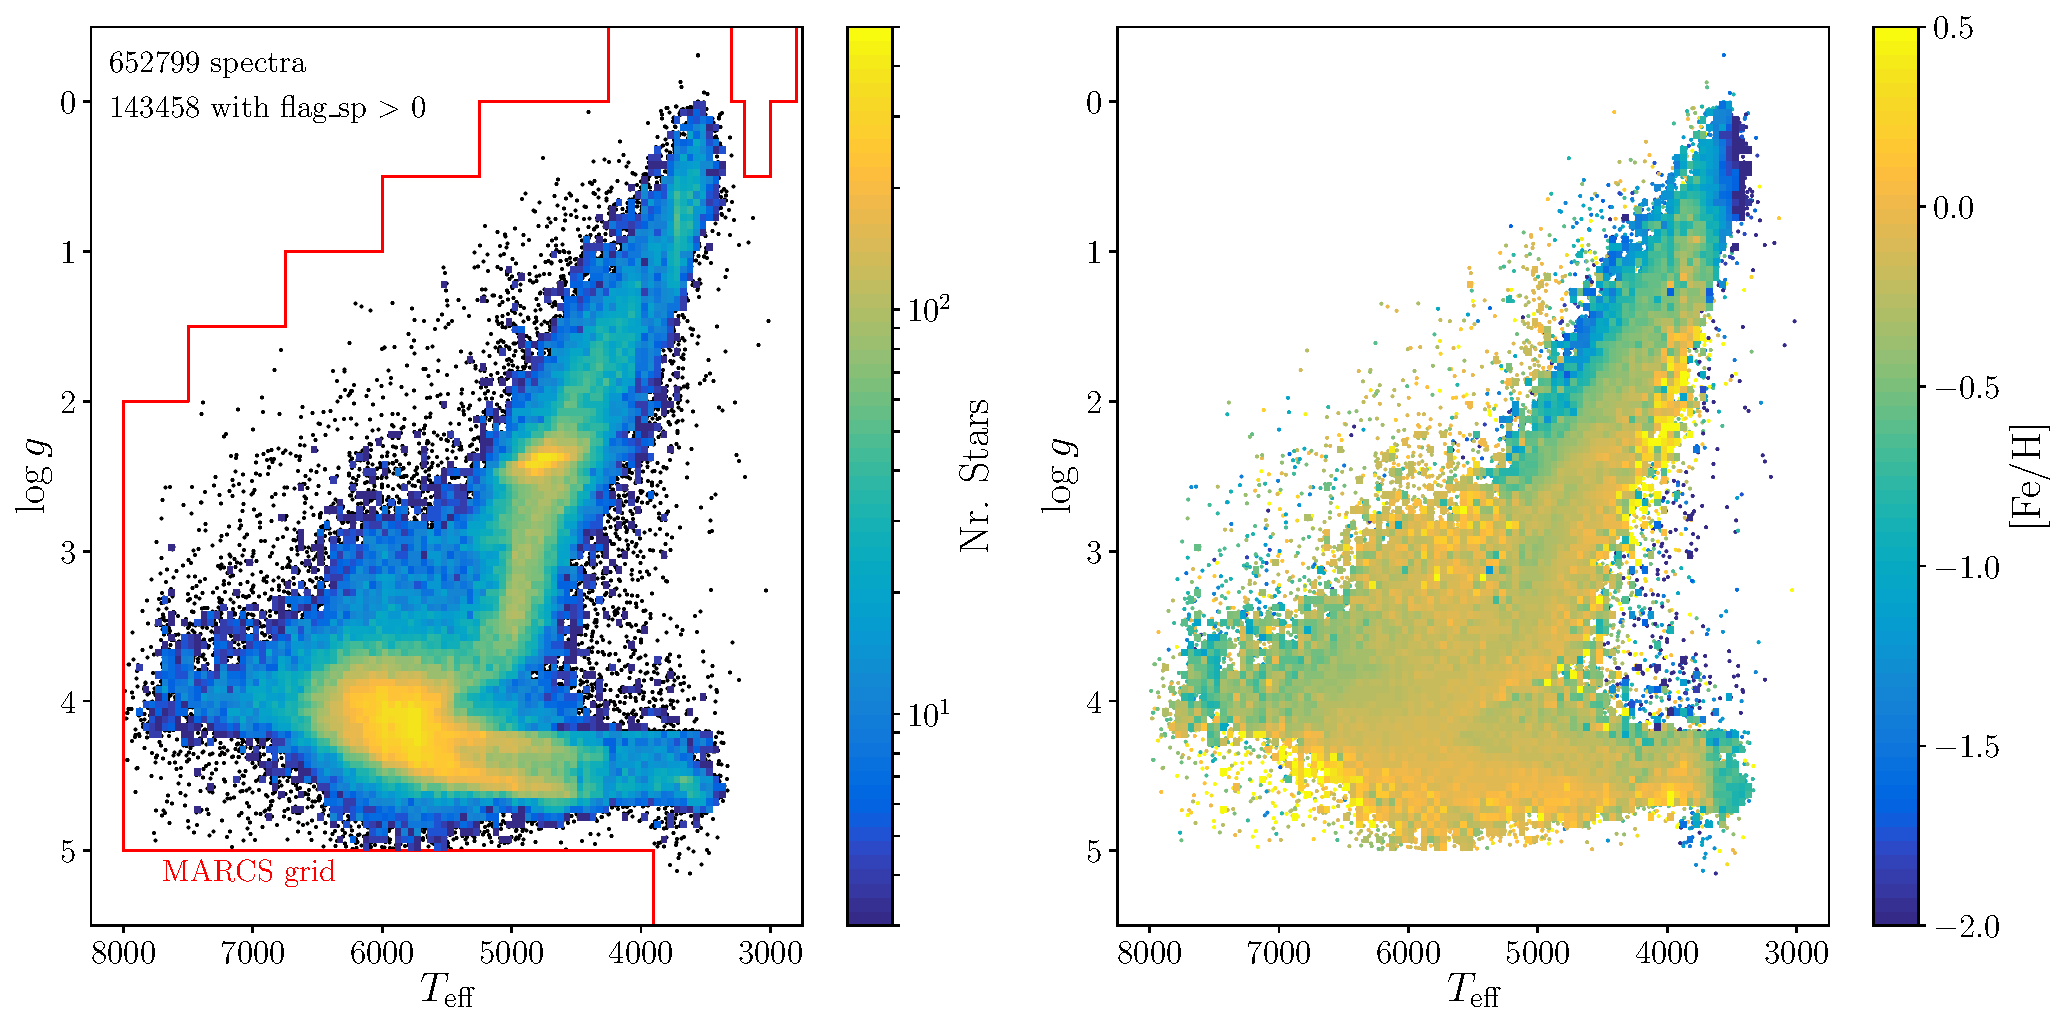
\includegraphics[width=\textwidth]{figures/old/Kiel_Diagram_GALAH_flag_not0.pdf}
\caption[{Kiel diagrams ($T_\text{eff}$ vs. $\log g$) color coded by the density of stars per bin (left panel) and mean iron abundance [Fe/H] within a bin (right panel) for those stars of the GALAH data release 3 at least have estimated stellar parameters, but have been flagged ($\texttt{flag\_sp} > 0$).}]{Kiel diagrams ($T_\text{eff}$ vs. $\log g$) color coded by the density of stars per bin (left panel) and mean iron abundance [Fe/H] within a bin (right panel) for those 129369 spectra of the GALAH data release 3 at least have estimated stellar parameters, but have been flagged ($\texttt{flag\_sp} > 0$), contrary to the unflagged spectra in Fig.~\ref{fig:hrd_galah_dr3}. The total number of spectra and those below the quality threshold are annotated in the upper left corner of the left panels. In the same panels, red lines indicate the grid limit of the MARCS atmosphere grid, which marks the limits of the synthesis computations.}
\label{fig:hrd_galah_dr3_not0}
\end{figure*}

We have identified astrometric binaries (\texttt{flag\_sp} = 64) by selecting the oldest isochrones for the particular iron abundance of each star and selecting all stars with surface gravity lower by $\Delta \log g = 0.15$ and cooler by $\Delta T_\text{eff} = 150\,\mathrm{K}$. This selection is most effective for the identification of binaries on the secondary main-sequence (with slightly lower $\log g$). For stars with equal bolometric luminosity, for example a binary system with the same stellar parameters, the estimated $\log g$ can be smaller by up to $\sim 0.3$. This deviation can be approximated via Eq.~\ref{eq:bolometric_logg} when assuming that the bolometric luminosity of the system is twice that of a single star and the mass is estimated to be that of a single star, so that $\Delta \log g \sim - \log L_\text{bol, binary} + \log L_\text{bol, single} = - \log \left( 2 \cdot L_\text{bol, single} \right) + \log L_\text{bol, single} = - \log 2 $. We have also identified unreliable parameter estimates for the coolest bright giants, for which unreasonably low iron abundances have been estimated (see tip of the RGB in right panel of Fig.~\ref{fig:hrd_galah_dr3_not0}).

\begin{table}
 \caption{Flags used for GALAH DR3 to estimate the final bit-flag \texttt{flag\_sp} via summation of the individual flags.}
 \label{tab:flag_sp_galah_dr3}
 \begin{tabular}{rl}
  \hline \hline
Flag		&	Description	\\
\hline
   1	&	\Gaia RUWE > 1.4 \\
   	&	\citep[bad astrometric solution, see][]{Lindegren2018b} \\
   2	&	Unreliable broadening \\
   4	&	Low S/N (10 for CCD 2) \\
   8	&	Reduction issues \\
	&	a) Wavelength solution (propagating of \texttt{red\_flag} ) \\
	&	b) t-SNE projected reduction issues: \\
	&	Negative/positive fluxes, spikes, etc. \\
  16	&	t-SNE projected emission features \\
  32	&	t-SNE projected binaries \\
  64	&	Binary sequence/pre-main sequence flag \\
 128	&	SNR-dependent high SME chi2 (bad fit) \\
 256	&	Problems with Fe lines, where line flux is \\
 	&	not between 0.03 and 1.00 \\
 512	&	SME did not finish \\
     	&	a) No convergence == non-finite stellar parameters \\
   	&	b) Gaussian RV fit failed \\
     	&	c) Timeout on ISAAC \\
1024	&	MARCS grid limit reached or \\
	&	outside of reasonable parameter range \\
  \hline
 \end{tabular}
\end{table}

\subsubsection{Flagging of element abundances}

We expect less trends without the influence of the training set selection or data-model flexibilities, but we still expect trends for several reasons:
\begin{itemize}
\item Given the model- and setup-imperfections, excluding \logg as a free fitting parameter might lead to systematic trends. This can be the case for those stars where the true \logg of the star and our estimated \logg differ significantly (e.g. binaries where the (unidentified) second component is contributing to the flux of the system) or the synthetic spectrum with the true \logg does not match the observation (e.g. due to shortcomings of the 1D model atmospheres and synthesis).
\item For stars with more lines, our pipeline will perform worse several ways. Firstly, estimating the continuum will be less reliable. Secondly, we will run into issues of strong blending, where our estimate is limited to how close the synthesis of the blending lines is to the true observation. If for example a star has scaled solar abundances, our estimates of the element abundances will still be good even for blended cases. If the compositions differs, and the line that we want to measure is blended by a line of a significantly over- or under-abundant element (relative to scaled-solar), our measurement might be corrupted. We try to limit this by performing a blending test, but setting the limit on how much blending is still acceptable is both non-trivial but also hard to flag during post-processing.
\item Due to time/computation restrictions, we were running several elements in a combined rather than line-by-line basis, which can decrease the precision as outlined in Sec.~\ref{sec:analysis_flow}, although we have tried to ensure that the abundance zero points of the individual lines were similar for those elements that were run with the combined setup.
\end{itemize}

\subsubsection{Expect the (un-)expected, but be cautious: Analysis shortcoming or physical correlation?}

\paragraph*{Am/Fm stars}

We and others (e.g. \citet{Xiang2020}) have found them and our pipeline estimates abundance patterns very \citet{Fossati2008}, see their Figs. 11 and 12.
However, we want to stress that our pipeline is not adjusted for the analysis of such stars, and our approach of assuming ionisation equilibrium might fail in these stars and their abundances might thus be wrongly measured.

\paragraph*{Isochrone choice for mass estimation} We could select better isochrone sets in terms of 1) finer sampling (especially for younger stars), 2) treatment of alpha-enhancement (expanding the isochrones by those which have been calculated with alpha-enhancement) 3) stellar physics treatment like atomic diffusion 4) age choices beyond the age of the universe (for more reliable age uncertainty estimates)

\paragraph*{Binarity}

Price-Whelan: \url{https://arxiv.org/pdf/2002.00014.pdf} We expect way more binaries for the hot stars (see their Fig. 5).

\paragraph*{Microturbulence} In the future it is worth to test implementing $v_\text{mic}$ as a free parameter or use the relations estimated by \citet{DutraFerreira2016} based on 3D atmosphere calculations. Whereas these agree with the empirical GALAH iDR3 relations for the majority of the stars within $20\%$, they differ significantly for the hottest and most luminous stars, for which GALAH iDR3 is currently not estimating the most reliable stellar parameters anyway.

Using $v_\text{mic}$ as a free parameter showed significant improvements of trends with $T_\text{eff}$ for the APOGEE survey \citep{Holtzman2018} and will be tested for the next data releases

\begin{figure*}
\centering
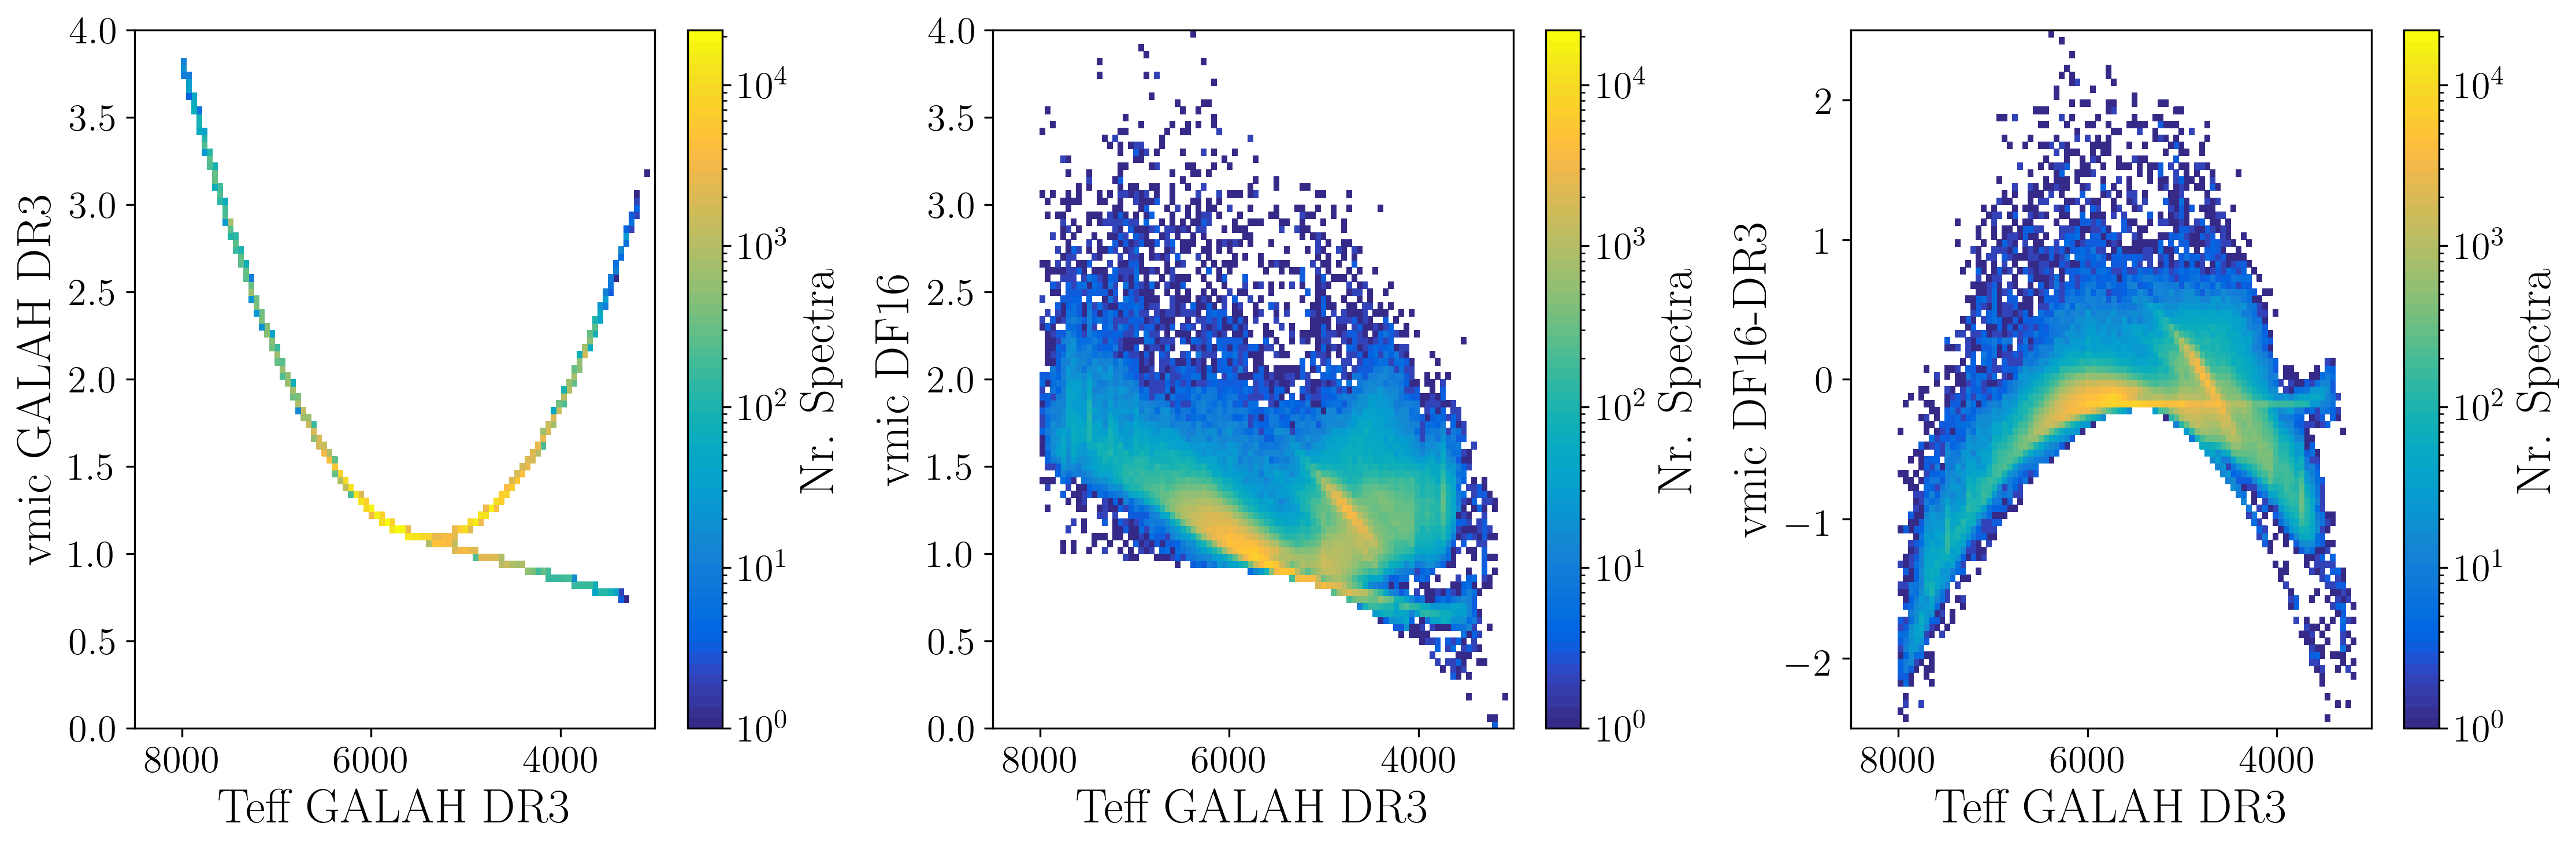
\includegraphics[width=\textwidth]{figures/Vmic_comparisons.png}
\caption[{Comparison of $v_\text{mic}$ calculated via relations used for GALAH iDR3 and \citet{DutraFerreira2016}}]{Relations of $v_\text{mic}$ as a function of $T_\text{eff}$ calculated via relations used for GALAH iDR3 and \citet{DutraFerreira2016} in the left and middle panels, respectively. A comparison of the two $v_\text{mic}$ values as a function of temperature is plotted in the right panel and shows good agreement for the majority of stars, i.e. cool and warm dwarfs and stars around the RC. However, the two relations disagree strongly for the most luminous and hottest stars. For the latter, GALAH iDR3 $v_\text{mic}$ values are up to two times higher.}
\label{fig:vmic_comparison}
\end{figure*}

\paragraph*{Metallicity trends in clusters} In clusters, we see a strong trend of temperature with metallicity. Could this be caused by our prescription of vmic? See paper by Bartella et al. (\url{https://arxiv.org/pdf/2001.03179.pdf}) who find that vmic is overestimated and thus [Fe/H] is underestimated when using Fe lines in clusters.

\paragraph*{Extinction} we could estimate $A_X$ via SED fitting rather than just relying on the RJCE method or $R_{K_s}$*E(B-V)

\paragraph*{Over-/underdensities around atmosphere grid points} Overdensities at 3500 and 4750..(250)..8000K. Underdensities below 4750

\paragraph*{Scattering in Potassium} Due to interstellar Potassium? include flagging (if not done for DR3) by checking expected equivalent width via $W = f(E(B-V))$ relation from \citet{Munari1997} High [K/Fe] especially for RC stars. Systematics or physical effect (does not seem to be correlated with high A(Li)?

\paragraph*{Cool RC end} This issue was identified via clumps in element abundances (e.g. two low [O/Fe] clumps) at the cool end of the RC. In this area, we might mis-identify RC stars as RGB stars due to a lack of appropriate RC clump isochrone entries. The underestimated mass might thus lead to an underestimated $\log g$.

\paragraph*{Stars with high extinction} Stars with high extinction will have uncertain logg. Flag them?

\paragraph*{Overdensity around 4650K, 4.7dex} Isochrone issue

\paragraph*{Noding in ages and masses} in ages due to chosen linear age grid 0.5..(0.5)..13.5 Gyr. This effects the hot stars and secondary RC. But why nodes in masses (for cool main sequence)

\paragraph*{Young star parameters} mass estimates possibly poor due to isochrone grid selection? vmic is not free, but tied to a relation. rotational broadening. Deviates strongly from true vmic? Line shape strongly influenced by activity?

\section{Catalogs included in this release}  \label{sec:catalogs}

%________________________________________________________________
\subsection{Main catalog} \label{sec:main_catalog}
\begin{enumerate}
\item Stellar paramaters (see Fig.~\ref{fig:hrd_galah_dr3})
\item Stellar parameter flags (both warning and flags)
\item Precision uncertainties and final uncertainties for each parameter (including accuracy, precision, and parameter node uncertainties)
\item Combined alpha-abundance (for unflagged measurements), see Fig.~\ref{fig:fe_h_alpha_fe}
\item Individual element abundances (including flagged measurements)
\item individual abundance flags
\item Precision uncertainties for each abundance
\item x-matches with Gaia DR2, Bailer-Jones2018, RUWE, 2MASS, WISE
\end{enumerate}

%________________________________________________________________
\subsection{Value-Added-Catalogs} \label{sec:value_added_catalogs}

The third Data Release of GALAH is accompanied by two value-added-catalogs and we explain them in this section. One value-added-catalog includes extended abundance measurement information, another one stellar ages as well as masses and a third one kinematic as well as dynamic information for each star.

\subsubsection{Extended abundance measurement information}

This VAC includes:
\begin{enumerate}
\item A(X) for each line of an element
\item Precision uncertainties for each abundance
\item flag for each line of an element
\item line flux estimates for each line of an element
\end{enumerate}

\subsubsection{Stellar age and mass estimates}

As part of the stellar parameter estimation (see Secs.~\ref{sec:3_applied_analyses}), both stellar masses and ages have been estimated and are added to the data release in a value-added-catalog. In Fig.~\ref{fig:mass_age_sanders}, we compare the mass and age difference to the study by \citet{Sanders2018}, who estimated both values based on GALAH DR2   as well as \Gaia DR2 in a Bayesian framework. We only compare those 215493 stars with \texttt{flag\_sp=0} from GALAH DR3 and  \texttt{flag=0} as well as \texttt{log10\_age>-1} (expected binaries) from \citet{Sanders2018} and find a good agreement between both analyses. For the masses we find an agreement in $\log_{10} (M)$ within 0.1 for 95\% of the stars and even within 0.05 for 82\% of the stars. The largest deviations are found both for massive stars (where GALAH masses are higher) and the metal-rich RC stars (where GALAH masses are lower). Regarding stellar ages we find a generally good agreement as well, with 73\% of the ages agreeing within 30\%. We note however, that especially for the young main-sequence and secondary RC stars  (on the GALAH scale), \citet{Sanders2018} tend to estimate even lower ages, whereas they estimate higher ages for cool main-sequence and metal-rich RC stars than our algorithm. Both regimes are prone to systematic trends, because the isochrone grids are very dense, that is tracks for very different masses and metallicities are very close.

\begin{figure*}
\centering
\includegraphics[width=0.49\textwidth]{figures/old/DS18_mass.pdf}
\includegraphics[width=0.49\textwidth]{figures/old/DS18_age.pdf}
  \caption[{Comparison of mass (left) and age (right) estimates from GALAH DR3 and \citet{Sanders2018}.}]{Comparison of mass (left) and age (right) estimates from GALAH DR3 and \citet{Sanders2018}.}
  \label{fig:mass_age_sanders}
\end{figure*}

We have further tested how well our algorithm can reproduce stellar ages from mock data, by selecting isochrone points of the 4 stellar ages (4.5, 8.0, 10.0, and $13.5\,\mathrm{Gyr}$), 4 different iron abundances ($\mathrm{[Fe/H]} \in [-2.0,-1.1,-.07,0.0]$), and 5 evolutionary stages, that is main-sequence ($T_\text{eff} \sim 5250\,\mathrm{K}$), turn-off (hottest around $\log g \sim 4.1$), RGB ($\log g \sim 3.25$), tip of the RGB ($\log g \sim 1.0$), and core helium burning RC (hottest for $2.0 < \log g < 3.0$). Each mock star is fed into the the mass and age estimation algorithm with generic uncertainties for the input parameters of $\Delta T_\text{eff} = 100\,\mathrm{K}$, $\Delta \log g = 0.5$, $\Delta \mathrm{[Fe/H]} = 0.2$, and $\Delta L_\text{bol} = 10\%$. We compare the retrieved age with the input age in Fig.~\ref{fig:Age_deviation_trends} and find that the age estimation tends to recover the stellar ages very well for turn-off stars as well as intermediate age stars around $8-10\,\mathrm{Gyr}$. For younger stars, the code tends to overestimate the age by up to $75\%$ for main-sequence stars and those at the tip of the RGB. The age of the oldest is typically underestimated, but RC and RGB star ages are better recovered than those of the tip of the RGB and the main-sequence. This means that the age of the oldest stars are typically underestimated and those of the youngest stars overestimated, resulting in an artificially tighter age distribution towards intermediate age stars. The code can, however, identify truly young stars and truly old stars.

\begin{figure*}
\centering
\includegraphics[width=\textwidth]{figures/old/Age_deviation_trends_rel.pdf}
  \caption[{Relative deviation of estimated stellar age from stellar ages as chosen from isochrone points.}]{Relative deviation of estimated stellar age from stellar ages as chosen from isochrone points at different $\mathrm{[Fe/H]} \in [-2.0, -1.1, -.07, 0.0]$ (as indicated in lower right of each panel), different stellar $\mathrm{ages} \in [4.5, 8.0, 10.0, 13.5]\,\mathrm{Gyr}$ (different bars with same colours as indicated by axis labels) and different evolutionary stages (different colours as indicated by plot legend in upper left panel).}
  \label{fig:Age_deviation_trends}
\end{figure*}

\subsubsection{Kinematic and dynamic information}

The second value-added-catalog includes coordinates as well as kinematic and dynamic information for each star. We use the astrometric information from \Gaia DR2 \citep{Brown2018}, that is \texttt{ra}, \texttt{dec}, \texttt{parallax} \citep[converted into distances by][]{BailerJones2018}, \texttt{pmra}, and \texttt{pmdec} as well as the radial velocities this third data release of the GALAH collaboration, that is  \texttt{rv\_galah}.

We use \textsc{galpy} \citep{Bovy2015} to transform these 6D information into the same Galactocentric reference frames (both cartesian and cylindrical) as stated in Table~\ref{tab:xyz_uvw}, that is with a circular velocity of $229.0\,\mathrm{km\,s^{-1}}$ \citep{Eilers2019}. We place the Sun at $R_\odot = 8.178\,\mathrm{kpc}$ \citep{Abuter2019} and $z_\odot = 0.025\,\mathrm{kpc}$ \citep{Juric2008} with a Solar motion relative to the local standard of rest of $(U_\odot,V_\odot,W_\odot) = (11.1, 12.24, 7.25)\,\mathrm{km\,s^{-1}}$ \citep{Schoenrich2010}.

The distribution in Galactocentric cylindrical coordinates ($R,z$) is shown in panel a) and a top view ($X,Y$) in panel b) of Fig.~\ref{fig:coords_overview}. The vast majority of targets are distributed within less than $4\,\mathrm{kpc}$ from the Sun and covers a large fraction of the disk. The distribution shows an asymmetry along $R$ as well as in the $(X,Y)$ plane due fact that the observations are carried out from Australia. Because of the target selection of the GALAH main program ($\vert b \vert > 10\,\mathrm{deg}$), no stars are observed close to the Galactic plane. We note, however, that GALAH DR3 includes also observations from TESS-HERMES, K2-HERMES, and several smaller projects that targeted the Galactic bulge and clusters. The distribution in the panel a) is hence also including observations with $\vert b \vert < 10\,\mathrm{deg}$ especially towards the Galactic center at ($R,z$) = 0. A combination of distance uncertainties and special targeting of clusters and K2/TESS fields is causing finger-of-god effects in both panels.

\begin{figure*}
\centering
\includegraphics[width=\textwidth]{figures/old/coords_overview_clean_all.png}
  \caption[{Overview of space information of GALAH DR3 with ($R,z$) in left panel and ($X,Y$) in right panel.}]{Overview of space information of GALAH DR3 with ($R,z$) in left panel and ($X,Y$) in right panel.}
  \label{fig:coords_overview}
\end{figure*}

The space velocities $(U,V,W)$ in the Galactocentric cartesian coordinate frame are shown in a Toomre diagram in panel a) of Fig.~\ref{fig:actions_overview}. Most of the stars observed as part of GALAH DR3 have disk-like kinematics similar to the local standard of rest, but an extension of stars with lower rotational velocity than the disk ($V \ll 0\,\mathrm{km\,s^{-1}}$) are shown and indicate that also several stars with halo-like kinematic properties are part of GALAH DR3.

\begin{figure*}
\centering
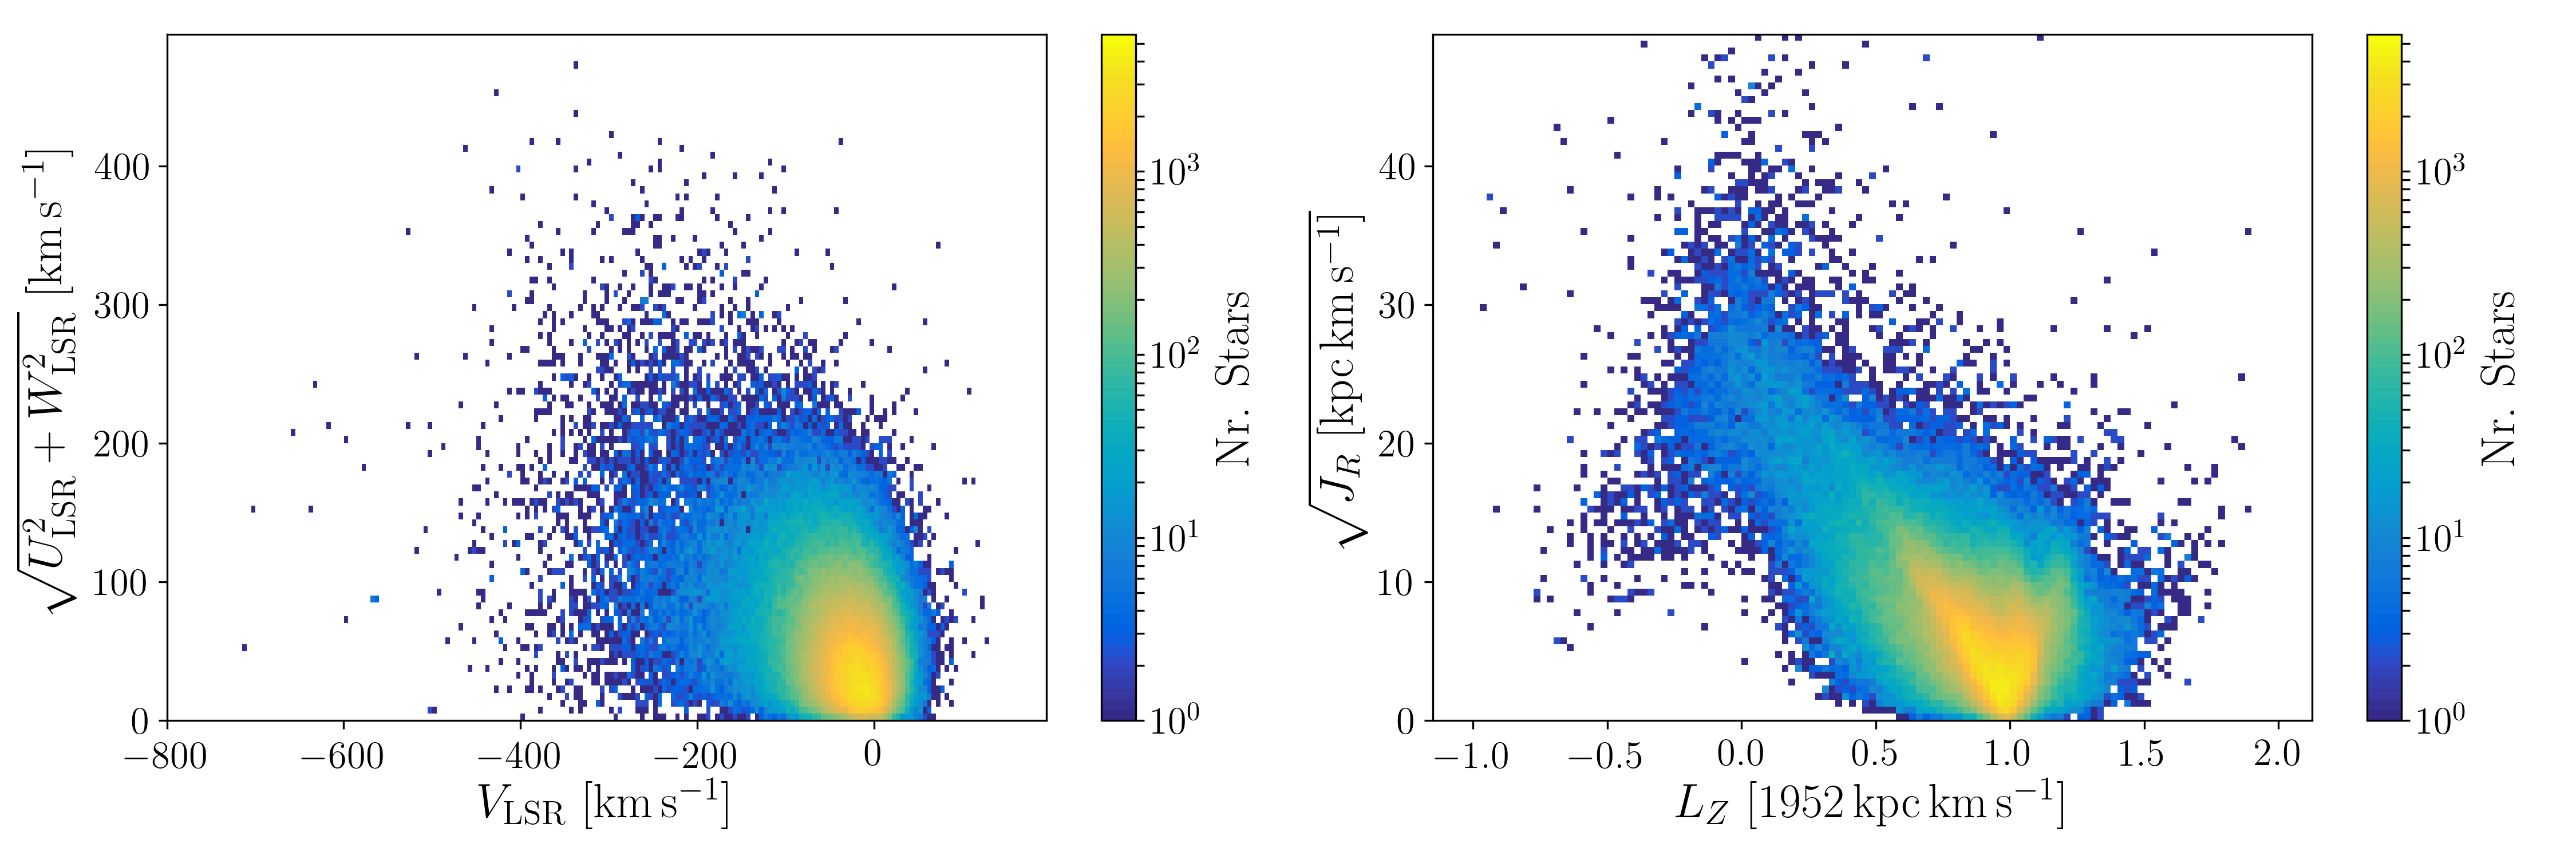
\includegraphics[width=\textwidth]{figures/old/action_overview_clean_all.png}
  \caption[{Overview of kinematic/dynamic information of GALAH DR3 with Toomre diagram (left) and Action diagram (right).}]{Overview of kinematic/dynamic information of GALAH DR3 with Toomre diagram (left) and Action diagram (right).}
  \label{fig:actions_overview}
\end{figure*}

We compute stellar dynamic properties, that is actions $J_R, L_z, J_z$, eccentricities $e$, and orbit boundary information such as $z_\text{max}$, $R_\text{peri}$, and $R_\text{apo}$ with \textsc{galpy} \citep{Bovy2015} in the \textsc{MWPotential2014} and a Staeckel fudge with 0.45 as focal length of confocal coordinate system.

The distribution of stars in action space is shown in a view of vertical angular momentum (normalised to the Solar value) and radial action in panel b) of Fig.~\ref{fig:actions_overview}. Most of the stars in this diagram show a similar vertical angular momentum radial action as the Sun. Similar to the analyses by \citet{Trick2019}, a rich substructure along $J_R$ can be seen. Similar to the extensions seen in the left panel of that figure, an extension of stars with lower vertical angular momentum is visible. We also note an overdensity close to $(L_Z,J_R) = (0,0)\,\mathrm{kpc\,km\,s^{-1}}$, that is an overdensity of stars with near-circular orbits close to the Galactic center and bulge. The overdensity of stars around $L_Z \sim 0 \,\mathrm{kpc\,km\,s^{-1}}$ with higher radial actions is typical for stars of the Galactic halo and is assessed in Chapter~\ref{sec:halo}.

For each of the computed phase space and dynamic properties, we report a variety of statistical values. In addition to the best-value, that is computed by using the best values as input, we also sample the distribution for each property within the uncertainties via Monte Carlo sampling with size 10000 and report the 5th, 50th, and 95th percentiles of these distributions. An example of the sampling of parameters for 100 randomly selected stars is shown in Fig.~\ref{fig:MC_output}.  We also provide the code to perform this sampling with different sampling choices. Whereas we currently sample the properties by assuming their input parameters are uncorrelated, we also provide the code to sample with the \Gaia correlation matrices. The latter are currently not applying a distance prior and are thus problematic for large distances. However, we stress, that the vast majority of the stars from GALAH DR3 have very precise parallax measurements, for which the sampling choice is negligible (see Fig.~\ref{fig:parallax_overview}).

\begin{figure*}
\centering
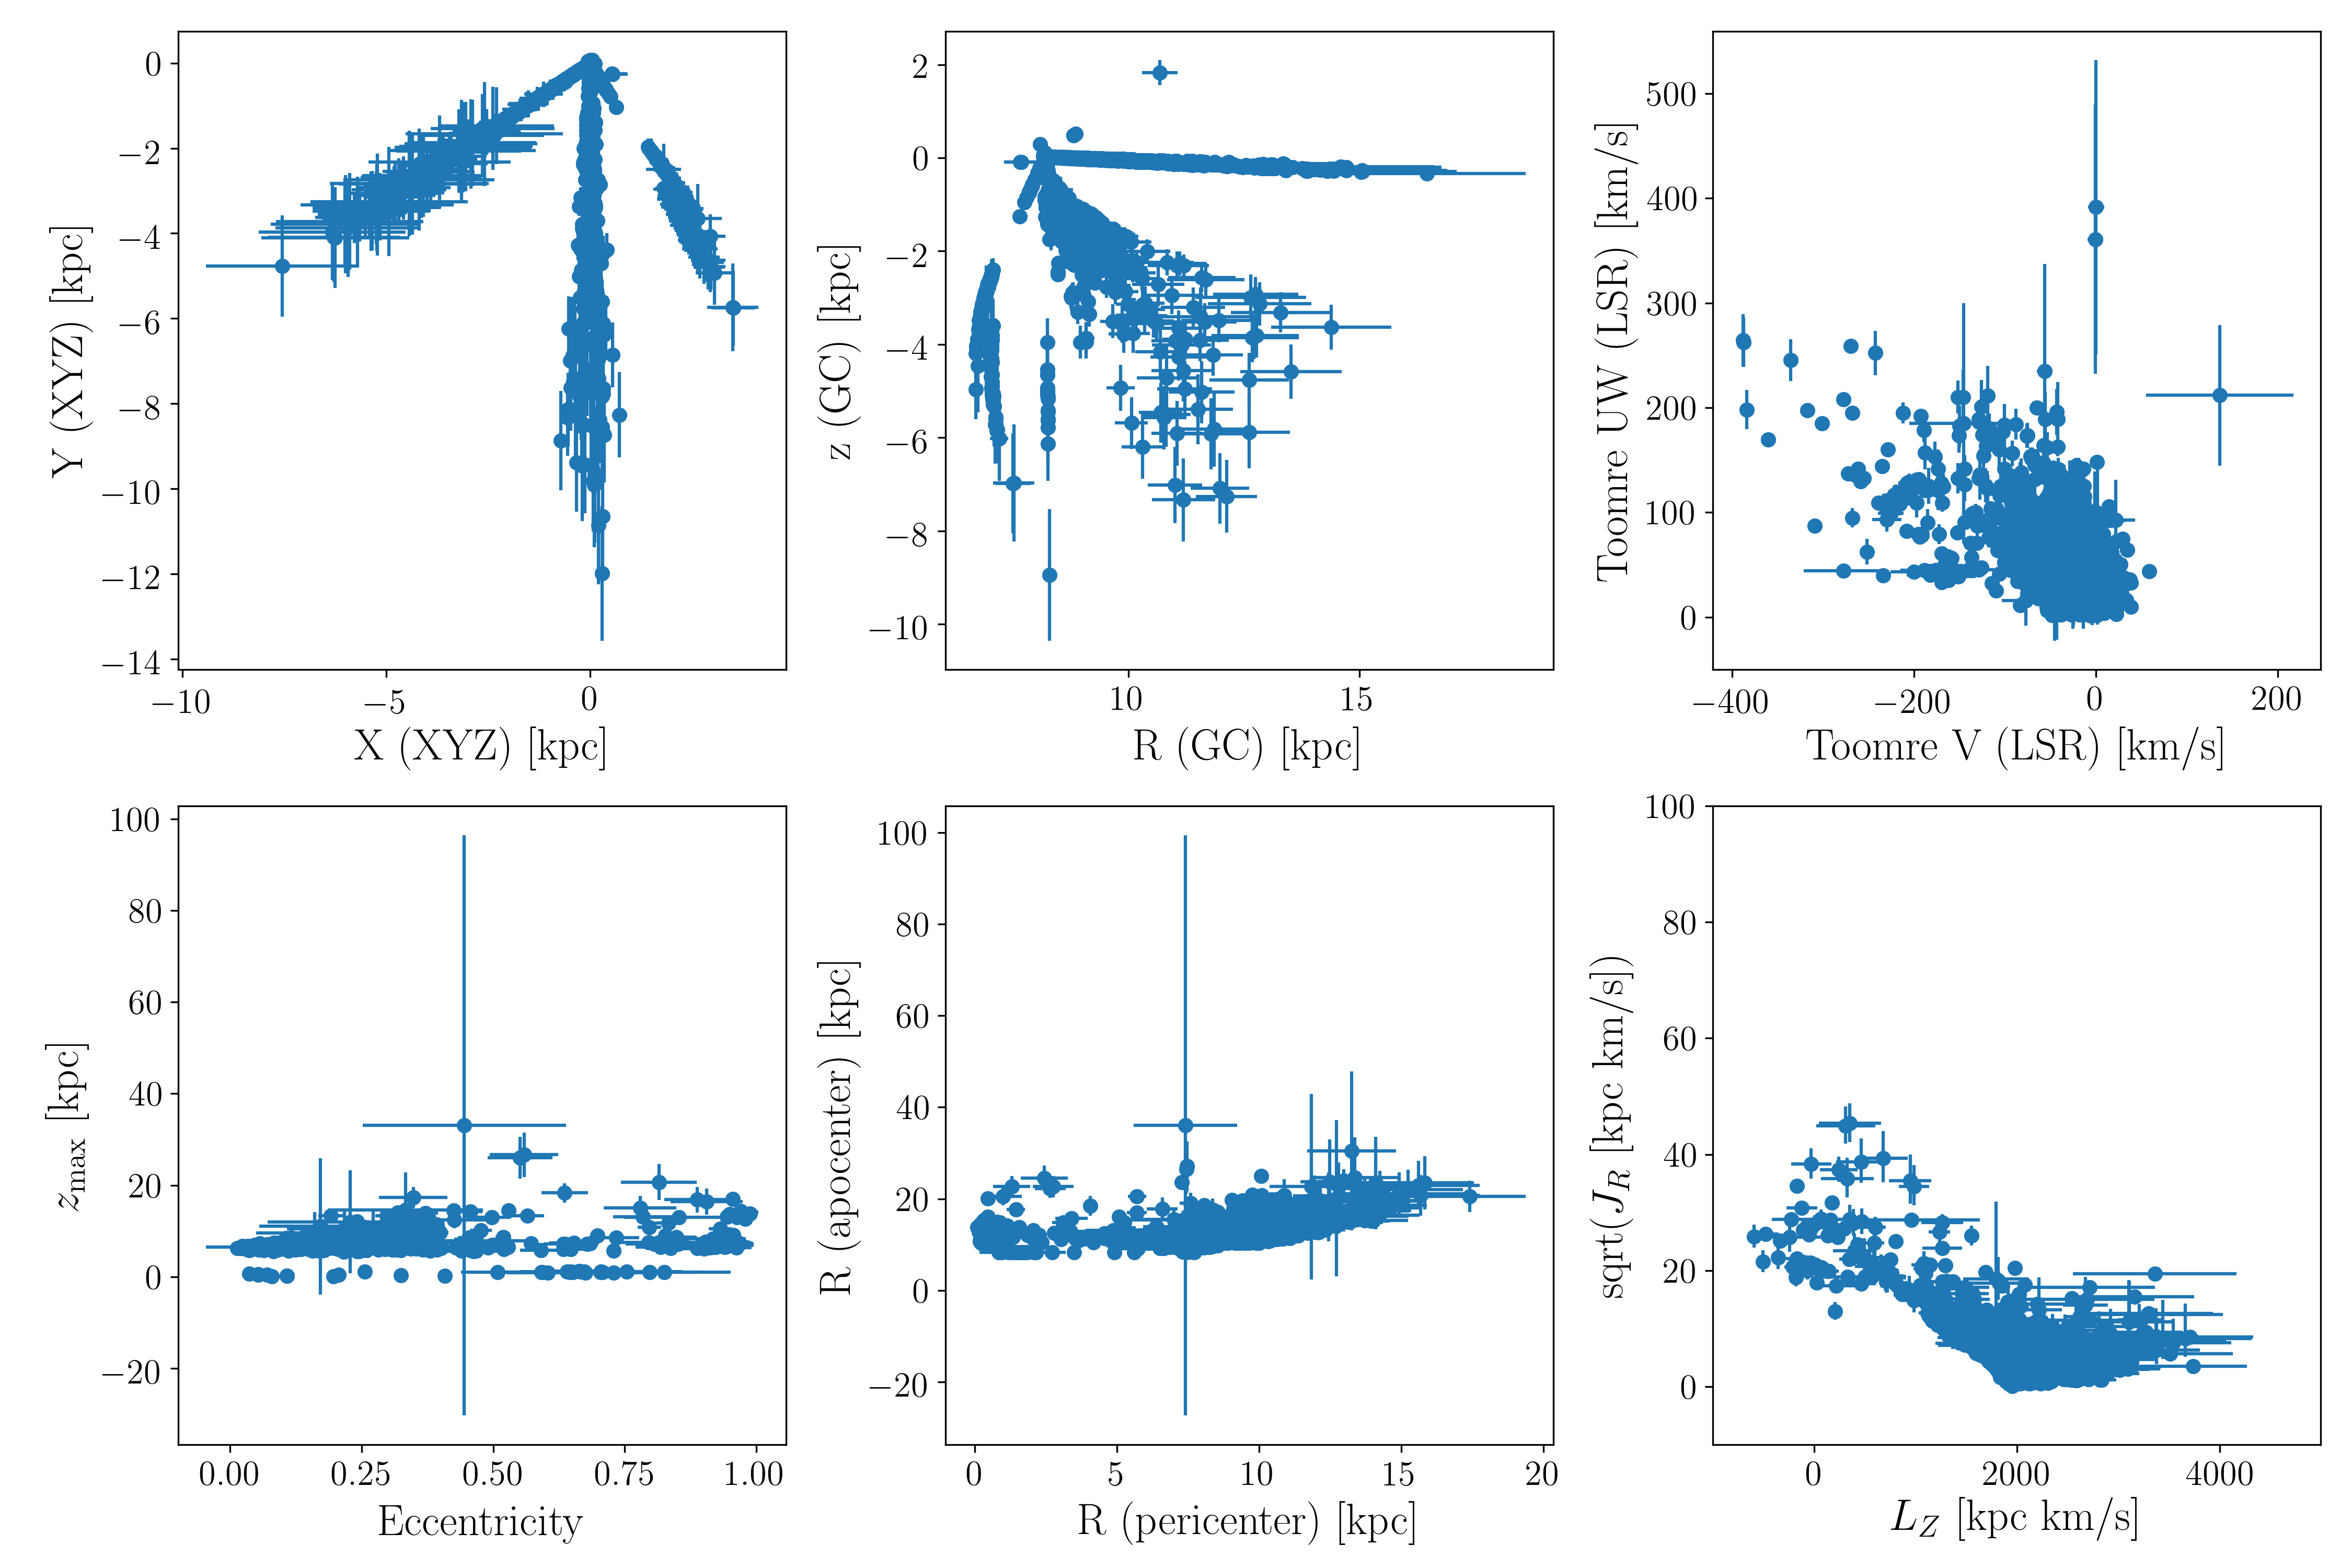
\includegraphics[width=\textwidth]{figures/old/MC_output.pdf}
  \caption[{Overview of phase space and dynamic stellar properties for randomly chosen stars from GALAH DR3, including their sampling within the measurement uncertainties.}]{Overview of phase space and dynamic stellar properties for randomly chosen stars from GALAH DR3, including their sampling within the measurement uncertainties. The black points indicate the values calculated from the best 6D information. Blue points indicate 10000 samples from the 6D information per star within the uncertainties. Red error bars indicate the distribution between 50th percentile (middle of the cross) and the 5th and 95th percentile, respectively.}
  \label{fig:MC_output}
\end{figure*}

%________________________________________________________________
\section{GALAH DR3 in context} \label{sec:galah_in_context}

\subsection{Galactic archaeology on a global scale}  \label{sec:global_ga}

\subsection{Chemodynamical evolution}  \label{sec:cde}

Combining chemistry, dynamics, and ages of stars

- plot Galactic $v_R$ vs. $v_\phi$ (Belokurov)
- plot Toomre diagram
- plot actions
- plot \cite{Vasiliev2019} overview of $J_i$

%________________________________________________________________
\section{Conclusions} \label{sec:conclusions}


%________________________________________________________________
\section*{Acknowledgements}

Based on data acquired through the Australian Astronomical Observatory, under programmes: A/2013B/13 (The GALAH pilot survey); A/2014A/25, A/2015A/19, A2017A/18 (The GALAH survey phase 1), A2018 A/18 (Open clusters with HERMES), A2019A/1 (Hierarchical star formation in Ori OB1),  A2019A/15 (The GALAH survey phase 2), A/2015B/19, A/2016A/22, A/2016B/10, A/2017B/16, A/2018B/15 (The HERMES-TESS program), and A/2015A/3, A/2015B/1, A/2015B/19, A/2016A/22, A/2016B/12, A/2017A/14, (The HERMES K2-follow-up program). \SB{Are we missing programs?} We acknowledge the traditional owners of the land on which the AAT stands, the Gamilaraay people, and pay our respects to elders past and present.

This work has made use of data from the European Space Agency (ESA) mission \Gaia (http://www.cosmos.esa.int/gaia), processed by the \Gaia Data Processing and Analysis Consortium (DPAC, http://www.cosmos.esa.int/web/gaia/dpac/consortium). Funding for the DPAC has been provided by national institutions, in particular the institutions participating in the \Gaia Multilateral Agreement. 

The following software and programming languages made this research possible: \textsc{IRAF} \citep{Tody1986,Tody1993}, \textsc{configure} \citep{Miszalski2006}, \textsc{topcat} \citep[version 4.4;][]{Taylor2005}; Python (version 2.7) and its packages {\textsc{astropy}} \citep[version 2.0;][]{Robitaille2013,PriceWhelan2018}, {\textsc{matplotlib}} \citep{matplotlib}, {\textsc{pandas}} \citep[version 0.20.2;][]{McKinney2011}, {\textsc{NumPy}} \citep{numpy}, {\textsc{IPython}} \citep{ipython}, and  \textsc{galpy} \citep[version 1.3;][]{Bovy2015}. This research has made use of the VizieR catalogue access tool, CDS, Strasbourg, France. The original description of the VizieR service was published in A\&AS 143, 23. This research mad use of the TOPCAT tool, described in \citet{Taylor2005}. This publication makes use of data products from the Two Micron All Sky Survey, which is a joint project of the University of Massachusetts and the Infrared Processing and Analysis Center/California Institute of Technology, funded by the National Aeronautics and Space Administration and the National Science Foundation.

SB and acknowledges funds from the Alexander von Humboldt Foundation in the framework of the Sofja Kovalevskaja Award endowed by the Federal Ministry of Education and Research. SB acknowledges travel support from Universities Australia and Deutsche Akademische Austauschdienst.

We would like to thank Chris Onken for crossmatching GALAH and SkyMapper DR3 data. \SB{Put SkyMapper REF here or up in the main text}

We would like to thank the SDSS and APOGEE collaboration for their efforts in documentation, which greatly benefited our efforts in documentation and validation.

%%%%%%%%%%%%%%%%%%%%%%%%%%%%%%%%%%%%%%%%%%%%%%%%%%

%%%%%%%%%%%%%%%%%%%% REFERENCES %%%%%%%%%%%%%%%%%%

% The best way to enter references is to use BibTeX:

\bibliographystyle{mnras}
\bibliography{bib} % if your bibtex file is called example.bib

%%%%%%%%%%%%%%%%%%%%%%%%%%%%%%%%%%%%%%%%%%%%%%%%%%

\newpage
\noindent \rule{8.5cm}{1pt}

\noindent
% List of institutions
$^{1}$Max Planck Institute  for Astronomy (MPIA), Koenigstuhl 17, 69117 Heidelberg, Germany\\
$^{2}$Research School of Astronomy \& Astrophysics, Australian National University, ACT 2611, Australia\\
$^{3}$Center of Excellence for Astrophysics in Three Dimensions (ASTRO-3D), Australia\\

%%%%%%%%%%%%%%%%% APPENDICES %%%%%%%%%%%%%%%%%%%%%

\appendix

\section{Linelist}\label{sec:linelist}

\begin{table*}
\caption{Selected lines for the elemental abundance analysis.}\label{linelist}
  \label{tab:linelist}
\centering
\begin{tabular}{l l l l l p{2.8cm} l l}
\hline
Elem. & Ion & Wavelength [\AA] & LEP [eV] & $\log(gf)$ & Reference & Line mask [\AA] & Segment mask [\AA] \\                                                                                            
\hline    
Li & 1 &6707.7635 & 0.00000 & -0.00200000 & 1998PhRvA..57.1652Y & 6707.3000-6708.3000 & 6705.76-6709.76 \\                                                                                              
Li & 1 &6707.9145 & 0.00000 & -0.303000 & 1998PhRvA..57.1652Y & 6707.3000-6708.3000 & 6705.76-6709.76 \\                                                                                                
Li & 1 &6707.9215 & 0.00000 & -0.00200000 & 1998PhRvA..57.1652Y & 6707.3000-6708.3000 & 6705.76-6709.76 \\                                                                                              
Li & 1 &6708.0725 & 0.00000 & -0.303000 & 1998PhRvA..57.1652Y & 6707.3000-6708.3000 & 6705.76-6709.76 \\                                                                                                
C  & 1 &6587.6100 & 8.53700 & -1.02100 & 1993A\&AS...99..179H & 6587.2610-6587.9860 & 6585.61-6589.61 \\                                                                                                
O  & 1 &7771.9440 & 9.14600 & 0.369000 & NIST & 7771.3590-7772.5090 & 7769.50-7777.50 \\                                                                                                                
O  & 1 &7774.1660 & 9.14600 & 0.223000 & NIST & 7773.5220-7774.7820 & 7769.50-7777.50 \\                                                                                                                
O  & 1 &7775.3880 & 9.14600 & 0.00200000 & NIST & 7774.9120-7775.9620 & 7769.50-7777.50 \\                                                                                                              
Na & 1 &5682.6333 & 2.10200 & -0.706000 & GESMCHF & 5682.5170-5682.9970 & 5680.63-5691.20 \\                                                                                                            
Na & 1 &5688.2050 & 2.10400 & -0.404000 & GESMCHF & 5687.9170-5688.3920 & 5680.63-5691.20 \\                                                                                                            
Mg & 1 &5711.0880 & 4.34600 & -1.72400 & 1990JQSRT..43..207C & 5710.7570-5711.4280 & 5710.00-5713.09 \\                                                                                                 
Al & 1 &6696.0230 & 3.14300 & -1.56900 & 2008JPCRD..37..709K & 6695.7780-6696.1730 & 6695.00-6699.87 \\                                                                                                 
Al & 1 &6698.6730 & 3.14300 & -1.87000 & 2008JPCRD..37..709K & 6698.3920-6698.8950 & 6695.00-6699.87 \\                                                                                                 
Al & 1 &7835.3090 & 4.02200 & -0.689000 & 2008JPCRD..37..709K & 7834.8840-7835.5720 & 7834.00-7837.50 \\                                                                                                
Al & 1 &7836.1340 & 4.02200 & -0.534000 & 2008JPCRD..37..709K & 7835.8130-7836.4310 & 7834.00-7837.50 \\                                                                                                
Al & 1 &7836.1340 & 4.02200 & -1.83400 & 2008JPCRD..37..709K & 7835.8130-7836.4310 & 7834.00-7837.50 \\                                                                                                 
Si & 1 &5684.4840 & 4.95400 & -1.55300 & GARZ|BL & 5684.1840-5684.7840 & 5683.00-5686.00 \\                                                                                                             
Si & 1 &5690.4250 & 4.93000 & -1.77300 & GARZ|BL & 5690.1800-5690.6830 & 5688.43-5692.43 \\                                                                                                             
Si & 1 &5701.1040 & 4.93000 & -1.95300 & GARZ|BL & 5700.9290-5701.2860 & 5699.70-5702.00 \\                                                                                                             
Si & 1 &5772.0272 & 5.61400 & -3.10700 & K07 & 5771.8460-5772.4460 & 5771.15-5773.15 \\                                                                                                                 
Si & 1 &5772.1460 & 5.08200 & -1.65300 & GARZ|BL & 5771.8460-5772.4460 & 5771.15-5773.15 \\                                                                                                             
Si & 1 &5793.0726 & 4.93000 & -1.96300 & GARZ|BL & 5792.7190-5793.3930 & 5791.07-5794.70 \\                                                                                                             
Si & 1 &6721.2732 & 5.96400 & -5.27200 & K07 & 6721.2000-6722.3000 & 6718.45-6723.85 \\                                                                                                                 
Si & 1 &6721.8481 & 5.86300 & -1.06200 & 1993PhyS...48..297N & 6721.2000-6722.3000 & 6718.45-6723.85 \\                                                                                                 
Si & 1 &7680.2660 & 5.86300 & -0.590000 & GARZ|BL & 7679.9440-7680.6680 & 7678.27-7682.27 \\                                                                                                            
K  & 1 &7698.9643 & 0.00000 & -0.178000 & 2017PhRvA..95e2507T & 7698.5730-7699.2960 & 7696.96-7700.96 \\                                                                                                

%Li & 1 &6707.7635 & 0.00000 & -0.00200000 & 1998PhRvA..57.1652Y & 6707.3000-6708.3000 & 6705.76-6709.76 \\                                                                                              
Li & 1 &6707.9145 & 0.00000 & -0.303000 & 1998PhRvA..57.1652Y & 6707.3000-6708.3000 & 6705.76-6709.76 \\                                                                                                
Li & 1 &6707.9215 & 0.00000 & -0.00200000 & 1998PhRvA..57.1652Y & 6707.3000-6708.3000 & 6705.76-6709.76 \\                                                                                              
Li & 1 &6708.0725 & 0.00000 & -0.303000 & 1998PhRvA..57.1652Y & 6707.3000-6708.3000 & 6705.76-6709.76 \\                                                                                                
C  & 1 &6587.6100 & 8.53700 & -1.02100 & 1993A\&AS...99..179H & 6587.2610-6587.9860 & 6585.61-6589.61 \\                                                                                                
O  & 1 &7771.9440 & 9.14600 & 0.369000 & NIST & 7771.3590-7772.5090 & 7769.50-7777.50 \\                                                                                                                
O  & 1 &7774.1660 & 9.14600 & 0.223000 & NIST & 7773.5220-7774.7820 & 7769.50-7777.50 \\                                                                                                                
O  & 1 &7775.3880 & 9.14600 & 0.00200000 & NIST & 7774.9120-7775.9620 & 7769.50-7777.50 \\                                                                                                              
Na & 1 &5682.6333 & 2.10200 & -0.706000 & GESMCHF & 5682.5170-5682.9970 & 5680.63-5691.20 \\                                                                                                            
Na & 1 &5688.2050 & 2.10400 & -0.404000 & GESMCHF & 5687.9170-5688.3920 & 5680.63-5691.20 \\                                                                                                            
Mg & 1 &5711.0880 & 4.34600 & -1.72400 & 1990JQSRT..43..207C & 5710.7570-5711.4280 & 5710.00-5713.09 \\                                                                                                 
Al & 1 &6696.0230 & 3.14300 & -1.56900 & 2008JPCRD..37..709K & 6695.7780-6696.1730 & 6695.00-6699.87 \\                                                                                                 
Al & 1 &6698.6730 & 3.14300 & -1.87000 & 2008JPCRD..37..709K & 6698.3920-6698.8950 & 6695.00-6699.87 \\                                                                                                 
Al & 1 &7835.3090 & 4.02200 & -0.689000 & 2008JPCRD..37..709K & 7834.8840-7835.5720 & 7834.00-7837.50 \\                                                                                                
Al & 1 &7836.1340 & 4.02200 & -0.534000 & 2008JPCRD..37..709K & 7835.8130-7836.4310 & 7834.00-7837.50 \\                                                                                                
Al & 1 &7836.1340 & 4.02200 & -1.83400 & 2008JPCRD..37..709K & 7835.8130-7836.4310 & 7834.00-7837.50 \\                                                                                                 
Si & 1 &5684.4840 & 4.95400 & -1.55300 & GARZ|BL & 5684.1840-5684.7840 & 5683.00-5686.00 \\                                                                                                             
Si & 1 &5690.4250 & 4.93000 & -1.77300 & GARZ|BL & 5690.1800-5690.6830 & 5688.43-5692.43 \\                                                                                                             
Si & 1 &5701.1040 & 4.93000 & -1.95300 & GARZ|BL & 5700.9290-5701.2860 & 5699.70-5702.00 \\                                                                                                             
Si & 1 &5772.0272 & 5.61400 & -3.10700 & K07 & 5771.8460-5772.4460 & 5771.15-5773.15 \\                                                                                                                 
Si & 1 &5772.1460 & 5.08200 & -1.65300 & GARZ|BL & 5771.8460-5772.4460 & 5771.15-5773.15 \\                                                                                                             
Si & 1 &5793.0726 & 4.93000 & -1.96300 & GARZ|BL & 5792.7190-5793.3930 & 5791.07-5794.70 \\                                                                                                             
Si & 1 &6721.2732 & 5.96400 & -5.27200 & K07 & 6721.2000-6722.3000 & 6718.45-6723.85 \\                                                                                                                 
Si & 1 &6721.8481 & 5.86300 & -1.06200 & 1993PhyS...48..297N & 6721.2000-6722.3000 & 6718.45-6723.85 \\                                                                                                 
Si & 1 &7680.2660 & 5.86300 & -0.590000 & GARZ|BL & 7679.9440-7680.6680 & 7678.27-7682.27 \\                                                                                                            
K  & 1 &7698.9643 & 0.00000 & -0.178000 & 2017PhRvA..95e2507T & 7698.5730-7699.2960 & 7696.96-7700.96 \\                                                                                                
Ca & 1 &5857.1962 & 5.30000 & -2.66500 & K07 & 5857.0180-5857.6250 & 5855.45-5859.45 \\                                                                                                                 
Ca & 1 &5857.4510 & 2.93300 & 0.240000 & S & 5857.0180-5857.6250 & 5855.45-5859.45 \\                                                                                                                   
Ca & 1 &5867.5620 & 2.93300 & -1.57000 & S & 5867.3000-5867.7000 & 5865.50-5869.80 \\                                                                                                                   
Ca & 1 &6493.7810 & 2.52100 & -0.109000 & SR & 6493.4650-6493.9930 & 6491.78-6501.65 \\                                                                                                                 
Ca & 1 &6493.8033 & 5.63200 & -4.55900 & K07 & 6493.4650-6493.9930 & 6491.78-6501.65 \\                                                                                                                 
Ca & 1 &6499.6500 & 2.52300 & -0.818000 & SR & 6499.3780-6499.9550 & 6491.78-6501.65 \\                                                                                                                 
Sc & 1 &4743.8300 & 1.44800 & 0.422000 & LD & 4743.5490-4744.0000 & 4741.83-4746.83 \\                                                                                                                  
Sc & 1 &4753.1610 & 0.00000 & -1.65900 & LD & 4753.0000-4753.4000 & 4751.30-4755.50 \\                                                                                                                  
Sc & 2 &5657.8960 & 1.50700 & -0.603000 & LD & 5657.6780-5658.1220 & 5655.90-5659.90 \\                                                                                                                 
Sc & 2 &5667.1490 & 1.50000 & -1.30900 & LD & 5666.9060-5667.3230 & 5665.15-5669.15 \\                                                                                                                  
Sc & 1 &5671.7751 & 1.44800 & -0.505000 & LD & 5671.6050-5672.0920 & 5669.82-5673.82 \\                                                                                                                 
Sc & 1 &5671.7898 & 1.44800 & -0.209000 & LD & 5671.6050-5672.0920 & 5669.82-5673.82 \\                                                                                                                 
Sc & 1 &5671.8032 & 1.44800 & -0.471000 & LD & 5671.6050-5672.0920 & 5669.82-5673.82 \\                                                                                                                 
Sc & 1 &5671.8163 & 1.44800 & -0.290000 & LD & 5671.6050-5672.0920 & 5669.82-5673.82 \\                                                                                                                 
Sc & 1 &5671.8271 & 1.44800 & -1.02700 & LD & 5671.6050-5672.0920 & 5669.82-5673.82 \\                                                                                                                  
Sc & 1 &5671.8436 & 1.44800 & -0.232000 & LD & 5671.6050-5672.0920 & 5669.82-5673.82 \\                                                                                                                 
Sc & 1 &5671.8641 & 1.44800 & -0.178000 & LD & 5671.6050-5672.0920 & 5669.82-5673.82 \\                                                                                                                 
Sc & 1 &5717.3070 & 1.44000 & -0.532000 & LD & 5717.0000-5717.5000 & 5715.50-5719.50 \\                                                                                                                 
Sc & 1 &5724.1070 & 1.43300 & -0.661000 & LD & 5723.8940-5724.2690 & 5722.11-5726.11 \\                                                                                                                 
Sc & 2 &6604.6010 & 1.35700 & -1.30900 & LD & 6604.4090-6604.9790 & 6602.60-6606.60 \\                                                                                                                  
Ti & 1 &4758.1178 & 2.24900 & 0.510000 & LGWSC & 4757.9470-4758.3060 & 4756.12-4760.12 \\                                                                                                               
Ti & 1 &4759.1416 & 2.77800 & -3.00200 & K10 & 4759.0880-4759.4910 & 4756.12-4760.12 \\                                                                                                                 
Ti & 1 &4759.2697 & 2.25600 & 0.590000 & LGWSC & 4759.0880-4759.4910 & 4756.12-4760.12 \\                                                                                                               
Ti & 1 &4778.2547 & 2.23600 & -0.350000 & LGWSC & 4778.0790-4778.4420 & 4776.25-4780.00 \\                                                                                                              
Ti & 1 &4781.7106 & 0.848000 & -1.95000 & LGWSC & 4781.5730-4781.9310 & 4780.50-4782.76 \\                                                                                                              
Ti & 1 &4797.9757 & 2.33400 & -0.630000 & LGWSC & 4797.8350-4798.1290 & 4796.33-4799.41 \\                                                                                                              
Ti & 1 &4801.9016 & 0.818000 & -3.06000 & LGWSC & 4801.8000-4802.2000 & 4800.00-4803.90 \\                                                                                                              
Ti & 1 &4801.9486 & 0.826000 & -3.16000 & LGWSC & 4801.8000-4802.2000 & 4800.00-4803.90 \\                                                                                                              
Ti & 1 &4802.1370 & 2.24900 & -3.84500 & K10 & 4801.8000-4802.2000 & 4800.00-4803.90 \\                                                                                                                 
Ti & 1 &4820.2488 & 3.70900 & -5.44900 & K10 & 4820.0880-4820.6700 & 4818.41-4822.41 \\                                                                                                                 
Ti & 2 &4820.3706 & 5.90500 & -2.03700 & K10 & 4820.0880-4820.6700 & 4818.41-4822.41 \\                                                                                                                 
Ti & 1 &4820.4094 & 1.50300 & -0.380000 & LGWSC & 4820.0880-4820.6700 & 4818.41-4822.41 \\                                                                                                              
Ti & 1 &5689.4600 & 2.29700 & -0.360000 & NWL & 5689.2640-5689.8050 & 5687.46-5691.46 \\                                                                                                                
Ti & 1 &5716.4500 & 2.29700 & -0.720000 & NWL & 5716.2320-5716.8300 & 5714.45-5718.45 \\                                                                                                                
Ti & 1 &5716.7175 & 3.42400 & -3.00600 & K10 & 5716.2320-5716.8300 & 5714.45-5718.45 \\                                                                                                                 
Ti & 1 &5720.4359 & 2.29200 & -0.900000 & MFW & 5720.2450-5720.6750 & 5718.50-5722.50 \\                                                                                                                
Ti & 1 &5720.6453 & 3.29400 & -2.80700 & K10 & 5720.2450-5720.6750 & 5718.50-5722.50 \\                                                                                                                 
Ti & 1 &5739.4690 & 2.24900 & -0.610000 & LGWSC & 5739.2500-5739.7000 & 5737.47-5741.47 \\                                                                                                              
Ti & 1 &5866.3679 & 3.30500 & -1.05500 & K10 & 5866.0000-5866.8090 & 5864.79-5868.60 \\                                                                                                                 
Ti & 1 &5866.4513 & 1.06700 & -0.790000 & LGWSC & 5866.0000-5866.8090 & 5864.79-5868.60 \\                                                                                                              
Ti & 2 &5866.6643 & 8.08900 & -0.695000 & K10 & 5866.0000-5866.8090 & 5864.79-5868.60 \\                                                                                                                
Ti & 1 &5866.8072 & 3.32300 & -2.21300 & K10 & 5866.0000-5866.8090 & 5864.79-5868.60 \\                                                                                                                 
Ti & 1 &6599.1048 & 0.900000 & -2.02900 & 1983MNRAS.204..883B|1989A\&A...208..157G & 6598.8980-6599.4980 & 6597.11-6601.11 \\                                                                           
Ti & 1 &6716.6660 & 2.48800 & -1.37000 & LGWSC & 6716.4890-6716.9050 & 6714.67-6718.67 \\                                                                                                               
Ti & 1 &7852.6770 & 0.848000 & -2.64000 & BLNP & 7852.2000-7852.9970 & 7851.36-7854.67 \\                                                                                                               
Ti & 1 &7852.6819 & 1.87900 & -4.09600 & K10 & 7852.2000-7852.9970 & 7851.36-7854.67 \\                                                                                                                 
Ti & 1 &4719.3556 & 0.813000 & -4.45900 & K10 & 4719.3000-4719.6000 & 4719.00-4721.51 \\                                                                                                                
Ti & 2 &4719.5109 & 1.24300 & -3.32000 & WLSC & 4719.3000-4719.6000 & 4719.00-4721.51 \\                                                                                                                
Ti & 2 &4764.5247 & 1.23700 & -2.69000 & WLSC & 4764.3970-4764.8000 & 4762.52-4766.52 \\                                                                                                                
Ti & 2 &4798.5313 & 1.08000 & -2.66000 & WLSC & 4798.3300-4798.6440 & 4796.33-4799.41 \\                                                                                                                
Ti & 2 &4849.1678 & 1.13100 & -2.96000 & WLSC & 4849.0500-4849.4000 & 4847.17-4851.17 \\                                                                                                                
Ti & 2 &4865.6104 & 1.11600 & -2.70000 & WLSC & 4865.3000-4865.8500 & 4863.61-4867.61 \\                                                                                                                
Ti & 1 &4865.7808 & 2.57800 & -2.00000 & MA-astro & 4865.3000-4865.8500 & 4863.61-4867.61 \\                                                                                                            
Ti & 2 &4874.0094 & 3.09500 & -0.860000 & WLSC & 4873.8700-4874.1940 & 4872.01-4876.01 \\                                                                                                               
V  & 1 &4831.6457 & 0.0170000 & -1.38000 & 2014ApJS..215...20L & 4831.5250-4831.7290 & 4829.65-4833.65 \\                                                                                               
V  & 1 &4784.4665 & 0.0170000 & -2.67000 & 2014ApJS..215...20L & 4784.3360-4784.6070 & 4782.47-4786.47 \\                                                                                               
V  & 1 &4796.9140 & 2.09700 & 0.190000 & 2014ApJS..215...20L & 4796.7600-4796.9750 & 4794.91-4798.91 \\                                                                                                 
Cr & 1 &4775.1300 & 3.55100 & -1.05000 & MFW & 4774.9500-4775.3070 & 4773.13-4777.13 \\                                                                                                                 
Cr & 1 &4789.3350 & 2.54400 & -0.330000 & SLS & 4789.1930-4789.4820 & 4787.33-4791.33 \\                                                                                                                
Cr & 1 &4801.0247 & 3.12200 & -0.131000 & MFW & 4800.8390-4801.2330 & 4799.02-4803.02 \\                                                                                                                
Cr & 1 &5787.9190 & 3.32200 & -0.0830000 & MFW & 5787.6400-5788.1600 & 5786.32-5790.42 \\                                                                                                               
Cr & 1 &6630.0100 & 1.03000 & -3.56000 & MFW & 6629.7740-6630.2720 & 6627.51-6632.51 \\                                                                                                                 
Mn & 1 &4738.9176 & 3.77200 & -3.89500 & K07 & 4738.8970-4739.3040 & 4737.09-4741.09 \\                                                                                                                 
Mn & 1 &4739.0900 & 2.94100 & -0.604000 & DLSSC & 4738.8970-4739.3040 & 4737.09-4741.09 \\                                                                                                              
Mn & 1 &4753.8969 & 5.21400 & -0.920000 & K07 & 4753.8000-4754.3000 & 4752.04-4755.60 \\                                                                                                                
Mn & 1 &4754.0183 & 2.28200 & -0.647000 & DLSSC & 4753.8000-4754.3000 & 4752.04-4755.60 \\                                                                                                              
Mn & 1 &4754.0301 & 2.28200 & -0.787000 & DLSSC & 4753.8000-4754.3000 & 4752.04-4755.60 \\                                                                                                              
Mn & 1 &4754.0472 & 2.28200 & -0.668000 & DLSSC & 4753.8000-4754.3000 & 4752.04-4755.60 \\                                                                                                              
Mn & 2 &4754.0558 & 6.13900 & -3.12400 & K09 & 4753.8000-4754.3000 & 4752.04-4755.60 \\                                                                                                                 
Mn & 1 &4754.0635 & 2.28200 & -0.670000 & DLSSC & 4753.8000-4754.3000 & 4752.04-4755.60 \\                                                                                                              
Mn & 1 &4754.0784 & 2.28200 & -1.84000 & DLSSC & 4753.8000-4754.3000 & 4752.04-4755.60 \\                                                                                                               
Mn & 1 &4761.4912 & 2.95300 & -1.16600 & DLSSC & 4761.3520-4761.7620 & 4759.51-4763.51 \\                                                                                                               
Mn & 1 &4761.5060 & 2.95300 & -0.548000 & DLSSC & 4761.3520-4761.7620 & 4759.51-4763.51 \\                                                                                                              
Mn & 1 &4761.5198 & 2.95300 & -0.821000 & DLSSC & 4761.3520-4761.7620 & 4759.51-4763.51 \\                                                                                                              
Mn & 1 &4761.5408 & 2.95300 & -1.61300 & DLSSC & 4761.3520-4761.7620 & 4759.51-4763.51 \\                                                                                                               
Mn & 1 &4765.8380 & 2.94100 & -0.601000 & DLSSC & 4765.7110-4766.0570 & 4763.85-4767.85 \\                                                                                                              
Mn & 1 &4765.8525 & 2.94100 & -0.445000 & DLSSC & 4765.7110-4766.0570 & 4763.85-4767.85 \\                                                                                                              
Mn & 1 &4765.8647 & 2.94100 & -0.676000 & DLSSC & 4765.7110-4766.0570 & 4763.85-4767.85 \\                                                                                                              
Mn & 1 &4766.0086 & 4.42500 & -3.05400 & K07 & 4765.7110-4766.0570 & 4763.85-4767.85 \\                                                                                                                 
Fe & 1 &4788.7566 & 3.23700 & -1.76300 & BWL & 4788.5550-4788.9960 & 4787.50-4790.00 \\                                                                                                                 
Fe & 1 &4788.7786 & 4.14300 & -2.52300 & K14 & 4788.5550-4788.9960 & 4787.50-4790.00 \\                                                                                                                 
Fe & 1 &4793.9614 & 3.04700 & -3.43000 & MRW & 4793.8310-4794.1490 & 4792.80-4795.50 \\                                                                                                                 
Fe & 1 &4794.3541 & 2.42400 & -3.95000 & MRW & 4794.2370-4794.5460 & 4792.80-4795.50 \\                                                                                                                 
Fe & 1 &4802.8746 & 3.69500 & -2.02800 & K14 & 4802.6740-4803.0860 & 4801.70-4804.10 \\                                                                                                                 
Fe & 1 &4802.8797 & 3.64200 & -1.51000 & BWL & 4802.6740-4803.0860 & 4801.70-4804.10 \\                                                                                                                 
Fe & 1 &4803.0294 & 5.06400 & -2.94700 & K07 & 4802.6740-4803.0860 & 4801.70-4804.10 \\                                                                                                                 
Fe & 1 &4808.1478 & 3.25100 & -2.69000 & MRW & 4807.9950-4808.3280 & 4807.00-4809.30 \\                                                                                                                 
Fe & 1 &4875.8770 & 3.33200 & -1.90000 & 2014MNRAS.441.3127R & 4875.7500-4876.1000 & 4874.75-4877.10 \\                                                                                                 
Fe & 2 &4889.6227 & 0.0480000 & -8.09900 & K13 & 4889.5000-4890.9990 & 4888.50-4893.50 \\                                                                                                               
Fe & 2 &4889.6848 & 7.98800 & -3.75500 & RU & 4889.5000-4890.9990 & 4888.50-4893.50 \\                                                                                                                  
Fe & 2 &4889.7133 & 0.107000 & -14.0240 & K13 & 4889.5000-4890.9990 & 4888.50-4893.50 \\                                                                                                                
Fe & 2 &4889.7133 & 0.107000 & -12.1940 & K13 & 4889.5000-4890.9990 & 4888.50-4893.50 \\                                                                                                                
Fe & 1 &4889.7740 & 3.63400 & -9.84800 & K14 & 4889.5000-4890.9990 & 4888.50-4893.50 \\                                                                                                                 
Fe & 1 &4890.5192 & 4.30100 & -3.84600 & K14 & 4889.5000-4890.9990 & 4888.50-4893.50 \\                                                                                                                 
Fe & 1 &4890.7551 & 2.87600 & -0.386000 & BWL+2014MNRAS.441.3127R & 4889.5000-4890.9990 & 4888.50-4893.50 \\                                                                                            
Fe & 1 &4890.8477 & 4.54900 & -5.09400 & K14 & 4889.5000-4890.9990 & 4888.50-4893.50 \\                                                                                                                 
Fe & 1 &4890.9101 & 4.22000 & -2.45000 & K14 & 4889.5000-4890.9990 & 4888.50-4893.50 \\                                                                                                                 
Fe & 1 &4890.9620 & 4.58400 & -4.91200 & K14 & 4889.5000-4890.9990 & 4888.50-4893.50 \\                                                                                                                 
Fe & 1 &4891.4921 & 2.85100 & -0.111000 & BWL & 4891.2570-4892.5000 & 4888.50-4893.50 \\                                                                                                                
Fe & 1 &4891.7573 & 4.47300 & -5.09500 & K14 & 4891.2570-4892.5000 & 4888.50-4893.50 \\                                                                                                                 
Fe & 2 &4892.2622 & 6.70300 & -3.06800 & RU & 4891.2570-4892.5000 & 4888.50-4893.50 \\                                                                                                                  
Fe & 1 &5651.4689 & 4.47300 & -1.90000 & MRW & 5651.3150-5651.6460 & 5650.30-5653.50 \\                                                                                                                 
Fe & 2 &5651.5235 & 10.6290 & -0.615000 & RU & 5651.3150-5651.6460 & 5650.30-5653.50 \\                                                                                                                 
Fe & 1 &5651.5251 & 4.44600 & -4.76100 & K07 & 5651.3150-5651.6460 & 5650.30-5653.50 \\                                                                                                                 
Fe & 2 &5651.6338 & 10.6290 & -1.01000 & RU & 5651.3150-5651.6460 & 5650.30-5653.50 \\                                                                                                                  
Fe & 1 &5652.3176 & 4.26000 & -1.85000 & MRW & 5652.1100-5652.5330 & 5650.30-5653.50 \\                                                                                                                 
Fe & 1 &5661.2361 & 4.79500 & -3.94200 & K14 & 5661.1640-5661.6530 & 5660.20-5663.70 \\                                                                                                                 
Fe & 1 &5661.2813 & 4.19100 & -3.50100 & K14 & 5661.1640-5661.6530 & 5660.20-5663.70 \\                                                                                                                 
Fe & 1 &5661.3447 & 4.28400 & -1.75600 & BK & 5661.1640-5661.6530 & 5660.20-5663.70 \\                                                                                                                  
Fe & 1 &5662.5161 & 4.17800 & -0.447000 & BWL+GESHRL14 & 5662.3000-5662.7000 & 5660.20-5663.70 \\                                                                                                       
Fe & 1 &5679.0229 & 4.65200 & -0.820000 & MRW & 5678.8100-5679.3480 & 5677.80-5681.50 \\                                                                                                                
Fe & 1 &5679.0351 & 5.34100 & -6.57900 & K07 & 5678.8100-5679.3480 & 5677.80-5681.50 \\                                                                                                                 
Fe & 1 &5679.1187 & 5.03300 & -1.98400 & K14 & 5678.8100-5679.3480 & 5677.80-5681.50 \\                                                                                                                 
Fe & 2 &5680.1971 & 3.38700 & -10.1260 & K13 & 5680.0760-5680.4730 & 5677.80-5681.50 \\                                                                                                                 
Fe & 2 &5680.1971 & 3.38700 & -9.20800 & K13 & 5680.0760-5680.4730 & 5677.80-5681.50 \\                                                                                                                 
Fe & 1 &5680.2404 & 4.18600 & -2.48000 & MRW & 5680.0760-5680.4730 & 5677.80-5681.50 \\                                                                                                                 
Fe & 1 &5696.0892 & 4.54900 & -1.72000 & BK & 5695.9420-5696.2230 & 5694.10-5697.20 \\                                                                                                                  
Fe & 2 &5696.1099 & 2.64200 & -8.10300 & K13 & 5695.9420-5696.2230 & 5694.10-5697.20 \\                                                                                                                 
Fe & 1 &5701.4161 & 3.21100 & -3.84800 & K14 & 5701.3500-5701.8000 & 5700.35-5702.80 \\                                                                                                                 
Fe & 1 &5701.5136 & 4.91300 & -1.25100 & K14 & 5701.3500-5701.8000 & 5700.35-5702.80 \\                                                                                                                 
Fe & 1 &5701.5442 & 2.55900 & -2.19300 & BK+GESB82d+BWL & 5701.3500-5701.8000 & 5700.35-5702.80 \\                                                                                                      
Fe & 1 &5705.2799 & 4.98800 & -2.79200 & K14 & 5705.2070-5705.7030 & 5704.20-5706.70 \\                                                                                                                 
Fe & 1 &5705.3275 & 4.21800 & -4.12700 & K14 & 5705.2070-5705.7030 & 5704.20-5706.70 \\                                                                                                                 
Fe & 1 &5705.4642 & 4.30100 & -1.35500 & BK & 5705.2070-5705.7030 & 5704.20-5706.70 \\                                                                                                                  
Fe & 1 &5731.7618 & 4.25600 & -1.20000 & MRW & 5731.5000-5732.0830 & 5730.10-5733.50 \\                                                                                                                 
Fe & 1 &5732.2960 & 4.99100 & -1.46000 & MRW & 5732.0890-5732.4830 & 5730.10-5733.50 \\                                                                                                                 
Fe & 1 &5741.8477 & 4.25600 & -1.67200 & BWL & 5741.5080-5742.0070 & 5740.40-5744.30 \\                                                                                                                 
Fe & 2 &5741.9225 & 9.13000 & -3.30300 & RU & 5741.5080-5742.0070 & 5740.40-5744.30 \\                                                                                                                  
Fe & 1 &5774.9157 & 4.59300 & -3.38500 & K14 & 5774.8150-5775.4030 & 5773.02-5777.30 \\                                                                                                                 
Fe & 1 &5775.0541 & 0.0520000 & -10.1110 & K07 & 5774.8150-5775.4030 & 5773.02-5777.30 \\                                                                                                               
Fe & 1 &5775.0805 & 4.22000 & -1.08000 & 2014ApJS..215...23D & 5774.8150-5775.4030 & 5773.02-5777.30 \\                                                                                                 
Fe & 2 &5775.1712 & 6.80700 & -4.13400 & RU & 5774.8150-5775.4030 & 5773.02-5777.30 \\                                                                                                                  
Fe & 2 &5778.3521 & 1.07600 & -10.7520 & K13 & 5778.2000-5778.7000 & 5777.30-5779.30 \\                                                                                                                 
Fe & 1 &5778.4526 & 4.15400 & -4.36300 & K14 & 5778.2000-5778.7000 & 5777.30-5779.30 \\                                                                                                                 
Fe & 1 &5778.4533 & 2.58800 & -3.43000 & BK & 5778.2000-5778.7000 & 5777.30-5779.30 \\                                                                                                                  
Fe & 1 &5806.6270 & 4.91300 & -2.12100 & K14 & 5806.5000-5806.9000 & 5805.50-5808.00 \\                                                                                                                 
Fe & 1 &5806.7249 & 4.60800 & -0.950000 & MRW & 5806.5000-5806.9000 & 5805.50-5808.00 \\                                                                                                                
Fe & 2 &5806.8216 & 10.6780 & -1.32400 & RU & 5806.5000-5806.9000 & 5805.50-5808.00 \\                                                                                                                  
Fe & 1 &5809.1556 & 3.69500 & -3.13500 & K14 & 5809.0000-5809.5000 & 5808.00-5810.50 \\                                                                                                                 
Fe & 1 &5809.2174 & 3.88400 & -1.74000 & MRW & 5809.0000-5809.5000 & 5808.00-5810.50 \\                                                                                                                 
Fe & 2 &5809.4277 & 1.09700 & -10.9890 & K13 & 5809.0000-5809.5000 & 5808.00-5810.50 \\                                                                                                                 
Fe & 1 &5811.9144 & 4.14300 & -2.33000 & MRW & 5811.8000-5812.2000 & 5810.80-5813.20 \\                                                                                                                 
Fe & 2 &5811.9462 & 2.70400 & -5.91300 & RU & 5811.8000-5812.2000 & 5810.80-5813.20 \\                                                                                                                  
Fe & 1 &5814.8071 & 4.28300 & -1.87000 & MRW & 5814.7000-5815.0000 & 5813.70-5816.00 \\                                                                                                                 
Fe & 1 &5849.4649 & 5.35200 & -6.70200 & K07 & 5849.4630-5849.8590 & 5848.40-5850.85 \\                                                                                                                 
Fe & 1 &5849.5659 & 4.65200 & -7.23400 & K14 & 5849.4630-5849.8590 & 5848.40-5850.85 \\                                                                                                                 
Fe & 1 &5849.6323 & 3.63500 & -4.90500 & K14 & 5849.4630-5849.8590 & 5848.40-5850.85 \\                                                                                                                 
Fe & 1 &5849.6833 & 3.69500 & -2.89000 & MRW & 5849.4630-5849.8590 & 5848.40-5850.85 \\                                                                                                                 
Fe & 1 &5853.1483 & 1.48500 & -5.18000 & MRW & 5852.8540-5853.3090 & 5852.00-5854.00 \\                                                                                                                 
Fe & 1 &5855.0758 & 4.60800 & -1.47800 & BK & 5854.8020-5855.3230 & 5854.00-5856.30 \\                                                                                                                  
Fe & 1 &5858.6234 & 4.58000 & -5.96200 & K14 & 5858.5920-5859.0340 & 5857.50-5860.50 \\                                                                                                                 
Fe & 1 &5858.6642 & 4.55900 & -3.97200 & K14 & 5858.5920-5859.0340 & 5857.50-5860.50 \\                                                                                                                 
Fe & 1 &5858.7780 & 4.22000 & -2.16000 & MRW & 5858.5920-5859.0340 & 5857.50-5860.50 \\                                                                                                                 
Fe & 1 &5858.9784 & 2.46900 & -8.50300 & K14 & 5858.5920-5859.0340 & 5857.50-5860.50 \\                                                                                                                 
Fe & 1 &6475.6239 & 2.55900 & -2.94100 & BWL & 6475.2000-6475.9500 & 6474.00-6477.00 \\                                                                                                                 
Fe & 1 &6481.7248 & 3.57300 & -5.21200 & K14 & 6481.5910-6482.0760 & 6480.50-6483.40 \\                                                                                                                 
Fe & 1 &6481.8530 & 5.31400 & -4.18800 & K14 & 6481.5910-6482.0760 & 6480.50-6483.40 \\                                                                                                                 
Fe & 1 &6481.8698 & 2.27900 & -2.98100 & BKK+GESB82c+BWL & 6481.5910-6482.0760 & 6480.50-6483.40 \\                                                                                                     
Fe & 1 &6494.9804 & 2.40400 & -1.26800 & GESB82c+BWL & 6494.7500-6495.3000 & 6493.75-6496.30 \\                                                                                                         
Fe & 2 &6495.2099 & 11.0930 & 0.0310000 & K13 & 6494.7500-6495.3000 & 6493.75-6496.30 \\                                                                                                                
Fe & 1 &6498.7529 & 5.34500 & -4.51200 & K14 & 6498.5000-6499.3000 & 6497.50-6500.50 \\                                                                                                                 
Fe & 1 &6498.9383 & 0.958000 & -4.68700 & GESB86+BWL & 6498.5000-6499.3000 & 6497.50-6500.50 \\                                                                                                         
Fe & 1 &6499.0241 & 5.34800 & -6.94200 & K14 & 6498.5000-6499.3000 & 6497.50-6500.50 \\                                                                                                                 
Fe & 1 &6499.1838 & 4.47300 & -5.98800 & K14 & 6498.5000-6499.3000 & 6497.50-6500.50 \\                                                                                                                 
Fe & 1 &6518.3657 & 2.83200 & -2.43800 & BK+BWL & 6518.0000-6518.5780 & 6517.00-6519.50 \\                                                                                                              
Fe & 1 &6518.5171 & 5.47800 & -6.66700 & K07 & 6518.0000-6518.5780 & 6517.00-6519.50 \\                                                                                                                 
Fe & 1 &6545.9929 & 5.31400 & -3.53400 & K14 & 6545.8950-6546.6700 & 6544.90-6547.67 \\                                                                                                                 
Fe & 1 &6546.2381 & 2.75900 & -1.53600 & BWL & 6545.8950-6546.6700 & 6544.90-6547.67 \\                                                                                                                 
Fe & 1 &6592.9124 & 2.72800 & -1.47300 & BWL & 6592.6880-6593.4500 & 6591.70-6594.45 \\                                                                                                                 
Fe & 1 &6593.4094 & 5.39300 & -4.59900 & K14 & 6592.6880-6593.4500 & 6591.70-6594.45 \\                                                                                                                 
Fe & 1 &6593.8695 & 2.43300 & -2.42000 & BIPS & 6593.5000-6594.2700 & 6591.70-6594.45 \\                                                                                                                
Fe & 1 &6597.3577 & 5.35700 & -3.80600 & K14 & 6597.2350-6597.8650 & 6596.20-6598.80 \\                                                                                                                 
Fe & 2 &6597.4691 & 7.97000 & -3.05200 & RU & 6597.2350-6597.8650 & 6596.20-6598.80 \\                                                                                                                  
Fe & 1 &6597.5592 & 4.79500 & -0.970000 & MRW & 6597.2350-6597.8650 & 6596.20-6598.80 \\                                                                                                                
Fe & 1 &6608.7934 & 5.33000 & -4.56300 & K14 & 6608.6010-6609.4160 & 6607.60-6610.40 \\                                                                                                                 
Fe & 1 &6608.9516 & 4.19100 & -2.66000 & K14 & 6608.6010-6609.4160 & 6607.60-6610.40 \\                                                                                                                 
Fe & 1 &6609.1097 & 2.55900 & -2.69100 & BIPS & 6608.6010-6609.4160 & 6607.60-6610.40 \\                                                                                                                
Fe & 2 &6609.2351 & 7.12800 & -2.87300 & RU & 6608.6010-6609.4160 & 6607.60-6610.40 \\                                                                                                                  
Fe & 1 &6627.5438 & 4.54900 & -1.59000 & 2014MNRAS.441.3127R & 6627.3460-6627.8490 & 6626.50-6628.80 \\                                                                                                 
Fe & 1 &6648.0796 & 1.01100 & -5.91800 & GESB86 & 6647.8000-6648.4000 & 6646.80-6649.40 \\                                                                                                              
Fe & 1 &6677.7219 & 5.47800 & -2.46300 & K14 & 6677.7000-6678.3000 & 6676.70-6679.30 \\                                                                                                                 
Fe & 1 &6677.7701 & 4.83500 & -1.81900 & K07 & 6677.7000-6678.3000 & 6676.70-6679.30 \\                                                                                                                 
Fe & 1 &6677.9534 & 2.55900 & -3.67100 & K14 & 6677.7000-6678.3000 & 6676.70-6679.30 \\                                                                                                                 
Fe & 1 &6677.9851 & 2.69200 & -1.41800 & BWL & 6677.7000-6678.3000 & 6676.70-6679.30 \\                                                                                                                 
Fe & 1 &6699.1413 & 4.59300 & -2.10100 & BKK & 6698.9260-6699.4370 & 6697.90-6700.50 \\                                                                                                                 
Fe & 2 &6699.1682 & 5.95600 & -4.06000 & RU & 6698.9260-6699.4370 & 6697.90-6700.50 \\                                                                                                                  
Fe & 1 &6699.3186 & 4.41500 & -4.31500 & K14 & 6698.9260-6699.4370 & 6697.90-6700.50 \\                                                                                                                 
Fe & 1 &6703.4199 & 3.64200 & -4.08400 & K14 & 6703.1840-6703.7970 & 6702.20-6704.80 \\                                                                                                                 
Fe & 1 &6703.5660 & 2.75900 & -3.06000 & MRW & 6703.1840-6703.7970 & 6702.20-6704.80 \\                                                                                                                 
Fe & 1 &6713.5207 & 5.58700 & -2.99800 & K07 & 6713.5000-6714.1450 & 6712.50-6715.20 \\                                                                                                                 
Fe & 1 &6713.7425 & 4.79500 & -1.50000 & MRW & 6713.5000-6714.1450 & 6712.50-6715.20 \\                                                                                                                 
Fe & 1 &6714.0955 & 5.48600 & -3.73900 & K07 & 6713.5000-6714.1450 & 6712.50-6715.20 \\                                                                                                                 
Fe & 1 &6725.3558 & 4.10300 & -2.10000 & 2014MNRAS.441.3127R & 6725.0000-6725.6000 & 6724.00-6726.60 \\                                                                                                 
Fe & 1 &6725.4354 & 5.60700 & -2.02600 & K07 & 6725.0000-6725.6000 & 6724.00-6726.60 \\                                                                                                                 
Fe & 1 &6732.8102 & 2.45300 & -10.3400 & K07 & 6732.8000-6733.4000 & 6731.80-6734.40 \\                                                                                                                 
Fe & 1 &6733.1503 & 4.63800 & -1.48000 & MRW & 6732.8000-6733.4000 & 6731.80-6734.40 \\                                                                                                                 
Fe & 1 &6739.5204 & 1.55700 & -4.79400 & BKK & 6739.2000-6739.8000 & 6738.00-6741.00 \\                                                                                                                 
Fe & 2 &4720.1263 & 9.74200 & -3.06800 & RU & 4720.0010-4720.2800 & 4719.00-4721.00 \\                                                                                                                  
Fe & 2 &4720.1386 & 3.19700 & -4.48000 & 2009A\&A...497..611M:solar-gf & 4720.0010-4720.2800 & 4719.00-4721.00 \\                                                                                       
Fe & 2 &4731.4476 & 2.89100 & -3.10000 & 2009A\&A...497..611M & 4731.3050-4731.6600 & 4730.30-4732.60 \\                                                                                                
Fe & 1 &4731.5999 & 3.68600 & -2.60000 & KL-astro & 4731.3050-4731.6600 & 4730.30-4732.60 \\                                                                                                            
Fe & 2 &4833.1916 & 2.65700 & -4.64000 & 2009A\&A...497..611M:solar-gf & 4833.0000-4833.2650 & 4832.00-4834.30 \\                                                                                       
Fe & 2 &6516.0766 & 2.89100 & -3.31000 & 2009A\&A...497..611M & 6515.8330-6516.4120 & 6514.80-6517.00 \\                                                                                                
Fe & 1 &7711.4200 & 5.53900 & -5.82200 & K07 & 7711.2520-7712.1600 & 7709.00-7713.20 \\                                                                                                                 
Fe & 2 &7711.4385 & 5.51100 & -2.90400 & RU & 7711.2520-7712.1600 & 7709.00-7713.20 \\                                                                                                                  
Fe & 1 &7711.5497 & 5.53900 & -4.74600 & K14 & 7711.2520-7712.1600 & 7709.00-7713.20 \\                                                                                                                 
Fe & 2 &7711.7204 & 3.90300 & -2.50000 & 2009A\&A...497..611M & 7711.2520-7712.1600 & 7709.00-7713.20 \\                                                                                                
Co & 1 &4781.4283 & 1.88300 & -2.15000 & FMW & 4781.1280-4781.7280 & 4779.43-4783.43 \\                                                                                                                 
Co & 1 &4899.5135 & 2.04200 & -1.93000 & 2015ApJS..220...13L & 4899.2140-4899.8140 & 4897.51-4901.51 \\                                                                                                 
Co & 1 &5647.1129 & 4.14900 & -2.41500 & K08 & 5647.0340-5647.4660 & 5645.23-5649.23 \\                                                                                                                 
Co & 1 &5647.2071 & 2.28000 & -2.17700 & 2015ApJS..220...13L\_1982ApJ...260..395C & 5647.0340-5647.4660 & 5645.23-5649.23 \\                                                                            
Co & 1 &5647.2197 & 2.28000 & -2.39300 & 2015ApJS..220...13L\_1982ApJ...260..395C & 5647.0340-5647.4660 & 5645.23-5649.23 \\                                                                            
Co & 1 &5647.2319 & 2.28000 & -2.67600 & 2015ApJS..220...13L\_1982ApJ...260..395C & 5647.0340-5647.4660 & 5645.23-5649.23 \\                                                                            
Co & 1 &5647.2430 & 2.28000 & -2.33500 & 2015ApJS..220...13L\_1982ApJ...260..395C & 5647.0340-5647.4660 & 5645.23-5649.23 \\                                                                            
Co & 1 &5647.2566 & 2.28000 & -2.42300 & 2015ApJS..220...13L\_1982ApJ...260..395C & 5647.0340-5647.4660 & 5645.23-5649.23 \\                                                                            
Co & 1 &5647.2686 & 2.28000 & -2.47500 & 2015ApJS..220...13L\_1982ApJ...260..395C & 5647.0340-5647.4660 & 5645.23-5649.23 \\                                                                            
Co & 1 &6490.2428 & 2.04200 & -4.23100 & 1999ApJS..122..557N & 6490.0280-6490.6290 & 6488.33-6492.33 \\                                                                                                 
Co & 1 &6490.2609 & 2.04200 & -3.55000 & 1999ApJS..122..557N & 6490.0280-6490.6290 & 6488.33-6492.33 \\                                                                                                 
Co & 1 &6490.2733 & 2.04200 & -3.70900 & 1999ApJS..122..557N & 6490.0280-6490.6290 & 6488.33-6492.33 \\                                                                                                 
Co & 1 &6490.2860 & 2.04200 & -3.61600 & 1999ApJS..122..557N & 6490.0280-6490.6290 & 6488.33-6492.33 \\                                                                                                 
Co & 1 &6490.3012 & 2.04200 & -3.54300 & 1999ApJS..122..557N & 6490.0280-6490.6290 & 6488.33-6492.33 \\                                                                                                 
Co & 1 &6490.3190 & 2.04200 & -3.48700 & 1999ApJS..122..557N & 6490.0280-6490.6290 & 6488.33-6492.33 \\                                                                                                 
Co & 1 &6490.3398 & 2.04200 & -3.44400 & 1999ApJS..122..557N & 6490.0280-6490.6290 & 6488.33-6492.33 \\                                                                                                 
Co & 1 &6490.3622 & 2.04200 & -3.32800 & 1999ApJS..122..557N & 6490.0280-6490.6290 & 6488.33-6492.33 \\                                                                                                 
Co & 1 &6490.3863 & 2.04200 & -3.22300 & 1999ApJS..122..557N & 6490.0280-6490.6290 & 6488.33-6492.33 \\                                                                                                 
Co & 1 &6551.4491 & 1.88300 & -2.83000 & 2015ApJS..220...13L & 6551.1490-6551.7490 & 6549.45-6553.45 \\                                                                                                 
Co & 2 &6632.3105 & 1.21700 & -9.14900 & K06 & 6632.2150-6632.7770 & 6630.45-6634.45 \\                                                                                                                 
Co & 1 &6632.4064 & 2.28000 & -2.47800 & 2015ApJS..220...13L\_1982ApJ...260..395C & 6632.2150-6632.7770 & 6630.45-6634.45 \\                                                                            
Co & 1 &6632.4212 & 2.28000 & -2.69300 & 2015ApJS..220...13L\_1982ApJ...260..395C & 6632.2150-6632.7770 & 6630.45-6634.45 \\                                                                            
Co & 1 &6632.4359 & 2.28000 & -2.97600 & 2015ApJS..220...13L\_1982ApJ...260..395C & 6632.2150-6632.7770 & 6630.45-6634.45 \\                                                                            
Co & 1 &6632.4505 & 2.28000 & -2.63600 & 2015ApJS..220...13L\_1982ApJ...260..395C & 6632.2150-6632.7770 & 6630.45-6634.45 \\                                                                            
Co & 1 &6632.4672 & 2.28000 & -2.72400 & 2015ApJS..220...13L\_1982ApJ...260..395C & 6632.2150-6632.7770 & 6630.45-6634.45 \\                                                                            
Co & 1 &6632.4831 & 2.28000 & -2.77600 & 2015ApJS..220...13L\_1982ApJ...260..395C & 6632.2150-6632.7770 & 6630.45-6634.45 \\                                                                            
Co & 1 &6678.8091 & 1.95600 & -2.67000 & 2015ApJS..220...13L & 6678.5090-6679.1090 & 6676.81-6680.81 \\                                                                                                 
Co & 1 &7712.6628 & 2.54200 & -1.63000 & 2015ApJS..220...13L & 7712.4400-7713.0530 & 7710.67-7714.67 \\                                                                                                 
Co & 1 &7838.1261 & 3.97100 & -0.300000 & 1982ApJ...260..395C & 7837.7880-7838.4990 & 7836.13-7840.13 \\                                                                                                
Ni & 1 &5846.9935 & 1.67600 & -3.46000 & 2014ApJS..211...20W & 5846.7960-5847.2070 & 5844.99-5848.99 \\                                                                                                 
Ni & 1 &6586.3098 & 1.95100 & -2.78000 & 2014ApJS..211...20W & 6585.9970-6586.4760 & 6584.31-6588.31 \\                                                                                                 
Cu & 1 &5700.1475 & 1.64200 & -3.53400 & KR|1989ZPhyD..11..287C & 5699.9350-5700.3910 & 5698.23-5702.23 \\                                                                                              
Cu & 1 &5700.1676 & 1.64200 & -3.05700 & KR|1989ZPhyD..11..287C & 5699.9350-5700.3910 & 5698.23-5702.23 \\                                                                                              
Cu & 1 &5700.1769 & 1.64200 & -3.53400 & KR|1989ZPhyD..11..287C & 5699.9350-5700.3910 & 5698.23-5702.23 \\                                                                                              
Cu & 1 &5700.1955 & 1.64200 & -3.05700 & KR|1989ZPhyD..11..287C & 5699.9350-5700.3910 & 5698.23-5702.23 \\                                                                                              
Cu & 1 &5700.1980 & 1.64200 & -3.38800 & KR|1989ZPhyD..11..287C & 5699.9350-5700.3910 & 5698.23-5702.23 \\                                                                                              
Cu & 1 &5700.2075 & 1.64200 & -2.97800 & KR|1989ZPhyD..11..287C & 5699.9350-5700.3910 & 5698.23-5702.23 \\                                                                                              
Cu & 1 &5700.2237 & 1.64200 & -3.38800 & KR|1989ZPhyD..11..287C & 5699.9350-5700.3910 & 5698.23-5702.23 \\                                                                                              
Cu & 1 &5700.2326 & 1.64200 & -2.97800 & KR|1989ZPhyD..11..287C & 5699.9350-5700.3910 & 5698.23-5702.23 \\                                                                                              
Cu & 1 &5700.2674 & 1.64200 & -2.68900 & KR|1989ZPhyD..11..287C & 5699.9350-5700.3910 & 5698.23-5702.23 \\                                                                                              
Cu & 1 &5700.2888 & 1.64200 & -2.68900 & KR|1989ZPhyD..11..287C & 5699.9350-5700.3910 & 5698.23-5702.23 \\                                                                                              
Cu & 1 &5782.0385 & 1.64200 & -2.81700 & KR|1989ZPhyD..11..287C & 5781.9010-5782.4730 & 5780.16-5784.16 \\                                                                                              
Cu & 1 &5782.0570 & 1.64200 & -2.59500 & KR|1989ZPhyD..11..287C & 5781.9010-5782.4730 & 5780.16-5784.16 \\                                                                                              
Cu & 1 &5782.0680 & 1.64200 & -2.81700 & KR|1989ZPhyD..11..287C & 5781.9010-5782.4730 & 5780.16-5784.16 \\                                                                                              
Cu & 1 &5782.0852 & 1.64200 & -2.59500 & KR|1989ZPhyD..11..287C & 5781.9010-5782.4730 & 5780.16-5784.16 \\                                                                                              
Cu & 1 &5782.0877 & 1.64200 & -2.59500 & KR|1989ZPhyD..11..287C & 5781.9010-5782.4730 & 5780.16-5784.16 \\                                                                                              
Cu & 1 &5782.0998 & 1.64200 & -2.59500 & KR|1989ZPhyD..11..287C & 5781.9010-5782.4730 & 5780.16-5784.16 \\                                                                                              
Cu & 1 &5782.1137 & 1.64200 & -2.59500 & KR|1989ZPhyD..11..287C & 5781.9010-5782.4730 & 5780.16-5784.16 \\                                                                                              
Cu & 1 &5782.1250 & 1.64200 & -2.59500 & KR|1989ZPhyD..11..287C & 5781.9010-5782.4730 & 5780.16-5784.16 \\                                                                                              
Cu & 1 &5782.1554 & 1.64200 & -2.14800 & KR|1989ZPhyD..11..287C & 5781.9010-5782.4730 & 5780.16-5784.16 \\                                                                                              
Cu & 1 &5782.1774 & 1.64200 & -2.14800 & KR|1989ZPhyD..11..287C & 5781.9010-5782.4730 & 5780.16-5784.16 \\                                                                                              
Zn & 1 &4722.1530 & 4.03000 & -0.380000 & Grevesse2015 & 4721.7090-4722.4030 & 4721.15-4725.15 \\                                                                                                       
Zn & 1 &4810.5280 & 4.07800 & -0.160000 & Grevesse2015 & 4810.3000-4810.7480 & 4806.53-4814.53 \\                                                                                                       
Rb & 1 &7800.2590 & 0.00000 & 0.144000 & Grevesse2015 & 7800.1380-7800.4660 & 7798.26-7802.26 \\                                                                                                        
Sr & 1 &6550.2440 & 2.69000 & 0.460000 & VGH & 6550.0910-6550.4420 & 6548.24-6552.24 \\                                                                                                                 
Y  & 1 &4819.6383 & 1.35600 & -0.462000 & K06 & 4819.3380-4819.9380 & 4817.64-4821.64 \\                                                                                                                
Y  & 2 &4854.8611 & 0.992000 & -0.290000 & 2017MNRAS.471..532P & 4854.6230-4855.1010 & 4852.86-4856.86 \\                                                                                               
Y  & 1 &4854.9573 & 2.00300 & -0.201000 & K06 & 4854.6230-4855.1010 & 4852.86-4856.86 \\                                                                                                                
Y  & 2 &4883.6821 & 1.08400 & 0.100000 & 2017MNRAS.471..532P & 4883.4500-4883.9050 & 4881.68-4885.68 \\                                                                                                 
Y  & 1 &4883.8434 & 2.35300 & -1.01300 & K06 & 4883.4500-4883.9050 & 4881.68-4885.68 \\                                                                                                                 
Y  & 2 &5662.9241 & 1.94400 & 0.320000 & 2017MNRAS.471..532P & 5662.7290-5663.1680 & 5660.92-5664.92 \\                                                                                                 
Y  & 2 &5728.8865 & 1.83900 & -1.50000 & 2017MNRAS.471..532P & 5728.7340-5729.0240 & 5726.89-5730.89 \\                                                                                                 
Y  & 1 &4819.6383 & 1.35600 & -0.462000 & K06 & 4819.3380-4819.9380 & 4817.64-4821.64 \\                                                                                                                
Y  & 2 &4854.8611 & 0.992000 & -0.290000 & 2017MNRAS.471..532P & 4854.6230-4855.1010 & 4852.86-4856.86 \\                                                                                               
Y  & 1 &4854.9573 & 2.00300 & -0.201000 & K06 & 4854.6230-4855.1010 & 4852.86-4856.86 \\                                                                                                                
Y  & 2 &4883.6821 & 1.08400 & 0.100000 & 2017MNRAS.471..532P & 4883.4500-4883.9050 & 4881.68-4885.68 \\                                                                                                 
Y  & 1 &4883.8434 & 2.35300 & -1.01300 & K06 & 4883.4500-4883.9050 & 4881.68-4885.68 \\                                                                                                                 
Y  & 2 &5662.9241 & 1.94400 & 0.320000 & 2017MNRAS.471..532P & 5662.7290-5663.1680 & 5660.92-5664.92 \\                                                                                                 
Y  & 2 &5728.8865 & 1.83900 & -1.50000 & 2017MNRAS.471..532P & 5728.7340-5729.0240 & 5726.89-5730.89 \\                                                                                                 
Zr & 1 &4739.4800 & 0.651000 & 0.230000 & BGHL & 4739.3190-4739.5720 & 4737.48-4741.48 \\                                                                                                               
Zr & 1 &4772.3100 & 0.623000 & 0.0400000 & BGHL & 4772.2300-4772.4310 & 4770.31-4774.31 \\                                                                                                              
Zr & 1 &4805.8700 & 0.687000 & -0.420000 & BGHL & 4805.7170-4806.0570 & 4803.87-4807.87 \\                                                                                                              
Zr & 1 &4828.0400 & 0.623000 & -0.640000 & BGHL & 4827.9120-4828.2040 & 4826.04-4830.04 \\                                                                                                              
Zr & 1 &5680.9000 & 0.543000 & -1.70000 & CB & 5680.5970-5681.1970 & 5678.90-5682.90 \\                                                                                                                 
Mn & 1 &4738.9176 & 3.77200 & -3.89500 & K07 & 4738.8970-4739.3040 & 4737.09-4741.09 \\                                                                                                                 
Mn & 1 &4739.0900 & 2.94100 & -0.604000 & DLSSC & 4738.8970-4739.3040 & 4737.09-4741.09 \\                                                                                                              
Mn & 1 &4753.8969 & 5.21400 & -0.920000 & K07 & 4753.8000-4754.3000 & 4752.04-4755.60 \\                                                                                                                
Mn & 1 &4754.0183 & 2.28200 & -0.647000 & DLSSC & 4753.8000-4754.3000 & 4752.04-4755.60 \\                                                                                                              
Mn & 1 &4754.0301 & 2.28200 & -0.787000 & DLSSC & 4753.8000-4754.3000 & 4752.04-4755.60 \\                                                                                                              
Mn & 1 &4754.0472 & 2.28200 & -0.668000 & DLSSC & 4753.8000-4754.3000 & 4752.04-4755.60 \\                                                                                                              
Mn & 2 &4754.0558 & 6.13900 & -3.12400 & K09 & 4753.8000-4754.3000 & 4752.04-4755.60 \\                                                                                                                 
Mn & 1 &4754.0635 & 2.28200 & -0.670000 & DLSSC & 4753.8000-4754.3000 & 4752.04-4755.60 \\                                                                                                              
Mn & 1 &4754.0784 & 2.28200 & -1.84000 & DLSSC & 4753.8000-4754.3000 & 4752.04-4755.60 \\                                                                                                               
Mn & 1 &4761.4912 & 2.95300 & -1.16600 & DLSSC & 4761.3520-4761.7620 & 4759.51-4763.51 \\                                                                                                               
Mn & 1 &4761.5060 & 2.95300 & -0.548000 & DLSSC & 4761.3520-4761.7620 & 4759.51-4763.51 \\                                                                                                              
Mn & 1 &4761.5198 & 2.95300 & -0.821000 & DLSSC & 4761.3520-4761.7620 & 4759.51-4763.51 \\                                                                                                              
Mn & 1 &4761.5408 & 2.95300 & -1.61300 & DLSSC & 4761.3520-4761.7620 & 4759.51-4763.51 \\                                                                                                               
Mn & 1 &4765.8380 & 2.94100 & -0.601000 & DLSSC & 4765.7110-4766.0570 & 4763.85-4767.85 \\                                                                                                              
Mn & 1 &4765.8525 & 2.94100 & -0.445000 & DLSSC & 4765.7110-4766.0570 & 4763.85-4767.85 \\                                                                                                              
Mn & 1 &4765.8647 & 2.94100 & -0.676000 & DLSSC & 4765.7110-4766.0570 & 4763.85-4767.85 \\                                                                                                              
Mn & 1 &4766.0086 & 4.42500 & -3.05400 & K07 & 4765.7110-4766.0570 & 4763.85-4767.85 \\                                                                                                                 
Ru & 1 &4757.7640 & 1.12500 & -2.67000 & WSL & 4757.5410-4758.1410 & 4755.84-4759.84 \\                                                                                                                 
Ru & 1 &4757.8480 & 0.928000 & -0.960000 & WSL & 4757.5410-4758.1410 & 4755.84-4759.84 \\                                                                                                               
Ru & 1 &4869.1530 & 0.928000 & -0.830000 & WSL & 4869.0260-4869.2840 & 4867.15-4871.15 \\                                                                                                               
Ru & 1 &5699.0560 & 1.08700 & -1.47000 & WSL & 5698.7560-5699.3560 & 5697.06-5701.06 \\                                                                                                                 
Ba & 2 &5853.6663 & 0.604000 & -0.907000 & 1992A\&A...255..457D & 5853.5000-5854.0000 & 5851.67-5855.67 \\                                                                                              
Ba & 2 &5853.6666 & 0.604000 & -0.947000 & 1992A\&A...255..457D & 5853.5000-5854.0000 & 5851.67-5855.67 \\                                                                                              
Ba & 2 &5853.6680 & 0.604000 & -0.907000 & 1992A\&A...255..457D & 5853.5000-5854.0000 & 5851.67-5855.67 \\                                                                                              
Ba & 2 &5853.6686 & 0.604000 & -0.907000 & 1992A\&A...255..457D & 5853.5000-5854.0000 & 5851.67-5855.67 \\                                                                                              
Ba & 2 &5853.6695 & 0.604000 & -0.907000 & 1992A\&A...255..457D & 5853.5000-5854.0000 & 5851.67-5855.67 \\                                                                                              
Ba & 2 &5853.6756 & 0.604000 & -1.96500 & 1992A\&A...255..457D & 5853.5000-5854.0000 & 5851.67-5855.67 \\                                                                                               
Ba & 2 &6496.8848 & 0.604000 & -1.14300 & 1992A\&A...255..457D & 6496.7010-6497.2780 & 6494.90-6498.50 \\                                                                                               
Ba & 2 &6496.8856 & 0.604000 & -1.14000 & 1992A\&A...255..457D & 6496.7010-6497.2780 & 6494.90-6498.50 \\                                                                                               
Ba & 2 &6496.8970 & 0.604000 & -0.407000 & 1992A\&A...255..457D & 6496.7010-6497.2780 & 6494.90-6498.50 \\                                                                                              
Ba & 2 &6496.8976 & 0.604000 & -0.407000 & 1992A\&A...255..457D & 6496.7010-6497.2780 & 6494.90-6498.50 \\                                                                                              
Ba & 2 &6496.8984 & 0.604000 & -0.407000 & 1992A\&A...255..457D & 6496.7010-6497.2780 & 6494.90-6498.50 \\                                                                                              
Ba & 2 &6496.8999 & 0.604000 & -0.503000 & 1992A\&A...255..457D & 6496.7010-6497.2780 & 6494.90-6498.50 \\                                                                                              
Ba & 2 &6496.9009 & 0.604000 & -0.507000 & 1992A\&A...255..457D & 6496.7010-6497.2780 & 6494.90-6498.50 \\                                                                                              
La & 2 &4716.4400 & 0.772000 & -1.21000 & LBS & 4716.3020-4716.5870 & 4712.44-4720.44 \\                                                                                                                
La & 2 &4748.7300 & 0.927000 & -0.540000 & LBS & 4748.5750-4748.9220 & 4743.03-4751.73 \\                                                                                                               
La & 2 &4804.0020 & 0.235000 & -2.09200 & LBS & 4803.8500-4804.2930 & 4800.04-4808.04 \\                                                                                                                
La & 2 &4804.0312 & 0.235000 & -1.96700 & LBS & 4803.8500-4804.2930 & 4800.04-4808.04 \\                                                                                                                
La & 2 &4804.0690 & 0.235000 & -1.87000 & LBS & 4803.8500-4804.2930 & 4800.04-4808.04 \\                                                                                                                
La & 2 &5805.7700 & 0.126000 & -1.56000 & LBS & 5805.5270-5805.9340 & 5802.77-5809.07 \\                                                                                                                
Ce & 2 &4773.9410 & 0.924000 & -0.390000 & LSCI & 4773.8430-4774.0720 & 4771.94-4775.94 \\                                                                                                              
Ce & 2 &4774.0230 & 0.00000 & -2.73000 & PQWB & 4773.8430-4774.0720 & 4771.94-4775.94 \\                                                                                                                
Nd & 2 &4811.2925 & 0.0640000 & -1.81300 & MC & 4811.2030-4811.5350 & 4809.34-4813.34 \\                                                                                                                
Nd & 2 &4811.3079 & 0.0640000 & -1.81300 & MC & 4811.2030-4811.5350 & 4809.34-4813.34 \\                                                                                                                
Nd & 2 &4811.3129 & 0.0640000 & -1.86700 & MC & 4811.2030-4811.5350 & 4809.34-4813.34 \\                                                                                                                
Nd & 2 &4811.3206 & 0.0640000 & -1.86700 & MC & 4811.2030-4811.5350 & 4809.34-4813.34 \\                                                                                                                
Nd & 2 &4811.3310 & 0.0640000 & -1.92900 & MC & 4811.2030-4811.5350 & 4809.34-4813.34 \\                                                                                                                
Nd & 2 &4811.3319 & 0.0640000 & -1.92900 & MC & 4811.2030-4811.5350 & 4809.34-4813.34 \\                                                                                                                
Nd & 2 &4811.3332 & 0.0640000 & -1.14000 & MC & 4811.2030-4811.5350 & 4809.34-4813.34 \\                                                                                                                
Nd & 2 &4811.3332 & 0.0640000 & -1.14000 & MC & 4811.2030-4811.5350 & 4809.34-4813.34 \\                                                                                                                
Nd & 2 &4811.3332 & 0.0640000 & -1.14000 & MC & 4811.2030-4811.5350 & 4809.34-4813.34 \\                                                                                                                
Nd & 2 &4811.3357 & 0.0640000 & -1.14000 & MC & 4811.2030-4811.5350 & 4809.34-4813.34 \\                                                                                                                
Nd & 2 &4811.3420 & 0.0640000 & -1.14000 & MC & 4811.2030-4811.5350 & 4809.34-4813.34 \\                                                                                                                
Nd & 2 &4811.3466 & 0.0640000 & -2.00200 & MC & 4811.2030-4811.5350 & 4809.34-4813.34 \\                                                                                                                
Nd & 2 &4811.3471 & 0.0640000 & -1.74200 & MC & 4811.2030-4811.5350 & 4809.34-4813.34 \\                                                                                                                
Nd & 2 &4811.3598 & 0.0640000 & -2.08900 & MC & 4811.2030-4811.5350 & 4809.34-4813.34 \\                                                                                                                
Nd & 2 &4811.3620 & 0.0640000 & -1.86700 & MC & 4811.2030-4811.5350 & 4809.34-4813.34 \\                                                                                                                
Nd & 2 &4811.3704 & 0.0640000 & -2.19800 & MC & 4811.2030-4811.5350 & 4809.34-4813.34 \\                                                                                                                
Nd & 2 &4811.3819 & 0.0640000 & -2.14000 & MC & 4811.2030-4811.5350 & 4809.34-4813.34 \\                                                                                                                
Nd & 2 &5740.8580 & 1.16000 & -0.530000 & HLSC & 5740.6980-5741.0330 & 5738.86-5742.86 \\                                                                                                               
Nd & 2 &5740.8900 & 1.16000 & -0.530000 & HLSC & 5740.6980-5741.0330 & 5738.86-5742.86 \\                                                                                                               
Nd & 2 &5740.9035 & 1.16000 & -0.530000 & HLSC & 5740.6980-5741.0330 & 5738.86-5742.86 \\                                                                                                               
Nd & 2 &5740.9035 & 1.16000 & -0.530000 & HLSC & 5740.6980-5741.0330 & 5738.86-5742.86 \\                                                                                                               
Nd & 2 &5740.9035 & 1.16000 & -0.530000 & HLSC & 5740.6980-5741.0330 & 5738.86-5742.86 \\                                                                                                               
Nd & 2 &5740.9035 & 1.16000 & -0.530000 & HLSC & 5740.6980-5741.0330 & 5738.86-5742.86 \\                                                                                                               
Nd & 2 &5740.9035 & 1.16000 & -0.530000 & HLSC & 5740.6980-5741.0330 & 5738.86-5742.86 \\                                                                                                               
Nd & 2 &5770.4890 & 1.08100 & -1.03000 & MC & 5770.3060-5770.7080 & 5768.49-5772.49 \\                                                                                                                  
Nd & 2 &5811.5700 & 0.859000 & -0.860000 & HLSC & 5811.3350-5811.7620 & 5809.57-5813.57 \\                                                                                                              
Nd & 2 &5811.5858 & 0.859000 & -1.56400 & HLSC & 5811.3350-5811.7620 & 5809.57-5813.57 \\                                                                                                               
Nd & 2 &5811.5981 & 0.859000 & -1.56400 & HLSC & 5811.3350-5811.7620 & 5809.57-5813.57 \\                                                                                                               
Nd & 2 &5811.6008 & 0.859000 & -1.61200 & HLSC & 5811.3350-5811.7620 & 5809.57-5813.57 \\                                                                                                               
Nd & 2 &5811.6048 & 0.859000 & -0.860000 & HLSC & 5811.3350-5811.7620 & 5809.57-5813.57 \\                                                                                                              
Nd & 2 &5811.6135 & 0.859000 & -1.33700 & HLSC & 5811.3350-5811.7620 & 5809.57-5813.57 \\                                                                                                               
Nd & 2 &5811.6143 & 0.859000 & -1.66600 & HLSC & 5811.3350-5811.7620 & 5809.57-5813.57 \\                                                                                                               
Nd & 2 &5811.6183 & 0.859000 & -0.860000 & HLSC & 5811.3350-5811.7620 & 5809.57-5813.57 \\                                                                                                              
Nd & 2 &5811.6183 & 0.859000 & -0.860000 & HLSC & 5811.3350-5811.7620 & 5809.57-5813.57 \\                                                                                                              
Nd & 2 &5811.6183 & 0.859000 & -0.860000 & HLSC & 5811.3350-5811.7620 & 5809.57-5813.57 \\                                                                                                              
Nd & 2 &5811.6262 & 0.859000 & -1.72800 & HLSC & 5811.3350-5811.7620 & 5809.57-5813.57 \\                                                                                                               
Nd & 2 &5811.6278 & 0.859000 & -1.46200 & HLSC & 5811.3350-5811.7620 & 5809.57-5813.57 \\                                                                                                               
Nd & 2 &5811.6400 & 0.859000 & -1.52000 & HLSC & 5811.3350-5811.7620 & 5809.57-5813.57 \\                                                                                                               
Nd & 2 &5811.6426 & 0.859000 & -1.54100 & HLSC & 5811.3350-5811.7620 & 5809.57-5813.57 \\                                                                                                               
Nd & 2 &5811.6554 & 0.859000 & -1.76300 & HLSC & 5811.3350-5811.7620 & 5809.57-5813.57 \\                                                                                                               
Nd & 2 &5842.3660 & 1.28200 & -0.600000 & MC & 5842.1860-5842.6200 & 5840.37-5844.37 \\                                                                                                                 
Nd & 2 &5842.4200 & 1.28200 & -0.600000 & MC & 5842.1860-5842.6200 & 5840.37-5844.37 \\                                                                                                                 
Nd & 2 &5842.4200 & 1.28200 & -0.600000 & MC & 5842.1860-5842.6200 & 5840.37-5844.37 \\                                                                                                                 
Nd & 2 &5842.4200 & 1.28200 & -0.600000 & MC & 5842.1860-5842.6200 & 5840.37-5844.37 \\                                                                                                                 
Nd & 2 &5842.4200 & 1.28200 & -0.600000 & MC & 5842.1860-5842.6200 & 5840.37-5844.37 \\                                                                                                                 
Nd & 2 &5842.4200 & 1.28200 & -0.600000 & MC & 5842.1860-5842.6200 & 5840.37-5844.37 \\                                                                                                                 
Nd & 2 &5842.4200 & 1.28200 & -0.600000 & MC & 5842.1860-5842.6200 & 5840.37-5844.37 \\                                                                                                                 
Sm & 2 &4719.8400 & 0.0400000 & -1.24000 & LD-HS & 4719.5380-4720.1380 & 4717.84-4721.84 \\                                                                                                             
Sm & 2 &4720.1300 & 0.544000 & -1.62000 & LD-HS & 4719.5380-4720.1380 & 4717.84-4721.84 \\                                                                                                              
Sm & 2 &4791.5800 & 0.104000 & -1.44000 & LD-HS & 4791.2850-4791.8850 & 4789.58-4793.58 \\                                                                                                              
Sm & 2 &4836.6422 & 0.104000 & -2.75800 & LD-HS & 4836.5000-4836.7500 & 4835.50-4837.80 \\                                                                                                              
Sm & 2 &4836.6543 & 0.104000 & -2.83000 & LD-HS & 4836.5000-4836.7500 & 4835.50-4837.80 \\                                                                                                              
Sm & 2 &4836.6600 & 0.104000 & -2.19000 & LD-HS & 4836.5000-4836.7500 & 4835.50-4837.80 \\                                                                                                              
Sm & 2 &4836.6600 & 0.104000 & -2.19000 & LD-HS & 4836.5000-4836.7500 & 4835.50-4837.80 \\                                                                                                              
Sm & 2 &4836.6600 & 0.104000 & -2.19000 & LD-HS & 4836.5000-4836.7500 & 4835.50-4837.80 \\                                                                                                              
Sm & 2 &4836.6600 & 0.104000 & -2.19000 & LD-HS & 4836.5000-4836.7500 & 4835.50-4837.80 \\                                                                                                              
Sm & 2 &4836.6600 & 0.104000 & -2.19000 & LD-HS & 4836.5000-4836.7500 & 4835.50-4837.80 \\                                                                                                              
Sm & 2 &4836.6600 & 0.104000 & -2.19000 & LD-HS & 4836.5000-4836.7500 & 4835.50-4837.80 \\                                                                                                              
Sm & 2 &4836.6703 & 0.104000 & -2.66800 & LD-HS & 4836.5000-4836.7500 & 4835.50-4837.80 \\                                                                                                              
Sm & 2 &4836.6814 & 0.104000 & -2.96900 & LD-HS & 4836.5000-4836.7500 & 4835.50-4837.80 \\                                                                                                              
Sm & 2 &4847.7600 & 0.659000 & -0.890000 & LD-HS & 4847.4600-4848.0600 & 4845.76-4849.76 \\                                                                                                             
Sm & 2 &4854.3545 & 0.378000 & -1.95400 & LD-HS & 4854.2000-4854.5000 & 4853.20-4855.50 \\                                                                                                              
Sm & 2 &4854.3664 & 0.378000 & -1.63100 & LD-HS & 4854.2000-4854.5000 & 4853.20-4855.50 \\                                                                                                              
Sm & 2 &4854.3680 & 0.378000 & -1.25000 & LD-HS & 4854.2000-4854.5000 & 4853.20-4855.50 \\                                                                                                              
Sm & 2 &4854.3680 & 0.378000 & -1.25000 & LD-HS & 4854.2000-4854.5000 & 4853.20-4855.50 \\                                                                                                              
Sm & 2 &4854.3680 & 0.378000 & -1.25000 & LD-HS & 4854.2000-4854.5000 & 4853.20-4855.50 \\                                                                                                              
Sm & 2 &4854.3680 & 0.378000 & -1.25000 & LD-HS & 4854.2000-4854.5000 & 4853.20-4855.50 \\                                                                                                              
Sm & 2 &4854.3680 & 0.378000 & -1.25000 & LD-HS & 4854.2000-4854.5000 & 4853.20-4855.50 \\                                                                                                              
Sm & 2 &4854.3680 & 0.378000 & -1.25000 & LD-HS & 4854.2000-4854.5000 & 4853.20-4855.50 \\                                                                                                              
Sm & 2 &4854.3811 & 0.378000 & -1.66300 & LD-HS & 4854.2000-4854.5000 & 4853.20-4855.50 \\                                                                                                              
Eu & 2 &5818.7119 & 1.23000 & -2.57200 & LWHS & 5818.4000-5819.0000 & 5816.73-5820.73 \\                                                                                                                
Eu & 2 &5818.7140 & 1.23000 & -2.57200 & LWHS & 5818.4000-5819.0000 & 5816.73-5820.73 \\                                                                                                                
Eu & 2 &5818.7274 & 1.23000 & -1.42100 & LWHS & 5818.4000-5819.0000 & 5816.73-5820.73 \\                                                                                                                
Eu & 2 &5818.7319 & 1.23000 & -1.69600 & LWHS & 5818.4000-5819.0000 & 5816.73-5820.73 \\                                                                                                                
Eu & 2 &5818.7377 & 1.23000 & -2.08500 & LWHS & 5818.4000-5819.0000 & 5816.73-5820.73 \\                                                                                                                
Eu & 2 &5818.7495 & 1.23000 & -2.13100 & LWHS & 5818.4000-5819.0000 & 5816.73-5820.73 \\                                                                                                                
Eu & 2 &5818.7518 & 1.23000 & -1.65400 & LWHS & 5818.4000-5819.0000 & 5816.73-5820.73 \\                                                                                                                
Eu & 2 &5818.7749 & 1.23000 & -1.94900 & LWHS & 5818.4000-5819.0000 & 5816.73-5820.73 \\                                                                                                                
Eu & 2 &6645.0572 & 1.38000 & -0.517000 & LWHS & 6644.8200-6645.3600 & 6643.10-6647.10 \\                                                                                                               
Eu & 2 &6645.0598 & 1.38000 & -0.495000 & LWHS & 6644.8200-6645.3600 & 6643.10-6647.10 \\                                                                                                               
Eu & 2 &6645.0677 & 1.38000 & -1.81400 & LWHS & 6644.8200-6645.3600 & 6643.10-6647.10 \\                                                                                                                
Eu & 2 &6645.0744 & 1.38000 & -0.555000 & LWHS & 6644.8200-6645.3600 & 6643.10-6647.10 \\                                                                                                               
Eu & 2 &6645.0830 & 1.38000 & -0.593000 & LWHS & 6644.8200-6645.3600 & 6643.10-6647.10 \\                                                                                                               
Eu & 2 &6645.0858 & 1.38000 & -0.621000 & LWHS & 6644.8200-6645.3600 & 6643.10-6647.10 \\                                                                                                               
Eu & 2 &6645.0978 & 1.38000 & -0.319000 & LWHS & 6644.8200-6645.3600 & 6643.10-6647.10 \\                                                                                                               
Eu & 2 &6645.1006 & 1.38000 & -0.625000 & LWHS & 6644.8200-6645.3600 & 6643.10-6647.10 \\                                                                                                               
Eu & 2 &6645.1205 & 1.38000 & -0.693000 & LWHS & 6644.8200-6645.3600 & 6643.10-6647.10 \\                                                                                                               
Eu & 2 &6645.1366 & 1.38000 & -0.773000 & LWHS & 6644.8200-6645.3600 & 6643.10-6647.10 \\                                                                                                               
Eu & 2 &6645.1490 & 1.38000 & -0.871000 & LWHS & 6644.8200-6645.3600 & 6643.10-6647.10 \\                                                                                                               

\dots & \dots & \dots & \dots & \dots & \dots & \dots & \dots \\
\hline \\
\end{tabular}
\newline
\footnotetext{p{2.8cm}}{References: 1982ApJ...260..395C: \cite{1982ApJ...260..395C},  1983MNRAS.204..883B|1989A\&A...208..157G: \cite{1983MNRAS.204..883B,1989A&A...208..157G},  1990JQSRT..43..207C: \cite{1990JQSRT..43..207C}, 
1992A\&A...255..457D: \cite{1992A&A...255..457D},  1993A\&AS...99..179H: \cite{1993A&AS...99..179H},  1993PhyS...48..297N: \cite{1993PhyS...48..297N},  1998PhRvA..57.1652Y: \cite{1998PhRvA..57.1652Y}, 
1999ApJS..122..557N: \cite{1999ApJS..122..557N},  2008JPCRD..37..709K: \cite{2008JPCRD..37..709K},  2009A\&A...497..611M: \cite{2009A&A...497..611M},  2009A\&A...497..611M:solar-gf: \cite{2009A&A...497..611M}, 
2014ApJS..211...20W: \cite{2014ApJS..211...20W},  2014ApJS..215...20L: \cite{2014ApJS..215...20L},  2014ApJS..215...23D: \cite{2014ApJS..215...23D},  2014MNRAS.441.3127R: \cite{2014MNRAS.441.3127R}, 
2015ApJS..220...13L: \cite{2015ApJS..220...13L},  2015ApJS..220...13L\_1982ApJ...260..395C: \cite{2015ApJS..220...13L,1982ApJ...260..395C},  2017MNRAS.471..532P: \cite{2017MNRAS.471..532P}, 
2017PhRvA..95e2507T: \cite{2017PhRvA..95e2507T},  BGHL: \cite{BGHL},  BIPS: \cite{BIPS},  BK: \cite{BK},  BK+BWL: \cite{BK,BWL},  BK+GESB82d+BWL: \cite{BK,GESB82d,BWL},  BKK: \cite{BKK}, 
BKK+GESB82c+BWL: \cite{BKK,GESB82c,BWL},  BLNP: \cite{BLNP},  BWL: \cite{BWL},  BWL+2014MNRAS.441.3127R: \cite{BWL,2014MNRAS.441.3127R},  BWL+GESHRL14: \cite{BWL,GESHRL14},  CB: \cite{CB},  DLSSC: \cite{DLSSC}, 
FMW: \cite{FMW},  GARZ|BL: \cite{GARZ,BL},  GESB82c+BWL: \cite{GESB82c,BWL},  GESB86: \cite{GESB86},  GESB86+BWL: \cite{GESB86,BWL},  GESMCHF: \cite{GESMCHF},  Grevesse2015: \cite{Grevesse2015},  HLSC: \cite{HLSC}, 
K06: \cite{K06},  K07: \cite{K07},  K08: \cite{K08},  K09: \cite{K09},  K10: \cite{K10},  K13: \cite{K13},  K14: \cite{K14},  KL-astro: astrophysical,  KR|1989ZPhyD..11..287C: \cite{KR,1989ZPhyD..11..287C}, 
LBS: \cite{LBS},  LD: \cite{LD},  LD-HS: \cite{LD-HS},  LGWSC: \cite{LGWSC},  LSCI: \cite{LSCI},  LWHS: \cite{LWHS},  MA-astro: astrophysical,  MC: \cite{MC},  MFW: \cite{MFW},  MRW: \cite{MRW},  NIST: \cite{NIST10}, 
NWL: \cite{NWL},  PQWB: \cite{PQWB},  RU: \cite{RU},  S: \cite{S},  SLS: \cite{SLS},  SR: \cite{SR},  VGH: \cite{VGH},  WLSC: \cite{WLSC},  WSL: \cite{WSL}.
}
\end{table*}


%%%%%%%%%%%%%%%%%%%%%%%%%%%%%%%%%%%%%%%%%%%%%%%%%%


% Don't change these lines
\bsp	% typesetting comment
\label{lastpage}
\end{document}


%%%%%%%%%%%%%%%%%%%%%%%%%%%%%%%%%%%%%%%%%%%%%%%%%%
%%%%%%%%%%%%%%%%%%%%%%%%%%%%%%%%%%%%%%%%%%%%%%%%%%
%%%%%%%%%%%%%%%%%%%%%%%%%%%%%%%%%%%%%%%%%%%%%%%%%%
%%%%%%%%%%%%%%%%%%%%%%%%%%%%%%%%%%%%%%%%%%%%%%%%%%